% \documentclass[11pt,spanish]{report}
\documentclass[twoside,letterpapper,openright]{book}
\usepackage{setspace}  
\usepackage{lipsum}
\usepackage{titling}
\usepackage{parskip}
\usepackage{siunitx}
\usepackage{textcomp}
\usepackage{multirow}
\usepackage[style=apa,backend=biber]{biblatex}
\usepackage{booktabs}% http://ctan.org/pkg/booktabs
\newcommand{\tabitem}{~~\llap{\textbullet}~~}
\bibliography{bibliografias}
\parskip=15pt
\usepackage{lscape}
\usepackage[dvipsnames]{xcolor}
\usepackage[spanish,english]{babel} 
\usepackage[utf8]{inputenc}
\usepackage{makeidx}
\usepackage{caption}
% \usepackage{natbib}
\usepackage{xcolor}
 
\usepackage[acronym]{glossaries}
\usepackage{ragged2e}
\usepackage{graphicx}
\usepackage{tikz}
\usepackage{chngpage}
\usepackage{booktabs}
\usepackage{float}
\usepackage{listingsutf8}
\usepackage{listings}
% \usepackage{amsmath}
\usepackage{mathtools}
\usepackage{hyperref}
\usepackage[titletoc]{appendix}
\usepackage[bottom]{footmisc}
\setcounter{tocdepth}{4}
\setcounter{secnumdepth}{4}
\usepackage{pdfpages}


\title{Detección de ironía en textos cortos}
\author{Max Armando Sánchez Hernández}
\date{\today}


%IMPORTANTE--IMPORTANTE--IMPORTANTE--IMPORTANTE
%Es probable que debas compilar esto dos veces para corregir el error de
% footnote per page
\usepackage{perpage} %the perpage package
\MakePerPage{footnote} %the perpage package command
\usepackage{titlesec}
\titlelabel{\thetitle \quad}
% \usepackage{fancyhdr}
% \pagestyle{fancy}
% \fancyhead[LE]{\thepage}
% \fancyhead[RE]{right}
% \fancyhead[LO]{left}
% \fancyhead[RO]{\thepage}
\renewcommand{\chaptermark}[1]{%
\markboth{\MakeUppercase{%
\chaptername\ \thechapter%
\ #1}}{}}

% \renewcommand{\sectionmark}[1]{\markright{\thesection \ #1}}
\renewcommand{\sectionmark}[1]{%
\markright{\MakeUppercase{%
\sectiontitle\ \thesection%
\ #1}}{}}
% \renewcommand{\headrulewidth}{2pt}

\widowpenalty2000
\clubpenalty2000
% \usepackage[all]{nowidow}

\captionsetup[table]{name=Tabla}
\captionsetup[table]{labelsep=space}
\captionsetup[figure]{labelsep=space}
\usepackage{array}
\usepackage{afterpage}
\usepackage{titletoc}
\addto\captionsspanish{ \renewcommand{\contentsname}{Contenido}}

\newcommand\blankpage{%
    \null
    \thispagestyle{empty}%
    \addtocounter{page}{-1}%
    \newpage}
\makeindex
\allowdisplaybreaks
\lstset{columns=fullflexible,
literate=
  {á}{{\'a}}1 {é}{{\'e}}1 {í}{{\'i}}1 {ó}{{\'o}}1 {ú}{{\'u}}1
  {Á}{{\'A}}1 {É}{{\'E}}1 {Í}{{\'I}}1 {Ó}{{\'O}}1 {Ú}{{\'U}}1
  {à}{{\`a}}1 {è}{{\`e}}1 {ì}{{\`i}}1 {ò}{{\`o}}1 {ù}{{\`u}}1
  {À}{{\`A}}1 {È}{{\'E}}1 {Ì}{{\`I}}1 {Ò}{{\`O}}1 {Ù}{{\`U}}1
  {ä}{{\"a}}1 {ë}{{\"e}}1 {ï}{{\"i}}1 {ö}{{\"o}}1 {ü}{{\"u}}1
  {Ä}{{\"A}}1 {Ë}{{\"E}}1 {Ï}{{\"I}}1 {Ö}{{\"O}}1 {Ü}{{\"U}}1
  {â}{{\^a}}1 {ê}{{\^e}}1 {î}{{\^i}}1 {ô}{{\^o}}1 {û}{{\^u}}1
  {Â}{{\^A}}1 {Ê}{{\^E}}1 {Î}{{\^I}}1 {Ô}{{\^O}}1 {Û}{{\^U}}1
  {η}{{$\eta$}}1
  {œ}{{\oe}}1 {Œ}{{\OE}}1 {æ}{{\ae}}1 {Æ}{{\AE}}1 {ß}{{\ss}}1
  {ű}{{\H{u}}}1 {Ű}{{\H{U}}}1 {ő}{{\H{o}}}1 {Ő}{{\H{O}}}1
  {ç}{{\c c}}1 {Ç}{{\c C}}1 {ø}{{\o}}1 {å}{{\r a}}1 {Å}{{\r A}}1
  {€}{{\euro}}1 {£}{{\pounds}}1 {«}{{\guillemotleft}}1
  {»}{{\guillemotright}}1 {ñ}{{\~n}}1 {Ñ}{{\~N}}1 {¿}{{?`}}1
}
\colorlet{punct}{red!60!black}
\definecolor{background}{HTML}{EEEEEE}
\definecolor{delim}{RGB}{20,105,176}
\colorlet{numb}{magenta!60!black}

\newcommand*{\addheight}[2][1ex]{%
  \raisebox{0pt}[\dimexpr\height+(#1)\relax]{#2}%
}

\lstdefinelanguage{json}{
    basicstyle=\normalfont\ttfamily,
    numbers=left,
    numberstyle=\scriptsize,
    stepnumber=1,
    numbersep=8pt,
    showstringspaces=false,
    breaklines=true,
    frame=lines,
    backgroundcolor=\color{background},
    literate=
     *{0}{{{\color{numb}0}}}{1}
      {1}{{{\color{numb}1}}}{1}
      {2}{{{\color{numb}2}}}{1}
      {3}{{{\color{numb}3}}}{1}
      {4}{{{\color{numb}4}}}{1}
      {5}{{{\color{numb}5}}}{1}
      {6}{{{\color{numb}6}}}{1}
      {7}{{{\color{numb}7}}}{1}
      {8}{{{\color{numb}8}}}{1}
      {9}{{{\color{numb}9}}}{1}
      {:}{{{\color{punct}{:}}}}{1}
      {,}{{{\color{punct}{,}}}}{1}
      {\{}{{{\color{delim}{\{}}}}{1}
      {\}}{{{\color{delim}{\}}}}}{1}
      {[}{{{\color{delim}{[}}}}{1}
      {]}{{{\color{delim}{]}}}}{1},
}
\usepackage[inner=35mm,outer=30mm,top=25mm,bottom=25mm]{geometry}
% \addtolength{\oddsidemargin}{-.875in}
% 	\addtolength{\evensidemargin}{-.875in}
% 	\addtolength{\textwidth}{1.75in}
% 	\addtolength{\topmargin}{-.875in}
% 	\addtolength{\textheight}{1.75in}



\makeglossaries
\newglossaryentry{latex}
{
    name=latex,
    description={Is a mark up language specially suited 
    for scientific documents}
}
%%Falta describir meor estas palabras
\newglossaryentry{HFW}{
    type=\acronymtype,
    name=HFW,
    description={Palabras de alta frecuencia},
    first={High Frequency Words (HFW)},
}

\newglossaryentry{F-score}{
    type=\acronymtype,
    name=F-score,
    description={Es una medida de evaluación que correlaciona el recall y la precisión, también se conoce como F-measure, F1-score},
    first={F-score},
}

\newglossaryentry{CW}{
    type=\acronymtype,
    name=CW,
    description={Palabras de contenido},
    first={Content Words (CW)},
}

\newglossaryentry{DT}{
    type=\acronymtype,
    name=DT,
    description={Decision tree},
    first={Decision Tree (DT)},
}

\newglossaryentry{FT}{
    type=\acronymtype,
    name=FT,
    description={Functional trees},
    first={Functional Trees (FT)},
}

\newglossaryentry{RF}{
    type=\acronymtype,
    name=RF,
    description={Random forest},
    first={Random Forest (RF)},
}

%%Hasta aqui
\newglossaryentry{NB}{
    type=\acronymtype,
    name={NB},
    description={Naive Bayes},
    first={Naive Bayes (NB)\glsadd{NBg}},
    see=[Glosario:]{NBg}
}

\newglossaryentry{tf-idfg}{
    name=tf-idf,
    description={Método de análisis de textos que propone un valor de importancia a las palabras que forman parte de un corpus},
    first={Term Frequency-Inverse Document Frequency (tf-idf)},
}

\newglossaryentry{tf-idf}{
    type=\acronymtype,
    name={tf-idf},
    description={Term Frequency-Inverse Document Frequency (TF-IDF)},
    first={Term Frequency-Inverse Document Frequency    \glsadd{tf-idfg}},
    see=[Glosario:]{tf-idfg}
}

\newglossaryentry{n-grams}{
    name={n-grams},
    description={Es una forma de obtener el vocabulario con el cual se modelará un texto,n corresponde al número de palabras juntas serán tomadas en cuenta como una entidad única},
    first={n-grams},
}

\newglossaryentry{MaxEnt}{
    type=\acronymtype,
    name={MaxEnt},
    description={Maximum Entropy Modeling},
    first={Maximum Entropy Modeling (MaxEnt)\glsadd{MaxEntg}},
    see=[Glosario:]{MaxEntg}
}

\newglossaryentry{MaxEntg}{
    name={MaxEnt},
    description={Maximum Entropy Modeling, es una técnica de aprendizaje máquina que consiste en encontrar las reglas de unos hechos, procurando que su probabilidad sea uniforme}
}

\newglossaryentry{stopwords}{
    name={stopwords},
    description={Conjunto de palabras que se deben ignorar, de manera que no se filtre información que no es relevante para la tarea}
}

\newglossaryentry{NBg}{
    name=NB,
    description={Clasificador que aplica el teorema de Bayes, asumiendo que los hechos entre ellos son independientes}
}

\newglossaryentry{API}{
    type=\acronymtype,
    name={API},
    description={Application Programming Interface},
    first={Application Programming Interface (API)},
}

\newglossaryentry{SVM}{
    type=\acronymtype,
    name={SVM},
    description={Support Vector Machine},
    first={Support Vector Machine (SVM) \glsadd{SVMg}},
    see=[Glosario:]{SVMg}
}
\newglossaryentry{POS}{
    type=\acronymtype,
    name={POS},
    description={POS (Categoria gramatical, del inglés Part Of Speech)},
    first={Part of speech (POS)\glsadd{POSg}},
    see=[Glosario:]{POSg}
}

\newglossaryentry{POSg}{
    name=POS,
    description={\textit{Part of speech} es la clase a la cual pertenecen las palabras ej. verbo, adverbio, sustantivo,etc.}
}

\newglossaryentry{SVMg}{
    name=SVM,
    description={Método de clasificación que maximiza la distancia entre las clases}
}

\newglossaryentry{embedding}{
    name=embedding,
    description={Encaje en español, es un concepto matemático que corresponde a una estancia de una estructura matemática la cual es contenida por otra instancia, en nuestro problema es la correspondencia entre dos objetos de diferentes espacios, por ejemplo el índice de una palabra y un vector que califica esa palabra según sus características: bueno, malo, etc. }
}


\newglossaryentry{bi-lstm}{
    type=\acronymtype,
    name={BI-LSTM},
    description={Bidirectional Long Short Term Memory},
    first={Bidirectional Long Short Term Memory (BI-LSTM)\glsadd{bi-lstmg}},
    see=[Glosario:]{bi-lstmg}
}

\newglossaryentry{bi-lstmg}{
    name=bi-lstm,
    description={Es una arquitectura de red neuronal que pertenece a la clasificación de recurrentes ya que pueden recordar lo que ya han visto, la bi-lstm consiste en una red neuronal que recuerda hacia adelante y puede olvidar dependiendo de su entrada actual y al resumen que se tiene de lo visto}
}

\newglossaryentry{mlp}{
    type=\acronymtype,
    name={MLP},
    description={multi layer perceptron },
    first={multi layer perceptron \glsadd{mlpg}},
    see=[Glosario:]{mlpg}
}

\newglossaryentry{mlpg}{
    name={mlp},
    description={Es uno de los nombres que se le da una red neuronal completamente conectada}
}

\newglossaryentry{backpropagation}{
    name={backpropagation},
    description={Es un método para entrenar redes neuronales que consiste en retroalimentar la red neuronal a la inversa, en lugar de predecir, se modifican los pesos de la red para obtener el resultado que minimice la función de costo}
}

\newglossaryentry{ReLU}{
    name={Rectified Linear Unit (ReLU)},
    description={Es una función que se emplea a la salida de una neurona, su formula generalmente es $f(x) = max(0,x)$}
}

\newglossaryentry{SGD}{
    type=\acronymtype,
    name={SGD},
    description={Stochastic Gradient Descent},
    first={Stochastic Gradient Descent(SGD)\glsadd{SGDg}},
    see=[Glosario:]{SGDg}
}

\newglossaryentry{SGDg}{
    name={SGDg},
    description={Algoritmo de optimización similar a gradient descent, pero que actua con cada error que se computa}
}

\newglossaryentry{lstm}{
    type=\acronymtype,
    name={LSTM},
    description={Long Short Term Memory},
    first={Long Short Term Memory(LSTM)\glsadd{lstmg}},
    see=[Glosario:]{lstmg}
}

\newglossaryentry{lstmg}{
    name={LSTM},
    description={Arquitectura de redes neuronales recurrentes que tienen la capacidad de retener información de lo que ya han visto}
}

\newglossaryentry{padding}{
    name={padding},
    description={Es el proceso por el cual un vector de cierta naturaleza se normaliza a una longitud específica, rellenando o truncando el vector original, en nuestro caso se lleno con 0 ya que el vector era numérico}
}

% \renewcommand{\thesection}{\arabic{section}}
% \renewcommand{\thesubsection}{\arabic{section}.\arabic{subsection}}
% \renewcommand{\thesubsubsection}{\arabic{section}.\arabic{subsection}.\arabic{subsubsection}}

\begin{document}

\pagenumbering{roman}

\includepdf[]{portada_tesis}
% \setcounter{page}{4}
\chapter*{}
\vspace*{-1.5cm}
{\let\clearpage\relax\section*{Resumen}}

\vspace*{-0.75cm}
\onehalfspacing
    \selectlanguage{spanish}
    \par La ironía es una recurso lingüístico que consiste en comunicar una intención contraria al significado literal de las palabras que se usan. Así mismo, se usa de manera constante en la vida cotidiana, por lo que tiene un gran valor para intereses particulares como son: mercadotecnia, evaluaciones de aceptación, opiniones sobre productos o servicios, entre otros. Este estudio propone un modelo de inteligencia artificial que soluciona la detección de la ironía en textos provenientes de la red social Twitter. Este estudio constituye cuatro experimentos, que difieren entre ellos por su preprocesamiento, y son los siguientes: análisis por palabra, análisis por carácter, análisis por tuplas de dos caracteres y análisis por tuplas de tres caracteres. El modelo consiste en de una arquitectura de red neuronal usando Redes bidireccionales de gran memoria de corto plazo, comunmente conocidas como BI-LSTM, que pasán su análisis a una red complemente conectada con una única salida, cuyo valor cuando es más cercano a 1 es más irónica y cuando es más cercana a 0 es menos irónica. Los resultados más relevantes fueron los encontrados en el tercer experimento, cuando se analizó por tuplas de 3 caracteres, cuya métrica valor-F fué en promedio 0.9157. El corpus que se usó fue el propuesto, generado y etiquetado por \textcite{lopez2016character}, que consiste en 76,530 tweets de los cuales 7,653 se etiquetaron como irónicos y 68,877 como no irónicos. El etiquetado de este corpus fue manual. Este trabajo fue supervisado por el Dr. Ivan Vladimir Meza Ruiz. Para consultar el código en \LaTeX y otras versiones, se puede seguir la siguiente liga: \url{https://github.com/sanchezmaxar/IronyDetection_Thesis}

    \vspace*{-1cm}
{\let\clearpage\relax\section*{Abstract}}
\onehalfspacing
\vspace*{-0.75cm}

\selectlanguage{english}
    \par Irony is a linguistic resource that consists in transmitting the opposite intention from the literal meaning of words that are used. Likewise, irony it's been used constantly on a regular basis; that is why it has a great value for particular interests just like: marketing, acceptance evaluations, opinions on products or services, among others. This study proposes a model of artificial intelligence that solves the detection of irony in the texts of the social network Twitter. This study contains four experiments, which differ among them by their preprocessing, and are the following: analysis by word, analysis by character, analysis by tuples of two characters and analysis by tuples of three characters. The model consists of a neural network architecture using bi-directional long short-term memory, commonly known as BI-LSTM, followed by a fully connected neural network with a single output, whose value when it is closer to 1 is more ironic and when it is closer 0 is less ironic. The most relevant results were the results from the third experiment, when analyzed by tuples of 3 characters, whose F-score metric was on average 0.9157. The corpus that was used was the one proposed, generated and labeled by \textcite{lopez2016character}, consisting of 76,530 tweets of which 7,653 were labeled as ironic and 68,877 as non-ironic. This study were supervised by the PhD. Iván Vladimir Meza Ruiz. For consulting \LaTeX code and different versions, you can check the following link: \url{https://github.com/sanchezmaxar/IronyDetection_Thesis}
    
    


\selectlanguage{spanish}
\chapter*{Agradecimientos}

\spacing{1.5}
\justify Agradezco a los involucrados en la realización de esta tesis, a mi tutor Dr. Ivan Vladimir Meza Ruiz, a la Facultad de Ingeniería por la preparación que me dio, a la UNAM por darme la oportunidad de demostrar que puedo realizar mis sueños a base de esfuerzo y dedicación. A mi familia que me apoyó incondicionalmente. A mi hermana Ade que siempre supo que decir para animarme. A mi mamá por criarme y dotarme de criterio propio, por su preocupación que siempre me motivó a no dar el mínimo. A mi padre por ser un bastión de apoyo siempre. A mi hermano Juan por ser un modelo a seguir. A mi amiga Diana por ser siempre la compañera incondicional que cualquier persona podría desear. A los errores y caídas que sufrí hasta el momento ya que sin ellas no hubiera aprendido que lo valioso cuesta sudor, lágrimas y sangre, que no hay camino recto al éxito.
\spacing{1.5}
\justify Agradezco especialmente a mis sinodales de tesis:
\begin{center}
	Dr. Ivan Vladimir Meza Ruiz\\
	Dr. Gerardo Eugenio Sierra Martinez\\
	M.I. Yukihiro Minami Koyama\\
	Dr. Eduardo Espinosa Avila\\
	Dra. Jimena Olveres Montiel\\
\end{center}
\spacing{1.5}
\justify los cuales se tomarón su tiempo para leer mi trabajo y darme correcciones. Su atención y asesoría fue de gran utilidad para terminar este trabajo.
\setcounter{tocdepth}{2}
\tableofcontents


\chapter{Introducción}\label{cap.introduccion}
\pagenumbering{arabic}
\setcounter{page}{1}
\onehalfspacing

\par La ironía es una figura retórica que consiste en decir lo contrario de lo que se quiere dar a entender; esta definición es a veces difícil de entender para una persona y por lo tanto es de esperarse que sea más difícil de hacer entender a un sistema de cómputo. Hasta este momento, se le puede dar a una computadora un conjunto de instrucciones específicas, y si se logra definir de algún modo las intenciones, se puede hacer que una computadora entienda de forma concreta un concepto. Sin embargo, la ironía reta a la lógica y es difícil para una persona explicar si una oración es irónica o es algo literal, muchas veces esto depende del contexto. Es cuando entra la inteligencia artificial, que ayuda a no explicar cosas que no se entienden bien o que dependen de muchas condiciones y hace que el sistema computacional salte la barrera de la lógica dotándola de procesos que simulan el razonamiento humano. La inteligencia artificial se ha usado en otras tareas como conducir un automóvil, clasificar objetos, darle significado a las palabras, entre otras.

\par La ironía como un recurso lingüístico se destaca entre otras por su facilidad para satisfacer al lector; dando un valor agregado a la comunicación, si aparece como sátira provoca una risa casi instantánea, si aparece como sarcasmo suele ser más hiriente, incluso suele hacer pensar en las implicaciones de lo que se atreve uno a decir, como en el siguiente ejemplo:

\begin{center}
	\textit{``... En otra ocasión Borges firmaba ejemplares en una librería del Centro. Un joven se acercó con Ficciones y le dijo: `Maestro, usted es inmortal'... Borges le contestó: `Vamos, hombre, no hay por qué ser tan pesimista'."} \textcite{Sergio2012}
	\vspace{5pt}
\end{center}
\vspace{5pt}

\par Este ejemplo ilustra muy bien el impacto de la ironía, de cierta forma maximiza la idea que el autor desea. Este impacto suele aportar una mayor carga de información y por lo tanto más interés en conseguirla. Ésta es una de las motivaciones que han tenido diferentes grupos de estudio para abordar la clasificación de la ironía.

\par Para hablar de las motivaciones que este problema ha tenido para analizarse, se puede empezar por ver el trabajo de \textcite{maynard2014cares} quienes se orientan por el análisis de sentimientos en redes sociales cuando este recurso es utilizado; para \textcite{utsumi1995interpret} fue uno de los primeros trabajos que se hicieron en este tema y su motivo para realizar un sistema fue para proveer de herramientas a los sistemas de \textit{procesamiento de lenguaje natural} NLP (\textit{Natural Language Processing}) y que pudieran manejar la ironía de manera correcta, este sistema consistía en un conjunto de reglas de emociones; \textcite{davidov2010semi} crean un sistema semi supervisado el cual tiene buen desempeño y resuelve la clasificación en inglés, algunos de sus motivos fue el monitoreo de marcas, resumen de reseñas, sistemas de diálogo y proponen un marco de referencia para crear estos sistemas con detección de sarcasmo.

\par El problema de la clasificación de la ironía reside en su característica de comprimir ideas en un pequeño conjunto de palabras, como en el siguiente ejemplo:

\begin{center}
	\textit{Me encanta discutir por las mañanas por dios es algo tan :)}\\[6pt]
	\footnotesize{Twitter id 631446828127506432}
\end{center}


\par De esta pequeña frase manualmente se pueden extraer las siguientes ideas: La persona no está encantada y a la persona no le gusta discutir. En este ejemplo se pueden extraer dos ideas aparte de la que por sí sola expresa la frase, y en un contexto general ésta no tiene importancia. El siguiente ejemplo expone un caso mucho más complejo:

\begin{center}
	\textit{Empieza un bonito día...  Selectividad2015}\\[6pt]
	\footnotesize{Twitter id 608133042348130304}
\end{center}


\par Esta frase, al contrario de la anterior, requiere de un contexto para saber que es irónica, ya que la \textit{Selectividad} es un examen que se aplica en España para acceder a la educación universitaria. De esta frase se pueden extraer las siguientes suposiciones: la persona se siente nerviosa por el examen, la persona preferiría empezar su día con otra actividad, la \textit{Selectividad} es un examen difícil, etc. En este ejemplo se necesita de un contexto que ayude a intuir hacia dónde va dirigida la idea que se quiere comunicar y a la vez esta idea genera más ideas relacionadas con un contexto general, por ejemplo: \textit{A nadie le gustan las pruebas}, \textit{Las personas le tienen miedo al fracaso}, etc.

\par La extracción de información es un problema muy complejo y consiste en el estudio de un texto y la inferencia de la idea. En general la ironía interfiere en esta extracción introduciendo ruido a la inferencia, ya que aunque la ironía en forma de sarcasmo representa un pequeño porcentaje según \textcite{liu2007low}, modifica la inferencia por ser una figura lingüística que no puede ser tomada literalmente; aquí, como sugerencia, puede omitirse o invertirse la polaridad de la idea (si es que esto se quiere obtener). Por ejemplo en la extracción de reseñas se pueden tomar como negativas, debido a que la mayoría de las veces que se usa el sarcasmo (tipo de ironía que consiste en herir), es para dañar o para dar una mala opinión. Esto dependerá del área de estudio en donde se desee aplicar un modelo de extracción de información. Sin embargo, la parte central de esto es la detección de la ironía.

\section{Análisis de los métodos utilizados}
\par Algunos investigadores se han enfocado más en cómo se entiende la ironía en el área de las humanidades, encontrando cómo deben de ubicarse los verbos, sustantivos, adjetivos, etc. Otros se han enfocado en su aplicación en el mundo real, tratando de encontrar los mejores resultados. Los métodos que han sido utilizados pueden clasificarse en las categorías que muestra la tabla \ref{tab:metodos}.

\begin{table}[h]
	\caption{Algunos de los métodos que se han utilizado para clasificar la ironía.}
	\begin{tabular}{|l|p{0.8\linewidth}|}
		\hline
		Clasificación       & Artículos                                                                                                                       \\
		\hline
		Orientados a reglas & \begin{tabular}[c]{p{0.8\linewidth}} \textit{Formalization and rules for recognition of satirical irony
			} \textcite{kong2011formalization} \\ \textit{How to interpret irony by computer: A comprehensive framework for irony} \textcite{utsumi1995interpret}\end{tabular}                                                                                                       \\ \hline
		Supervisado         & \begin{tabular}[c]{p{0.8\linewidth}} \textit{Making objective decisions from subjective data: Detecting irony in customers reviews (POS+features; NB,SVM,DT)}\textcite{reyes2012making} \\ \textit{The perfect solution for detecting sarcasm in tweets \#not (Winnow Classification)} \textcite{liebrecht2013perfect}\\ \textit{Humans require context to infer ironic intent (so computers probably do, too) (SVM)} \textcite{wallace2014humans}\\ \textit{Italian irony detection in Twitter:a first approach (DT)} \textcite{barbieri2014italian}\\ \textit{Detecting irony on greel political Tweets: A text mining approach (J48, NB, FT, KStar, Random Forests)} \textcite{charalampakis2015detecting}
			\\ \textit{Character and word baselines for irony detection in spanish short texts}(SVM;RF) \textcite{lopez2016character}\end{tabular}                                                                                                       \\ \hline
		Semi-supervisados   & \textit{Semi-supervised recognition of sarcastic sentences in Twitter and Amazon (HFW,CW,KNN-like)} \textcite{davidov2010semi}. \\ \hline
		% Existe otro no supervisado sin embargo a mi parecer es truculento ya que únicamente hace embeddings, y tiene un desempeño relativamente bajo, comparado con los otros
	\end{tabular}
	\label{tab:metodos}
\end{table}

\subsection{Orientados a reglas}
\par En los métodos utilizados están los que requieren de la programación de reglas. Estos métodos también son supervisados, pero se diferencian en que requieren una mayor intervención del experto. Los sistemas basados en reglas pueden utilizar varios paradigmas como lógica difusa, lógica booleana, etc. Lo importante de estos métodos es que permiten encontrar una respuesta clara del por qué esa muestra ha sido clasificada como irónica o no. Para estos métodos suelen utilizarse herramientas como etiquetas \gls{POS} que ayudan a la clasificación de las palabras dentro de una clase como adjetivos, verbos, adverbios, sustantivos, etc. Esto sirve, por ejemplo, para dar una descripción de cómo se puede encontrar una sentencia irónica. Una desventaja de estos métodos es que se necesita un experto para la generación de reglas, aunque hay algunos casos de sistemas que pueden generar reglas de manera automática tales como el de \textcite{mitra1995fuzzy}. La desventaja es que en estos casos, si los sistemas son muy sensibles, pueden generar reglas muy generales que expliquen cosas comunes del idioma e irrelevantes para la tarea, o muy específicas de una oración en particular, como el propuesto por \textcite{kotsiantis2007supervised}. Como se puede ver, es un método poderoso para la interacción con una persona, y tal vez de más ayuda cuando se quiere modelar una lengua de manera analítica. Sin embargo, carece de adaptabilidad, ya que si se cambia el idioma o el contexto, como lo hacen las redes sociales, todo el sistema debe volver a crearse. Los principales expositores de este método son \textcite{kong2011formalization} para el idioma chino  y \textcite{utsumi1995interpret} para el idioma inglés.

\subsection{Supervisados}

\par En esta categoría está el método que se propone en esta tesis. Los métodos supervisados son aquellos que requieren de datos de entrenamiento etiquetados para poder encontrar el modelo adecuado. Los datos deben ser etiquetados por expertos los cuales puedan distinguir a qué clase pertenece una muestra; estos métodos suelen necesitar muchas muestras y un tiempo de entrenamiento considerable. La eficiencia del modelo va a depender de la destreza de los expertos para clasificar las muestras, por lo que aún es susceptible a fallos. En esta categoría se encuentran métodos que usan etiquetas \gls{POS} para encontrar características de las muestras, como lo hace \textcite{reyes2012making}. Después de este preproceso se pasa a un clasificador como \gls{SVM}, \gls{NB} y \gls{DT}; en el caso de \textcite{reyes2012making} se extrajeron 6 características de las muestras:  etiquetas \gls{POS}, perfil divertido, perfil negativo/positivo, perfil afectivo y perfil de agrado. Una vez con las características y una función de mapeo que transforme las palabras a este conjunto de características, se puede usar un clasificador como los antes mencionados.
Aquí las diferentes aproximaciones se concentran en el idioma ingles, griego, italiano y español, los investigadores que usan esta métodos supervisados son \textcite{charalampakis2015detecting}, \textcite{barbieri2014italian} y \textcite{lopez2016character} respectivamente, el presente trabajo se centrará en la detección de ironía en español como lo propone \textcite{lopez2016character}.

\subsection{Semi-supervisados}

\par Los métodos semi-supervisados son aquellos que no requieren la intervención de los expertos. A esta clasificación pertenece únicamente un trabajo previo, el trabajo de \textcite{davidov2010semi} que consiste en dos fases: adquisición de patrones de un conjunto pequeño de muestras etiquetadas del 1 al 5, de nada sarcástico a completamente sarcástico,  y la fase de clasificación. Para obtener los patrones del conjunto de muestras etiquetadas se clasifican las palabras en \gls{HFW} y \gls{CW}, lo cual denota cuales son las palabras más relevantes, basado en con que frecuencia aparece una palabra y que palabras tienen contenido y no son solo de uso gramatical. Al momento de extraer los patrones se ven similar a los mostrados en la tabla \ref{tab:ejemplo}.
\begin{center}
	\begin{table}[h]
		\caption{\footnotesize{Ejemplo de cómo se ve un patrón en este sistema; como se puede ver, los dos ejemplos pueden aparecer simultáneamente en una misma oración. Nótese que las palabras [COMPANY] y los símbolos de puntuación como el punto son \gls{HFW}. Extraído de \textcite{davidov2010semi}}}
		\label{tab:ejemplo}
		\begin{tabular}{|p{6.5cm}|p{7cm}|}
			\hline
			Frase original & Patrones encontrados                              \\
			\hline
			\multirow{4}{6cm}{Garmin apparently does not care much about product quality or customer support}
			               & \tabitem \textit{[COMPANY] CW does not CW much}   \\
			               & \tabitem \textit{does not CW much about CW CW or} \\
			               & \tabitem \textit{not CW much}                     \\
			               & \tabitem \textit{about CW CW or CW CW.}           \\
			\hline
		\end{tabular}
	\end{table}
\end{center}
\par Estos patrones sirven para después convertir las muestras del conjunto no etiquetado en vectores que describan la posición de ese patrón en un espacio de características. La clasificación es tan fácil como medir la distancia euclidiana, contar cuántos son no sarcásticos y cuántos son sarcásticos en su vecindad, y asignar una clase dependiendo del promedio de su distancia. Así, si la muestra está rodeada de muestras sarcásticas, será sarcástica completamente, y cuando esté entre un conjunto de muestras que algunas son sarcásticas y algunas no, se le asignará una clase porcentual, que indica qué tan sarcástica es.

\section{Análisis de los corpus utilizados}

\par Para el empleo de los métodos supervisados se deben obtener primero los datos que constituyen la base de conocimiento para el sistema. Estos datos aportarán ejemplos de como se encuentran normalmente las muestras. Esta base de conocimiento pueden ser imágenes, textos, audios, señales, entre otros. A la base de conocimiento también se le conoce como \textit{corpus}.

\par El corpus en general no cambia mucho de una investigación a otra, como muestra la tabla \ref{tab:corpuses},. La mayoría de los corpus están compuestos por textos provenientes de Twitter, ya que provee herramientas simples\footnote{\url{https://developer.twitter.com/}} para extraer tweets automáticamente. También suelen utilizarse corpus de Amazon ya que tienen una \gls{API} para extraer textos\footnote{ \url{https://developer.amazon.com/services-and-apis}}. Hablando de los idiomas sobre los que se han aplicado, está el chino, inglés, holandés, italiano, griego y por último el español, idioma del corpus de este estudio.

\par Otro ámbito importante de estos experimentos es que consideran un corpus no balanceado, debido a que, de acuerdo con \textcite{reyes2012making}, \textcite{lopez2016character} y \textcite{barbieri2014italian}, muestran una clara diferencia entre la cantidad de muestras irónicas o sarcásticas de las que no, por lo que se permite inferir que la proporción del uso de la ironía o sarcasmo es de aproximadamente el 12\%. Resulta importante conocer esto, ya que aporta información sobre la naturaleza del problema y ayuda a decidir mejor cómo es que debe abordarse.

\par En la mayoría de las investigaciones que obtuvieron su propio corpus, éste debió pasar por un proceso de normalización donde se removían datos irrelevantes como links de internet, caracteres especiales que no aportan información como '@' y '\#' como lo hizo \textcite{lopez2016character}. Muchas veces se utiliza un conjunto de palabras que se ignoran llamadas \textit{\gls{stopwords}} como en el caso de \textcite{reyes2012making}. En adición a esto, algunos autores añadieron el uso de \textit{\gls{tf-idf}}, que ayuda a medir la importancia de una palabra en un documento, dependiendo de cómo aparece en el documento y qué tanto aparece en el corpus completo, como el caso de \textcite{reyes2012making}, \textcite{wallace2015sparse} y \textcite{bamman2015contextualized}. Muchas veces los métodos de extracción de información también atrapan documentos repetidos y éstos deben reducirse a mano o crear algún sistema que los detecte y los borre, como en el caso de \textcite{charalampakis2015detecting} y \textcite{reyes2012making}. En el caso de \textcite{ptavcek2014sarcasm} obtuvieron características del texto como los \gls{n-grams}, etiquetas \gls{POS}, patrones con \gls{HFW}, otras como emoticones, signos de puntuación y otras características de los caracteres como el número de mayúsculas, minúsculas, etc. Todo esto lo aplicó a un corpus en checo, de 325 muestras sarcásticas y 6,675 no sarcásticos, y otro en inglés; el corpus en inglés balanceado fue de 50,000 cada clase y el no balanceado fue de 25,000 sarcásticos y 75,000 no sarcásticos.
\begin{table}[h]
	\caption{Descripción de los corpus de experimentos anteriores.}
	\begin{tabular}{|p{5cm}p{2cm} l >{\raggedleft\arraybackslash}p{3cm}|}
		\hline
		\multicolumn{1}{|l|}{Artículo}                                                                                   & \multicolumn{1}{l|}{Fuente}     & \multicolumn{1}{l|}{Idioma} & Tamaño                                                \\ \hline
		\hline
		Semi-supervised Recognition of Sarcastic Sentences in Twitter and Amazon \textcite{davidov2010semi}              & Twitter \& Amazon               & Inglés                      & 5.9 millones tweets \& 66,000 reseñas                 \\ \hline
		Making Objective Decisions from Subjective Data: Detecting Irony in Customers Reviews \textcite{reyes2012making} & Amazon, Slashdot \& TripAdvisor & Inglés                      & 3,163 $\rightarrow$ 2,861 reseñas                     \\ \hline
		The prefect solution for detecting sarcasm in tweets \#not \textcite{liebrecht2013perfect}                       & Twitter                         & Holandés                    & 3.3 millones de tweets                                \\ \hline
		Humans Require Context to Infer Ironic Intent (so Computers Probably do, too) \textcite{wallace2014humans}       & Reddit                          & Inglés                      & 3,020 comentarios                                     \\ \hline
		Italian Irony Detection in Twitter: a First Approach \textcite{barbieri2014italian}                              & Twitter                         & Italiano                    & 25,450 tweets (12.5\%/87.5\%)                         \\ \hline
		Detecting Irony on Greek Political Tweets: A Text Mining Approach \textcite{charalampakis2015detecting}          & Twitter                         & Griego                      & 61,427 tweets $\rightarrow$ 44,438 tweets             \\ \hline
		Character and Word Baselines for Irony Detection in Spanish Short Texts \textcite{lopez2016character}            & Twitter                         & Español(30/70)              & 14, 511 tweets irónicos \& 33, 859 tweets no irónicos \\ \hline
		SOUKHRIA: Towards an Irony Detection System for Arabic in Social Media \textcite{karoui2017soukhria}             & Twitter                         & Arabe                       & 1,733 tweets irónicos \& 3,746 tweets no irónicos1    \\ \hline
		Sarcasm Detection on Czech and English Twitter \textcite{ptavcek2014sarcasm}                                     & Twitter                         & Checo/Inglés                & Checo 325/6,675, Inglés (50/50) y (25/75)             \\ \hline
	\end{tabular}
	\label{tab:corpuses}
\end{table}








\section{Análisis de resultados}

\par En la tabla \ref{tab:resultados} se muestra cómo la mayoría de los trabajos previos han hecho sus experimentos sobre los datos de Twitter. Además, la mayoría han utilizado un método de aprendizaje supervisado y solo uno semi-supervisado, \textcite{davidov2010semi}. Se puede ver también que la distribución de datos está sesgada a que el sarcasmo/ironía aparezca la menor de las veces, como lo menciona \textcite{liu2007low} para su corpus de Amazon; esto parece aplicar también para Twitter.


\begin{table}[!ht]
	\caption{Algunos resultados de otros investigadores, P  = precisión, R = reclamo, A = exactitud, F1 = valor-F. Estas métricas se explicarán a fondo en el capítulo \ref{cap.metodologia}.}
	\begin{tabular}{|l|l|l|l|l|>{\raggedleft\arraybackslash}p{4cm}|}
		\hline
		Investigadores                  & P     & R     & A      & F1    & Detalles                                                                                  \\ \hline
		\textcite{davidov2010semi}      & 0.912 & 0.756 & 0.947  & 0.827 & Corpus no balanceado (471/5020), método  KNN-like, datos de Amazon                        \\ \hline
		\textcite{reyes2012making}      & 0.771 & 0.725 & 0.7575 & 0.747 & Corpus balanceado, método SVM, datos de  Amazon                                           \\ \hline
		\textcite{liebrecht2013perfect} & NA    & 0.75  & NA     & NA    & Corpus balanceado, método Winnow, datos de Twitter                                        \\ \hline
		\textcite{liebrecht2013perfect} & NA    & 0.56  & NA     & NA    & Corpus no balanceado (25/75), método Winnow, datos de Twitter                             \\ \hline
		\textcite{barbieri2014italian}  & 0.75  & 0.76  & NA     & 0.76  & Corpus no balanceado (12/88), método \gls{DT}, datos de  Twitter                          \\ \hline

		\textcite{ptavcek2014sarcasm}   & NA    & NA    & NA     & 0.923 & Corpus no balanceado (25/75), método  MaxEnt, datos de Twitter inglés                     \\ \hline
		\textcite{ptavcek2014sarcasm}   & NA    & NA    & NA     & 0.582 & Corpus no balanceado (325/6675), método  SVM, datos de Twitter checo                      \\ \hline
		\textcite{poria2016deeper}      & NA    & NA    & NA     & 0.948 & Corpus no balanceado (25/75), método  CNN-SVM, datos de Twitter                           \\ \hline
		\textcite{lopez2016character}   & NA    & NA    & NA     & 0.80  & Análisis hecho a nivel carácter con un corpus no balanceado, método SVM, datos de Twitter \\ \hline       \textcite{lopez2016character}      & NA        & NA     & NA        & 0.80     & Análisis hecho a nivel carácter con un corpus no balanceado, método RF, datos de Twitter                                                                                       \\ \hline
	\end{tabular}
	
	\label{tab:resultados}
\end{table}


\par Después de ver más de cerca los resultados que reportan estos investigadores, se puede notar que los mejores resultados parecen ser los de \textcite{poria2016deeper} cuando usa CNN combinado con SVM y obtiene un valor de  \gls{F-score} de 0.948, que comparado con la mayoría es más grande. Este estudio fue la continuación del trabajo de \textcite{ptavcek2014sarcasm}, el cual consistía en obtener principalmente las características más relevantes como los \gls{n-grams}, etiquetas \gls{POS}, patrones con \gls{HFW}, otras como emoticones, signos de puntuación y otras características de los caracteres como el número de mayúsculas, minúsculas, entre otros, con todo esto se usaron dos métodos \gls{SVM} y \gls{MaxEnt} el cuál parece funcionar muy bien para el inglés. Sin embargo, para el checo no es así ya que SVM tiene mayor puntaje en F-score (0.582) lo cual es muy bajo, esto según ellos fue porqué algunas muestras necesitaban conocimiento general, que con 6,700 muestras no fueron suficientes para obtener. Por otro lado en inglés, como ya se mencionó, sirvió mejor \gls{MaxEnt}, tal vez debido a que este clasificador no asume independencia entre las características. \gls{MaxEnt} dio un 0.923 de F-score, esto puede indicar que como \textcite{domingos2012few} menciona, hay dos formas de mejorar el desempeño de esta tarea, una es conseguir más datos y otra en mejorar o encontrar un algoritmo que requiera menos datos.

\par Respecto a los demás métodos, se puede destacar el trabajo de \textcite{reyes2012making} quienes principalmente describen una forma de cómo obtener el corpus y el trabajo de  \textcite{lopez2016character}, que obtuvo mejores resultados con un análisis a nivel de carácter, con un corpus no balanceado (30/70), tal vez debido a que en Twitter es necesario explotar más el potencial de los caracteres y suelen verse abreviaciones del texto, como por ejemplo  ``que'' pasa a ser ``q'', cuando el límite de caracteres se ha alcanzado en un tweet.

\par Como se ha podido ver, las redes neuronales se han ocupado para esta tarea; sin embargo, muchos sugieren que estas implementaciones pueden mejorarse. Las redes neuronales se han utilizado en la universidad de Stanford para crear el pie de figura de imágenes, Google las ocupa para reconocer los números de las casas en las fotos que toman sus automóviles y ubicarlas en el mapa, en Mountain View las ocupan para mejorar el reconocimiento de voz de  Android, ahorrar electricidad en sus servidores, y esto es solo una pequeña parte de sus aplicaciones. Lo anterior es una motivación para probar cómo se desempeñan las redes neuronales en esta tarea. 

\par El objetivo de esta tesis es proponer un modelo de red neuronal que pueda identificar ironía en textos cortos procedentes de Twitter. Dicha solución podría ayudar a los estudios de mercado que buscan la aceptación de un producto mediante el monitoreo de las redes sociales para la extracción de opiniones, incluso en campañas políticas, comerciales o movimientos sociales, ya que predeciría la opinión real de una persona sobre cierto tema. A su vez tiene conexión con otros problemas como la búsqueda de significados, minería de opiniones, modelos para detectar contradicciones, entre otros.


\par Debido a que las redes neuronales han tenido un desempeño excelente en una gran variedad de aplicaciones, es de esperarse obtener buenos resultados. En caso de que los resultados sean negativos, sería muy importante revisar los diferentes parámetros de la red neuronal que se pueden cambiar, por ejemplo, el número de capas ocultas, el número de nodos de cada capa, la normalización de los datos, la iniciación pseudoaleatoria de los pesos, para conseguir una mejor extracción de la información de los datos, que por ende mejore el desempeño del sistema.


\par La descripción del método es la siguiente:
\begin{itemize}
	\item Obtención del corpus
	\item Preprocesamiento de los documentos que componen el corpus (encaje o inmersión (en inglés \textit{embedding}), lexematización, normalización, lematización, conversión a vectores), explorar las diversas herramientas que ya existen y destacar la mejor de todas.
	\item Análisis de la red neuronal que mejor se adapta al problema, crear un conjunto de procedimientos viables para elegir los que podrían dar mejores resultados
	\item Diseño de los experimentos, diseñar las redes neuronales que resolverán la tarea
	\item Evaluación, elegir las métricas que mejor describan el desempeño del modelo
	\item Conclusiones, se dará una explicación de los resultados y se analizarán las oportunidades de crecimiento.
\end{itemize}

\par Para finalizar, la estructura de esta tesis es la siguiente: primero se presentarán algunos antecedentes y el estudio del estado de la técnica de la tarea que se propone, para después explicar un poco la teoría detrás del método que se usará para resolverla; por último se obtendrán resultados que se compararán con los obtenidos en la sección de antecedentes, para terminar con una conclusión y cuál podría ser el trabajo a futuro.

\par En este trabajo se usó el recurso de Google, llamado Colab Research, con el cual se puede usar un entorno de desarrollo en Python 2 o 3, usando como interfaz de desarrollo la aplicación web \textit{Jupyter}. La ventaja de usar esta herramienta es que se puede acceder al hardware de procesamiento de tensores de Google, \textit{unidad de procesamiento de tensores}(TPU por sus siglas en inglés), el cúal, por experiencia propia, llega a ser hasta 20 veces más rápido que usar una \textit{unidad de procesamiento gráfico} (GPU por sus siglas en inglés). Los experimentos realizados en esta tesis se encuentran disponibles en la siguiente liga \href{ https://drive.google.com/open?id=1oV5X1ZlOxXT-3nxp89BRwWcmSuSbOm43}{https://drive.google.com/open?id=1oV5X1ZlOxXT-3nxp89BRwWcmSuSbOm43}
% 
\chapter{Introducción}\label{cap.introduccion}
\pagenumbering{arabic}
\setcounter{page}{1}
\onehalfspacing

\par La ironía es una figura retórica que consiste en decir lo contrario de lo que se quiere dar a entender; esta definición es a veces difícil de entender para una persona y por lo tanto es de esperarse que es más difícil de hacer entender a un sistema de cómputo. Hasta este momento, se le puede dar a una computadora un conjunto de instrucciones específicas, y si se logra definir de algún modo las intenciones, se puede hacer que una computadora entienda de forma concreta un concepto. Sin embargo, la ironía reta a la lógica y es difícil para una persona explicar si una oración es irónica o es algo literal, muchas veces esto depende del contexto. Es cuando entra la inteligencia artificial, que ayuda a no explicar cosas que no se entienden bien o que dependen de muchas condiciones y hace que el sistema computacional salte la barrera de la lógica dotándola de procesos que simulan el razonamiento humano. La inteligencia artificial se ha usado en otras tareas como conducir un automóvil, clasificar objetos, darle significado a las palabras, entre otras.

\par El objetivo de esta tesis es proponer un modelo de red neuronal que pueda identificar ironía en textos cortos procedentes de Twitter. Dicha solución podría ayudar a los estudios de mercado que buscan la aceptación de un producto mediante el monitoreo de las redes sociales para la extracción de opiniones, incluso en campañas políticas, comerciales o movimientos sociales, ya que predeciría la opinión real de una persona sobre cierto tema. A su vez tiene conexión con otros problemas como la búsqueda de significados, minería de opiniones, modelos para detectar contradicciones, entre otros.



\par El problema antes descrito ha sido explorado por comunidades de científicos e investigadores alrededor del mundo; en la tabla \ref{table:AlgunosTrabajos} se pueden ver algunos de los trabajos que se han hecho anteriormente.
\begin{table}[h!]
	\centering
	\caption{Algunos trabajos sobre ironía y/o sarcasmo}
	\begin{tabular} {|p{3cm}|p{6cm}|p{2cm}| }
		\hline
		Investigador/es                                   & Artículo                                                                                                   & Métodos         \\[0.5ex]
		\hline
		Mihalcea, Strapparava \& Pulman                   & Learning to laugh (automatically): Computational models for humor recognition.  Computational intelligence & Naive Bayes SVM \\
		\hline
		Tsur \& Davidov                                   & Semisupervised recognition of sarcastic sentences in Twitter and Amazon                                    & k-NN            \\
		\hline
		Sounjanya Poria, Erik Cambria, Devamanyu Hazarika & A deeper look into sarcastic tweets using deep convolutional neural networks                               & CNN             \\[1 ex]
		\hline
	\end{tabular}
	\label{table:AlgunosTrabajos}
\end{table}

\par Como se ha podido ver, las redes neuronales se han ocupado para esta tarea; sin embargo muchos sugieren que estas implementaciones pueden mejorarse. Las redes neuronales se han utilizado en la universidad de Stanford para crear el pie de figura de imágenes, Google las ocupa para reconocer los números de las casas en las fotos que toman sus automóviles y ubicarlas en el mapa, en Mountain View las ocupan para mejorar el reconocimiento de voz de  Android, ahorrar electricidad en sus servidores, y esto es solo una pequeña parte de sus aplicaciones. Lo anterior es una motivación para probar cómo se desempeñan las redes neuronales en esta tarea. Para la implementación de las redes neuronales, se deben obtener primero los datos que constituyen la base de conocimiento para el sistema. Estos datos aportarán ejemplos de como se encuentran normalmente las muestras. Esta base de conocimiento pueden ser imágenes, textos, audios, señales, entre otros. A la base de conocimiento también se le conoce como \textit{corpus}.

\par La descripción del método es la siguiente:
\begin{itemize}
	\item Obtención del corpus
	\item Preprocesamiento de los documentos que componen el corpus (embedding, tokenización, normalización, lematización, conversión a vectores), explorar las diversas herramientas que ya existen y destacar la mejor de todas.
	\item Análisis de la red neuronal que mejor se adapta al problemas, crear un conjunto de caminos viables para elegir los que podrían dar mejores resultados
	\item Diseño de los experimentos, diseñar las redes neuronales que resolverán la tarea
	\item Evaluación, elegir las métricas que mejor describan el desempeño del modelo
	\item Conclusiones, se dará una explicación de los resultados, se analizará las oportunidades de crecimiento, lo que se hizo bien y lo que se hizo mal.
\end{itemize}

\par Debido a que las redes neuronales han tenido un desempeño excelente en una gran variedad de aplicaciones es de esperarse buenos resultados, en caso de que los resultados sean negativos sería muy importante revisar los diferentes parámetros de la red neuronal que se pueden cambiar, por ejemplo el número de capas ocultas, el número de nodos de cada capa, la normalización de los datos, la iniciación pseudoaleatoria de los pesos.

\par Para finalizar la estructura de esta tesis es la siguiente: primero se presentaran algunos antecedentes y el estado del arte de la tarea que se propone, para después explicar un poco de la teoría detrás del método que se usará para resolverla, por último se obtendrán resultados que se compararán con los obtenidos en la sección de antecedentes para terminar con una conclusión y cuales podrían ser los trabajos a futuro.

\par En este trabajo se usó el recurso de Google, llamado Colab Research, desde el cual se puede usar un entorno de desarrollo en Python 2 o 3, usando como interfaz Jupyter. La ventaja de usar esta herramienta es que se puede acceder al hardware de procesamiento de tensores de Google, Tensor Processing Unit (TPU), los cuales por experiencia propia llegan a ser hasta 20 veces más rápido que usar una GPU. Los experimentos de esta tesis se encuentran en la siguiente liga \href{ https://drive.google.com/open?id=1oV5X1ZlOxXT-3nxp89BRwWcmSuSbOm43}{https://drive.google.com/open?id=1oV5X1ZlOxXT-3nxp89BRwWcmSuSbOm43}
% \chapter{Antecedentes}\label{cap.antecedentes}

\par La ironía como un recurso lingüístico se destaca entre otras por su facilidad para satisfacer al lector, la ironía da un valor agregado a la comunicación, si aparece como sátira provoca una risa casi instantánea, si aparece como sarcasmo suele ser más hiriente, incluso suele hacernos pensar en las implicaciones de lo que nos atrevemos a decir, como en el siguiente ejemplo:

\begin{center}
	\textit{``(...)En otra ocasión Borges firmaba ejemplares en una librería del Centro. Un joven se acercó con Ficciones y le dijo: `Maestro, usted es inmortal'... Borges le contestó: `Vamos, hombre, no hay por qué ser tan pesimista'."} \cite{Sergio2012}
	\vspace{5pt}
\end{center}
\vspace{5pt}

\par Este ejemplo ilustra muy bien el impacto de la ironía, de cierta forma maximiza la idea que el autor desea. Este impacto suele aportar una mayor carga de información y por lo tanto más interés en conseguirla. Ésta es una de las motivaciones que han tenido diferentes grupos de estudio para abordar la clasificación de la ironía.

\par Para hablar de las motivaciones que este problema ha tenido para analizarse podemos empezar por ver el trabajo de \cite{maynard2014cares} quienes se orientan por el análisis de sentimientos en redes sociales cuando este recurso es utilizado; para \cite{utsumi1995interpret} fue uno de los primeros trabajos que se hicieron en este tema y su motivo para realizar un sistema fue para proveer de herramientas a los sistemas NLP(\textit{Natural Language Processing}) y que pudieran manejar la ironía de manera correcta, este sistema consistía en un conjunto de reglas de emociones; \cite{davidov2010semi} crean un sistema semi supervisado el cual tiene buen desempeño y resuelve la clasificación en inglés, algunos de sus motivos fue la monitorización de marcas, resumen de reseñas, sistemas de diálogo y proponen un marco de referencia para crear estos sistemas con detección de sarcasmo.
%Aqui va la intro de los antecedentes
\section{Estudio del estado de la técnica}
\par El problema de la clasificación de la ironía reside en su característica de comprimir ideas en un pequeño conjunto de palabras, como en el siguiente ejemplo:
\begin{figure}[ht!]

	\begin{center}
		\textit{Me encanta discutir por las mañanas por dios es algo tan :)}
	\end{center}
	\caption{\footnotesize{Twitter id 631446828127506432}}
\end{figure}

\par De esta pequeña frase manualmente podemos extraer las siguientes ideas: La persona no está encantada y a la persona no le gusta discutir. En este ejemplo pudimos extraer dos ideas aparte de la idea que por si sola expresa la frase, y en un contexto general ésta no tiene importancia. El siguiente ejemplo expone un caso mucho más complejo:
\begin{figure}[ht!]
	\centering

	\textit{Empieza un bonito día...  Selectividad2015}
	\caption{\footnotesize{Twitter id 608133042348130304}}
\end{figure}

\par Esta frase al contrario de la anterior requiere de un contexto para saber que es irónica, ya que la \textit{Selectividad} es un examen que se aplica en España para acceder a la educación universitaria. De esta frase podemos extraer las siguientes suposiciones: La persona se siente nerviosa por el examen, la persona preferiría empezar su día con otra actividad, la selectividad es un examen difícil, etc. En este ejemplo necesitamos de un contexto que nos ayude a intuir hacia donde va dirigida la idea que se quiere comunicar y a la vez esta idea genera más ideas relacionadas con un contexto general, por ejemplo: \textit{A nadie le gustan las pruebas}, \textit{Las personas le tienen miedo al fracaso}, etc.

\par La extracción de información es un problema muy complejo y consiste en el estudio de un texto y la inferencia de la idea. En general la ironía interfiere en esta extracción introduciendo ruido a la inferencia, ya que aunque la ironía en forma de sarcasmo representa un pequeño porcentaje según \cite{liu2007low} modifica la inferencia por ser una figura lingüística que no puede ser tomada literalmente, aquí como sugerencia puede omitirse o invertirse la polaridad de la idea (si es que esto se quiere obtener). Por ejemplo en la extracción de reseñas podemos tomarlas como negativas, debido que la mayoría de las veces que se usa el sarcasmo (tipo de ironía que consiste en herir) es para dañar o para dar una mala opinión, esto dependerá del área de estudio donde se desee aplicar un modelo de extracción de información. Sin embargo la parte central de esto es la detección de la ironía.

\subsection{Análisis de los métodos usados}
Los métodos que han sido utilizados pueden clasificarse en las categorías que muestra la tabla \ref{tab:metodos}

\begin{table}[!ht]
	\begin{tabular}{|l|p{0.8\linewidth}|}
		\hline
		Clasificación       & Artículos                                                                                                                  \\
		\hline
		Orientados a reglas & \begin{tabular}[c]{p{0.8\linewidth}} \textit{Formalization and rules for recognition of satirical irony
			} \cite{kong2011formalization} \\ \textit{How to interpret irony by computer: A comprehensive framework for irony} \cite{utsumi1995interpret}\end{tabular}                                                                                                  \\ \hline
		Supervisado         & \begin{tabular}[c]{p{0.8\linewidth}} \textit{Making objective decisions from subjective data: Detecting irony in customers reviews (POS+features; NB,SVM,DT)}\cite{reyes2012making} \\ \textit{The perfect solution for detecting sarcasm in tweets \#not (Winnow Classification)} \cite{liebrecht2013perfect}\\ \textit{Humans require context to infer ironic intent (so computers probably do, too) (SVM)} \cite{wallace2014humans}\\ \textit{Italian irony detection in Twitter:a first approach (DT)} \cite{barbieri2014italian}\\ \textit{Detecting irony on greel political Tweets: A text mining approach (J48, NB, FT, KStar, Random Forests)} \cite{charalampakis2015detecting}
			\\ \textit{Character and word baselines for irony detection in spanish short texts}(SVM;RF) \cite{lopez2016character}\end{tabular}                                                                                                  \\ \hline
		Semi-supervisados   & \textit{Semi-supervised recognition of sarcastic sentences in Twitter and Amazon (HFW,CW,KNN-like)} \cite{davidov2010semi} \\ \hline
		% Existe otro no supervisado sin embargo a mi parecer es truculento ya que únicamente hace embeddings, y tiene un desempeño relativamente bajo, comparado con los otros
	\end{tabular}
	\caption{Algunos de los métodos que se han usado para clasificar la ironía}
	\label{tab:metodos}
\end{table}

\subsubsection{Orientados a reglas}
\par En los métodos utilizados están los que requieren de la programación de reglas, estos métodos también son supervisados, pero difieren de éstos ya que requieren una mayor intervención del experto. Los sistemas basados en reglas pueden utilizar varios paradigmas como lógica difusa, lógica booleana, etc. Lo importante de estos métodos es que te permiten encontrar una respuesta clara del por qué esa muestra ha sido clasificada como irónica o no. Para estos métodos suelen utilizarse herramientas como etiquetas \gls{POS} que ayudan a la clasificación de las palabras dentro de una clase como adjetivos, verbos, adverbios, sustantivos, etc. Esto sirve, por ejemplo, para dar una descripción de como se puede encontrar una sentencia irónica. Una desventaja de estos métodos es que se necesita un experto para la generación de reglas, aunque hay algunos casos de sistemas que pueden generar reglas de manera automática \cite{mitra1995fuzzy} como estos sistemas hay varios. La desventaja es que en estos casos si los sistemas son muy sensibles pueden generar reglas muy generales, que expliquen cosas comunes del idioma e irrelevantes para la tarea, o muy específicas de una oración en particular \cite{kotsiantis2007supervised}. Como se puede ver es un método poderoso para la interacción con una persona, y tal vez de más ayuda cuando se quiere modelar una lengua de manera analítica. Sin embargo carece de adaptabilidad, ya que si cambiamos el idioma o el contexto, como lo hacen las redes sociales, todo el sistema debe volver a crearse. Los principales expositores de este método son \cite{kong2011formalization}, para el idioma chino  y \cite{utsumi1995interpret}, para el idioma inglés.

\subsubsection{Supervisados}

\par En esta categoría está el método que se propone en esta tesis, los métodos supervisados son aquellos que requieren de datos de entrenamiento etiquetados para poder encontrar el modelo adecuado, los datos deben ser etiquetados por expertos los cuales puedan distinguir a que clase pertenece una muestra, estos métodos suelen necesitar muchas muestras y un tiempo de entrenamiento considerable. La eficiencia del modelo va a depender de la destreza de los expertos para clasificar las muestras por lo que aún es susceptible a fallos. En esta categoría se encuentran métodos que usan \gls{POS} para encontrar características de las muestras, como lo hace \cite{reyes2012making} después de este preproceso se pasa a un clasificador como \gls{SVM}, \gls{NB} y \gls{DT}, en el caso de \cite{reyes2012making} se extrajeron 6 características de las muestras: \gls{n-grams}, \gls{POS}, funny profiling, positive/negative profiling, affective profiling y pleasantness profiling. Una vez con las características y una función de mapeo, % tal vez deba cambiar de palabra 
que transforme las palabras a este conjunto de características, se puede usar un clasificador como los antes mencionados.
Aquí las diferentes aproximaciones se concentran en el idioma ingles, griego, italiano y español, \cite{charalampakis2015detecting}, \cite{barbieri2014italian} y \cite{lopez2016character} respectivamente, el presente trabajo se centrará en la detección de ironía en español como \cite{lopez2016character}.

\subsubsection{Semi-supervisados}

\par Los métodos semi-supervisados son aquellos que no requieren la intervención de los expertos. A esta clasificación pertenece únicamente un trabajo previo, el trabajo de \cite{davidov2010semi} que consiste en dos fases: adquisición de patrones de un conjunto pequeño de muestras etiquetadas del 1 al 5, de nada sarcástico a completamente sarcástico,  y la fase de clasificación. Para obtener los patrones del conjunto de muestras etiquetadas se clasifican las palabras en \gls{HFW} y \gls{CW}, lo cual denota cuales son las palabras más relevantes, dependiendo de un umbral de aparición para la \gls{HFW} es $F_H$ y \gls{CW} es $F_C$, al momento de extraer los patrones se ven más o menos así:

\begin{table}[H]
	\centering
	\begin{tabular}{|c|}
		\hline
		\textit{[COMPANY] CW  does not CW much}  \\
		\textit{does not CW much about CW CW or} \\
		\hline
	\end{tabular}
	\caption{\footnotesize{Ejemplo de como se ve un patrón en este sistema, como se puede ver los dos ejemplos pueden aparecer simultáneamente en un misma oración, notesé que las palabras [COMPANY] y ``." son \gls{HFW}. Extraído de \cite{davidov2010semi}}}
	\label{tab:ejemplo}
\end{table}

\par Estos patrones sirven para después convertir las muestras del conjunto no etiquetado, en vectores que describan la posición de ese patrón en un espacio de características. La clasificación es tan fácil como medir la distancia euclidiana, contar cuantos son no sarcásticos y cuantos son sarcásticos en su vecindad, y asignar una clase dependiendo del promedio de su distancia. Así si la muestra está rodeada de muestras sarcásticas será sarcástica completamente y cuando esté entre un conjunto de muestras que algunas son sarcásticas y algunas no, se le asignará una clase porcentual, que indica que tan sarcástica es.

\subsection{Análisis de los corpus usados}

\par El corpus en general no cambia mucho de una investigación a otra, como muestra la tabla \ref{tab:corpuses}, la mayoría de los corpus están compuestos por textos provenientes de Twitter ya que provee herramientas simples\footnote{\url{https://developer.twitter.com/}} para extraer tweets automáticamente. También suelen utilizarse corpus de Amazon ya que tienen una \gls{API} para extraer textos\footnote{ \url{https://developer.amazon.com/services-and-apis}}. Hablando de los idiomas donde se han aplicado está el chino, inglés, holandés, italiano, griego y por último el español, idioma del corpus de este estudio.

\par Otro ámbito importante de estos experimentos es que consideran un corpus no balanceado, debido a que de acuerdo con \cite{reyes2012making}, \cite{lopez2016character} y \cite{barbieri2014italian}, muestran una clara diferencia entre la cantidad de muestras irónicas o sarcásticas de las que no, por lo que nos permitimos inferir que la proporción del uso de la ironía o sarcasmo es de aproximadamente el 12\%. Resulta importante conocer esto ya que nos aporta información sobre la naturaleza del problema y nos ayuda a decidir mejor como es que debemos de abordarlo.

\par En la mayoría de las investigaciones que obtuvieron su propio corpus, éste debió pasar por un proceso de normalización donde se removían datos irrelevantes como links de internet, caracteres especiales que no aportan información como '@' y '\#' como lo hizo \cite{lopez2016character}. Muchas veces se utiliza un conjunto de palabras que se ignoran llamadas \textit{\gls{stopwords}} como en el caso de \cite{reyes2012making}. En adición a esto, algunos autores añadieron el uso de \textit{\gls{tf-idf}}, que ayuda a medir la importancia de una palabra en un documento, dependiendo de como aparece en el documento y que tanto aparece en el corpus completo, como el caso de \cite{reyes2012making}, \cite{wallace2015sparse} y \cite{bamman2015contextualized}. Muchas veces los métodos de extracción de información también atrapan documentos repetidos y éstos deben reducirse a mano o crear algún sistema que los detecte y los borré como en el caso de \cite{charalampakis2015detecting} y \cite{reyes2012making}. En el caso de \cite{ptavcek2014sarcasm} obtuvieron características del texto como los \gls{n-grams}, etiquetas \gls{POS}, patrones con \gls{HFW}, otras como emoticones, signos de puntuación y otras características de los caracteres como el número de mayúsculas, minúsculas, etc., todo esto lo aplicó a un corpus en checo, de 325 muestras sarcásticas y 6,675 no sarcásticos, y otro en inglés, el corpus en inglés balanceado fue de 50,000 cada clase y el no balanceado fue de 25,000 sarcásticos y 75,000 no sarcásticos.
\begin{table}[]
	\begin{tabular}{|p{5cm}p{2cm}lp{3cm}|}
		\hline
		\multicolumn{1}{|l|}{Artículo}                                                                               & \multicolumn{1}{l|}{Fuente}     & \multicolumn{1}{l|}{Idioma} & Tamaño                                                \\ \hline
		\hline
		Semi-supervised Recognition of Sarcastic Sentences in Twitter and Amazon \cite{davidov2010semi}              & Twitter \& Amazon               & Inglés                      & 5.9 millones tweets \& 66,000 reseñas                 \\ \hline
		Making Objective Decisions from Subjective Data: Detecting Irony in Customers Reviews \cite{reyes2012making} & Amazon, Slashdot \& TripAdvisor & Inglés                      & 3,163 $\rightarrow$ 2,861 reseñas                     \\ \hline
		The prefect solution for detecting sarcasm in tweets \#not \cite{liebrecht2013perfect}                       & Twitter                         & Holandés                    & 3.3 millones de tweets                                \\ \hline
		Humans Require Context to Infer Ironic Intent (so Computers Probably do, too) \cite{wallace2014humans}       & Reddit                          & Inglés                      & 3,020 comentarios                                     \\ \hline
		Italian Irony Detection in Twitter: a First Approach \cite{barbieri2014italian}                              & Twitter                         & Italiano                    & 25,450 tweets (12.5\%/87.5\%)                         \\ \hline
		Detecting Irony on Greek Political Tweets: A Text Mining Approach \cite{charalampakis2015detecting}          & Twitter                         & Griego                      & 61,427 tweets $\rightarrow$ 44,438 tweets             \\ \hline
		Character and Word Baselines for Irony Detection in Spanish Short Texts \cite{lopez2016character}            & Twitter                         & Español(30/70)              & 14, 511 tweets irónicos \& 33, 859 tweets no irónicos \\ \hline
		SOUKHRIA: Towards an Irony Detection System for Arabic in Social Media \cite{karoui2017soukhria}             & Twitter                         & Arabe                       & 1,733 tweets irónicos \& 3,746 tweets no irónicos1    \\ \hline
		Sarcasm Detection on Czech and English Twitter \cite{ptavcek2014sarcasm}                                     & Twitter                         & Checo/Inglés                & Checo 325/6,675, Inglés (50/50) y (25/75)             \\ \hline
	\end{tabular}
	\caption{Descripción de los corpus de experimentos anteriores}
	\label{tab:corpuses}
\end{table}
%--------------------------Omito estos a proposito------------------------
% 		
% 		\subsection{Análisis de las herramientas usadas}
% 		%aqui va la parte del analisis de las herramientas usadas
% 		\subsection{Análisis del preprocesamiento}
% 		%aqui va la parte del analisis del preprocesamiento
%--------------------------Omito estos a proposito------------------------

\subsection{Análisis de resultados}

\par Para hablar de los resultados que otros investigadores han tenido nos referiremos a la tabla \ref{tab:resultados} donde se muestra como la mayoría de los trabajos previos han hecho sus experimentos sobre los datos de Twitter. Además la mayoría han usado un método de aprendizaje supervisado y solo uno semi-supervisado \cite{davidov2010semi}, podemos ver también que la distribución de datos está sesgada a la poca aparición del sarcasmo/ironía, como lo menciona \cite{liu2007low} para su corpus de Amazon, esto parece aplicar también para Twitter.


\begin{table}[!ht]
	\begin{tabular}{|l|l|l|l|l|p{4cm}|}
		\hline
		Investigadores              & P     & R     & A      & F1    & Detalles                                                                                  \\ \hline
		\cite{davidov2010semi}      & 0.912 & 0.756 & 0.947  & 0.827 & Corpus no balanceado (471/5020), método  KNN-like, datos de Amazon                        \\ \hline
		\cite{reyes2012making}      & 0.771 & 0.725 & 0.7575 & 0.747 & Corpus balanceado, método SVM, datos de  Amazon                                           \\ \hline
		\cite{liebrecht2013perfect} & NA    & 0.75  & NA     & NA    & Corpus balanceado, método Winnow, datos de Twitter                                        \\ \hline
		\cite{liebrecht2013perfect} & NA    & 0.56  & NA     & NA    & Corpus no balanceado (25/75), método Winnow, datos de Twitter                             \\ \hline
		\cite{barbieri2014italian}  & 0.75  & 0.76  & NA     & 0.76  & Corpus no balanceado (12/88), método \gls{DT}, datos de  Twitter                          \\ \hline

		\cite{ptavcek2014sarcasm}   & NA    & NA    & NA     & 0.923 & Corpus no balanceado (25/75), método  MaxEnt, datos de Twitter inglés                     \\ \hline
		\cite{ptavcek2014sarcasm}   & NA    & NA    & NA     & 0.582 & Corpus no balanceado (325/6675), método  SVM, datos de Twitter checo                      \\ \hline
		\cite{poria2016deeper}      & NA    & NA    & NA     & 0.948 & Corpus no balanceado (25/75), método  CNN-SVM, datos de Twitter                           \\ \hline
		\cite{lopez2016character}   & NA    & NA    & NA     & 0.80  & Análisis hecho a nivel carácter con un corpus no balanceado, método SVM, datos de Twitter \\ \hline       \cite{lopez2016character}      & NA        & NA     & NA        & 0.80     & Análisis hecho a nivel carácter con un corpus no balanceado, método RF, datos de Twitter                                                                                       \\ \hline
	\end{tabular}
	\caption{Algunos resultados de otros investigadores, P  = precisión, R = recall, A = Accuaracy, F1 = F-score}
	\label{tab:resultados}
\end{table}

%aqui va la parte del analisis de resultados
\par Después de ver más de cerca los resultados que reportan estos investigadores, se puede notar que los mejores resultados parecen ser los de \cite{poria2016deeper} cuando usa CNN combinado con SVM y obtiene un valor de  \gls{F-score} de 0.948 que comparado con la mayoría es más grande, este estudio fue la continuación del trabajo de \cite{ptavcek2014sarcasm} el cual consistía en obtener principalmente las características más relevantes como los \gls{n-grams}, etiquetas \gls{POS}, patrones con \gls{HFW}, otras como emoticones, signos de puntuación y otras características de los caracteres como el número de mayúsculas, minúsculas, etc., con todo esto se usaron dos métodos \gls{SVM} y \gls{MaxEnt} el cuál parece funcionar muy bien para el inglés. Sin embargo para el checo no es así ya que SVM tiene mayor puntaje en F-score (0.582) lo cual es muy bajo, esto según ellos fue por que algunas muestras necesitaban conocimiento general, que con 6,700 muestras no fueron suficientes para obtener, por otro lado en inglés como ya se mencionó sirvió mejor \gls{MaxEnt} y dio un 0.923 de F-score, esto puede indicar que como \cite{domingos2012few} menciona hay dos formas de mejorar el desempeño de esta tarea, una es conseguir más datos y otra en mejorar o encontrar un algoritmo que requiera menos datos.

\par Respecto a los demás podemos destacar el trabajo de \cite{reyes2012making} quienes principalmente describen una forma de como obtener el corpus y el trabajo de  \cite{lopez2016character} que obtuvo mejores resultados con un análisis a nivel de caracter, con un corpus no balanceado (30/70), tal vez debido a que en Twitter es necesario explotar más el potencial de los caracteres y suelen verse abreviaciones del texto, como por ejemplo  ``que'' pasa a ser ``q'' cuando el límite de caracteres se ha alcanzado en un tweet.
\chapter{Metodología}\label{cap.metodologia}
%aqui va el capitulo de la metodologia
	
\par Una vez que hemos visto que trabajos se han llevado acabo en la detección de la ironía/sarcasmo, se expondrá el trabajo que se llevó acabo en este estudio de modo que se justifique el diseño de nuestro modelo. Los métodos antes mencionados nos aportan una perspectiva más amplia para poder explorar mejor el problema y llegar a una solución aceptable.  
%aqui va la intro de la metodologia
\section{Obtención del corpus}
%aqui va la obtencion del corpus
\par El corpus que se uso para entrenar nuestro sistema fue extraído de Twitter por \cite{lopez2016character} y presentado en el artículo \textit{Character and word baselines systems for irony detection in Spanish short texts}, este corpus se distingue de los de la bibliografía ya que es el primero en español, y se basaron en lo explicado por \cite{reyes2012making} y \cite{liebrecht2013perfect} en sus respectivos artículos, y consideró que las etiquetas que marcaba explícitamente el usuario de Twitter eran correctas. Como \cite{lopez2016character} explican, Twitter funciona como una red social en donde se publican ideas concretas que no excedan más de 140 caracteres\footnote[1]{En noviembre del 2017 se cambio el límite a 280, sin embargo cuando se obtuvo el corpus se tenia como límite los 140}, a esto se le conoce como tweet. En los tweets se  se pueden identificar referencias a otros usuarios\footnote{Se pueden presentar como @user, donde user es el id del usuario}, etiquetas llamadas hashtags (usan \textit{\#} para denotarlos), también se pueden usar links a sitios web externos los cuales solo ocupan 23 caracteres cada uno cuando se usan, además en Twitter cuando se desea ampliar una idea se pueden publicar tweets en serie a los que se les llama \textit{hilo}, y entre otras características como la publicación de imágenes, vídeos,etc.


\par Para nuestros propósitos se tomará únicamente el texto. Por ejemplo del siguiente Tweet:
\begin{figure}[h!]
	\centering
	
\includegraphics[width=\linewidth]{imagenes/ejemploTweet.png}
	\caption{Ejemplo real de Tweet}
	\label{fig:ejTweet}
\end{figure}

\par Se extrae el texto y se ve en nuestro corpus como lo siguiente:

\begin{figure}[!ht]
	\centering
	605233873635508224|0|Las mejores!! Originales nada de imitación. http://link
	\caption{Extracción de únicamente texto}
	\label{fig:ejTweetText}
\end{figure}

\par Como se ve en la figura \ref{fig:ejTweetText} el primer número es el número de identificación del tweet, el cual en combinación con el id de usuario se puede obtener la liga al tweet.

\vspace{5pt}
\begin{center}
	\par https://twitter.com/Josaa01/status/605233873635508224    
\end{center}

\vspace{5pt}
\par Luego el siguiente número simboliza si el texto es irónico o no, un 0 para no irónico y un 1 para un irónico y por último el texto del tweet.

\par Para la generación de este corpus se considero que el sarcasmo es un subconjunto de la ironía y se confía absolutamente en la etiqueta que los usuarios proporcionan, aún cuando ésta no sea totalmente fiel a la definición de ironía, cualquiera que quiera considerarse. Pero el corpus de esta tesis no es el mismo que el que usaron \cite{lopez2016character} ya que después de que ellos lo usaron el corpus se sometió a un etiquetado manual. La distribución del corpus es la sugerida en el mismo texto, 90\% no irónicos y 10\% irónicos. Lo cual ya no los hace directamente comparables. 

\par De este modo se puede ver desde un principio que la definición que se busca lo que convencionalmente se considera como ironía y no la definición rigurosa de ésta. Por lo que a pesar de tratar de atajar una característica general del lenguaje, esta solución está limitada a las condiciones para las que fue entrenada, es decir para Twitter en idioma español y lo que las personas que etiquetaron manualmente el corpus consideraron como irónico.

\par El corpus se obtuvo mediante la API que Twitter provee para el lenguaje Ruby. Esto diferencia el presente trabajo de algunos otros de la bibliografía. Para obtener los tweets que se usan como background se buscaban diferentes palabras con un significado vació, el cual se proponía no sesgar la búsqueda a un tema específico, estas palabras fueron: donde, quien, como, cuando, este, tiene, porque, dónde, quién, cómo, cuándo, esta, está y por qué. Para obtener los tweets con carácter irónico o sarcástico se uso la búsqueda de \textit{ \#sarcasmo} y \textit{\#ironía}. Adicional a esto se hizo una verificación manual de los tweets que son irónicos y los que no. Se omitieron las referencias a usuarios remplazando el \textit{@user} por \textit{@} y las ligas por \textit{http://link}. 

    \par Este es el primer estudio que se hace con el corpus etiquetado manualmente, lo que lo diferencia de la gran mayoría de la bibliografía que confiaban que fueran los autores de las sentencias etiquetaran correctamente las sentencias. Esto tiene dos puntos de vista. Por un lado con el etiquetado manual, no se encuentra una universalidad de lo que es una sentencia irónica, sino que entrenamos al sistema a reconocer las sentencias irónicas que una persona reconoce como tal. Por otro lado si no se etiqueta manualmente, no se tiene un mismo criterio para clasificar a las sentencias, éstas podrían resultar muchas veces contradictorias, por que donde uno ve ironía otro ve enojo, tristeza, etc. 

\section{Preprocesamiento}
%aqui va la explicacion del preprocesamiento 
\par Una vez obtenido el corpus el primer paso que se debe llevar acabo es la interpretación del texto crudo a un dominio que la computadora pueda manejar correctamente, con esta intención existen muchos enfoques, como se vio en el capítulo \ref{cap.antecedentes} y en este estudio se uso el siguiente.
\subsection{Proceso de preprocesamiento}
\par Con el objetivo convertir las cadenas de texto en objetos que la computadora pueda manejar fácilmente se propuso usar una función hash que funciona como diccionario para las palabras que se han visto en el corpus\footnote{Más concretamente en el subconjunto de entrenamiento}.
\begin{figure}[h!]
	\centering
	

\tikzset{every picture/.style={line width=0.75pt}} %set default line width to 0.75pt        

\begin{tikzpicture}[x=0.75pt,y=0.75pt,yscale=-1,xscale=1]
%uncomment if require: \path (0,334); %set diagram left start at 0, and has height of 334

%Shape: Rectangle [id:dp9405282177144714] 
\draw  [fill={rgb, 255:red, 184; green, 233; blue, 134 }  ,fill opacity=1 ] (253,50) -- (323,50) -- (323,267) -- (253,267) -- cycle ;
%Shape: Rectangle [id:dp8774923706333706] 
\draw   (401,43) -- (500.84,43) -- (500.84,83) -- (401,83) -- cycle ;
%Shape: Rectangle [id:dp09572839834830282] 
\draw   (401.83,101) -- (501.67,101) -- (501.67,141) -- (401.83,141) -- cycle ;
%Shape: Rectangle [id:dp1880999561103287] 
\draw   (401.83,180) -- (501.67,180) -- (501.67,220) -- (401.83,220) -- cycle ;
%Shape: Rectangle [id:dp4928306397366884] 
\draw   (402.66,238) -- (502.5,238) -- (502.5,278) -- (402.66,278) -- cycle ;
%Shape: Rectangle [id:dp06784076437826858] 
\draw   (87,42) -- (167.17,42) -- (167.17,82) -- (87,82) -- cycle ;
%Shape: Rectangle [id:dp9784309669414966] 
\draw   (87.67,100) -- (167.83,100) -- (167.83,140) -- (87.67,140) -- cycle ;
%Shape: Rectangle [id:dp34939452369495627] 
\draw   (87.67,182) -- (167.83,182) -- (167.83,222) -- (87.67,222) -- cycle ;
%Shape: Rectangle [id:dp41241321461007474] 
\draw   (88.33,240) -- (168.5,240) -- (168.5,280) -- (88.33,280) -- cycle ;
%Straight Lines [id:da9671353619044671] 
\draw [line width=2.25]    (167.5,64) -- (252.5,100) -- (322.68,100) -- (398.67,122.85) ;
\draw [shift={(402.5,124)}, rotate = 196.73] [fill={rgb, 255:red, 0; green, 0; blue, 0 }  ][line width=2.25]  [draw opacity=0] (14.29,-6.86) -- (0,0) -- (14.29,6.86) -- cycle    ;

%Straight Lines [id:da5193499988670736] 
\draw [color={rgb, 255:red, 139; green, 87; blue, 42 }  ,draw opacity=1 ][line width=2.25]    (168.5,121) -- (253.5,122) -- (323.5,67) -- (396.5,67.95) ;
\draw [shift={(400.5,68)}, rotate = 180.74] [fill={rgb, 255:red, 139; green, 87; blue, 42 }  ,fill opacity=1 ][line width=2.25]  [draw opacity=0] (14.29,-6.86) -- (0,0) -- (14.29,6.86) -- cycle    ;

%Straight Lines [id:da4044543016300448] 
\draw [color={rgb, 255:red, 208; green, 2; blue, 27 }  ,draw opacity=1 ][line width=2.25]    (166.5,200) -- (255.5,227) -- (323.5,228) -- (400.71,253.74) ;
\draw [shift={(404.5,255)}, rotate = 198.43] [fill={rgb, 255:red, 208; green, 2; blue, 27 }  ,fill opacity=1 ][line width=2.25]  [draw opacity=0] (14.29,-6.86) -- (0,0) -- (14.29,6.86) -- cycle    ;

%Straight Lines [id:da9966552915826332] 
\draw [color={rgb, 255:red, 245; green, 166; blue, 35 }  ,draw opacity=1 ][line width=2.25]    (168.5,260) -- (251.5,199) -- (321.5,198) -- (397.5,199.9) ;
\draw [shift={(401.5,200)}, rotate = 181.43] [fill={rgb, 255:red, 245; green, 166; blue, 35 }  ,fill opacity=1 ][line width=2.25]  [draw opacity=0] (14.29,-6.86) -- (0,0) -- (14.29,6.86) -- cycle    ;


% Text Node
\draw (288,36) node  [align=left] {Función hash};
% Text Node
\draw (130,20) node  [align=left] {		Llaves \\(palabras del vocabulario)};
% Text Node
\draw (454,23) node  [align=left] {Valores};
% Text Node
\draw (126,62) node  [align=left] {hola};
% Text Node
\draw (126,119) node  [align=left] {adiós};
% Text Node
\draw (128,200) node  [align=left] {casa};
% Text Node
\draw (128,256) node  [align=left] {carro};
% Text Node
\draw (452,62) node  [align=left] {1};
% Text Node
\draw (451,120) node  [align=left] {20};
% Text Node
\draw (451,199) node  [align=left] {30};
% Text Node
\draw (451,256) node  [align=left] {5};
% Text Node
\draw (125,160) node [rotate=-90] [align=left] {\textbf{. . .}};
% Text Node
\draw (453,159) node [rotate=-90] [align=left] {\textbf{. . .}};


\end{tikzpicture}

	\caption{Funcionamiento de una función hash(Imagen de autoría propia).}
	\label{fig:funcionHash}
\end{figure}
\par Tal como se ve en la figura \ref{fig:funcionHash} nuestra función que interpreta las palabras a objetos (en este caso se usarán números enteros por simplicidad) es una función hash, la cual necesitará primero un conjunto de palabras que conforman los tweets. Dichas palabras\footnote{Considérese
	una palabra una subcadena que separa de otras por un espacio, coma o punto} deberán aparecer al menos 5 veces\footnote{Este valor se fijo experimentalmente ya que no se ignoraban tantas y filtraba las palabras que menos se mencionaban}. Si la palabra no alcanza ese número de apariciones se considera como \textit{UNK} que significa \textit{unknown} o desconocida lo cual simboliza que existe un pedazo de información que falta o que tiene un significado desconocido. En este proceso que crea el vocabulario no se detuvieron palabras que generalmente no aportan información valiosa para la clasificación, éstas pueden ser como: de, y, a, o, del, el, etc. 
	
	\par Otro enfoque es considerar como unidad de información los caracteres que conforman la oración. Esto aporta información diferente ya que en lugar de omitir datos que pueden ser considerados basura, se incluyen todos los datos y dejamos que nuestro modelo decida si son útiles o no. Para esto puede aumentarse el tamaño de la unidad mínima, desde un caracter hasta n, este método se le conoce como n-grams.
	
\subsection{Diferentes enfoques en el preprocesamiento}
%aqui van los diferentes enfoque en el preprocesamiento
\par Desde la perspectiva de otros investigadores fue más importante considerar un conjunto de reglas que modelará estrictamente lo que es la ironía como vimos con \cite{utsumi1996unified} y \cite{kong2011formalization}, lo cuál se puede considerar como una buena solución si se desea conocer mejor el lenguaje propio para el cual se  hace el modelo, pero ineficiente y poco adaptable a los casos de la vida real donde el lenguaje está vivo y cambia mucho dependiendo del contexto y del uso de las palabras que queramos darle en cierto momento. Nuestro estudio tiene esta ventaja ya que va a adaptarse a lo que algunos usuarios de esta red social han considerado como irónia o no.

\par Por otro lado algunos investigadores consideraron usar etiquetas \gls{POS} las cuales dan a las palabras características únicas como la de ser un verbo, adjetivo, adverbio, sustantivo, etc. Estas características resultan importantes para obtener las formulas que describirían un texto sarcástico o irónico, como lo hizo \cite{barbieri2014italian} y similar a los que hizo \cite{davidov2010semi}. Sin embargo con este acercamiento hay ciertas precauciones ya que es necesario saber como se usa cierta palabra en un momento dado y vienen a la luz dos tipos de problemas. El primero corresponde al uso indistinto de algunas palabras como \textit{`vino'}, cuando se usa como verbo y cuando se usa como sustantivo, este problema podría manejarse tal vez adaptando el árbol de decisiones que se usó en \cite{barbieri2014italian} para que regrese las diferentes variantes que podría dar como resultado que se considere como verbo o como sustantivo. El segundo problema es cuando se deriva un sustantivo en un verbo, en estos casos no podría entenderse que significado se le puede dar, estos problemas se atajan en nuestra solución debido a no suponemos lo que el usuario quiere decir, con una palabra o que uso quiere darle.

		
\subsection{Complejidad del preprocesamiento}
%aqui va la complejidad del procesamiento
La complejidad de este preprocesamiento es lineal ya que debemos leer cada palabra de cada tweet dos veces la primera para obtener las palabras que conforman todo el corpus y contar si esta palabra entrará en el vocabulario y la segunda para asignarle a cada tweet un vector de índices que corresponden al vocabulario que se obtuvo antes.
\section{Técnica de clasificación}
	
\par La técnica que se consideró para este problema fue una red neuronal con arquitectura \gls{bi-lstm} la cual le permite formar un resumen de lo que existe delante de su punto de estudio actual y antes de ese punto. La \gls{bi-lstm} se usa en análisis de textos ampliamente, debido a que los textos tienen esta estructura lineal. A continuación se explicará detalladamente en que consiste una red neuronal y posteriormente se describirá el funcionamiento de un \gls{bi-lstm}.
	
\subsection{Redes neuronales}

\par En el área de la inteligencia artificial existe una técnica de clasificación inspirada en el funcionamiento del cerebro, para el cual primero se modela la función de una neurona como elemento básico, este modelo fue primero elaborado en 1943 por \cite{mcculloch1943logical} en la que modelaba matemáticamente el funcionamiento de una neurona. El enfoque que ellos tomaban era considerar que las neuronas podían tratarse con lógica proposicional, la cual ha ido evolucionando a través de los años.  \cite{rosenblatt1958perceptron} propuso el modelo de un perceptrón simple basado en las ideas de \cite{mcculloch1943logical}, la teoría de Rosenblatt se basaba más en un acercamiento probabilístico del funcionamiento de las neuronas en lugar del booleano de McCulloch, este modelo es un perceptron de dos capas, la de entrada y la de salida. 
		    
\subsubsection{Funcionamiento}
		    
\par Este modelo se puede definir como un sistema con entradas y salidas las cuales pasan por una unidad sumadora que las compara con un umbral(\textit{bias}) la cual activa una función de salida no lineal. Su funcionamiento es simple y se puede notar que lo que propone es que la salida de un sistema que se puede clasificar es el resultado de la combinación lineal de las entradas con un valor de desplazamiento a la salida(\textit{bias}). Luego la función de salida podría interpretarse como booleana un 1 si alcanzó el valor de umbral $\theta_{0}$ ó un 0 si no. Lo anterior puede interpretarse como que todo lo que este debajo de una recta definida por $(\theta_0,\theta_1,...,\theta_n)$ se considera que no pertenece a la clase y lo que está por encima de ella pertenece a dicha clase.
\begin{figure}[H]
	\centering
	

\tikzset{every picture/.style={line width=0.75pt}} %set default line width to 0.75pt        

\begin{tikzpicture}[x=0.75pt,y=0.75pt,yscale=-1,xscale=1]
%uncomment if require: \path (0,300); %set diagram left start at 0, and has height of 300

%Straight Lines [id:da680897344066558] 
\draw    (223.5,117.49) -- (310.25,117.49) ;
\draw [shift={(312.25,117.49)}, rotate = 180] [fill={rgb, 255:red, 0; green, 0; blue, 0 }  ][line width=0.75]  [draw opacity=0] (8.93,-4.29) -- (0,0) -- (8.93,4.29) -- cycle    ;

%Shape: Circle [id:dp9729890208928396] 
\draw   (138.02,117.49) .. controls (138.02,93.89) and (157.15,74.75) .. (180.76,74.75) .. controls (204.36,74.75) and (223.5,93.89) .. (223.5,117.49) .. controls (223.5,141.1) and (204.36,160.23) .. (180.76,160.23) .. controls (157.15,160.23) and (138.02,141.1) .. (138.02,117.49) -- cycle ;
%Straight Lines [id:da595997026089699] 
\draw    (50.5,23) -- (147.81,84.93) ;
\draw [shift={(149.5,86)}, rotate = 212.47] [fill={rgb, 255:red, 0; green, 0; blue, 0 }  ][line width=0.75]  [draw opacity=0] (8.93,-4.29) -- (0,0) -- (8.93,4.29) -- cycle    ;

%Straight Lines [id:da17014503403275416] 
\draw    (55.49,117.49) -- (136.02,117.49) ;
\draw [shift={(138.02,117.49)}, rotate = 540] [fill={rgb, 255:red, 0; green, 0; blue, 0 }  ][line width=0.75]  [draw opacity=0] (8.93,-4.29) -- (0,0) -- (8.93,4.29) -- cycle    ;

%Straight Lines [id:da3776987769018221] 
\draw    (53.5,209) -- (147.84,146.11) ;
\draw [shift={(149.5,145)}, rotate = 506.31] [fill={rgb, 255:red, 0; green, 0; blue, 0 }  ][line width=0.75]  [draw opacity=0] (8.93,-4.29) -- (0,0) -- (8.93,4.29) -- cycle    ;

%Straight Lines [id:da22738163646288978] 
\draw    (180.76,30.12) -- (180.76,72.75) ;
\draw [shift={(180.76,74.75)}, rotate = 270] [fill={rgb, 255:red, 0; green, 0; blue, 0 }  ][line width=0.75]  [draw opacity=0] (8.93,-4.29) -- (0,0) -- (8.93,4.29) -- cycle    ;


% Text Node
\draw (184,117) node   {$\sum ^{n}_{i=0} x_{i} \theta _{i} \ $};
% Text Node
\draw (91,146) node [rotate=-90] [align=left] {\textbf{{\large . . .}}};
% Text Node
\draw (40,13) node   {$x_{1}$};
% Text Node
\draw (41,114) node   {$x_{2}$};
% Text Node
\draw (40,217) node   {$x_{n}$};
% Text Node
\draw (182,19) node   {$1$};
% Text Node
\draw (109,49) node   {$\theta _{1}$};
% Text Node
\draw (93,104) node   {$\theta _{2}$};
% Text Node
\draw (102,200) node   {$\theta _{n}$};
% Text Node
\draw (268,100) node   {$f( z_{j})$};
% Text Node
\draw (191,49) node   {$\theta _{0}$};


\end{tikzpicture}

	\caption{Concepto básico del perceptrón simple. (Imagen de autoría propia)}
	\label{fig:perceptron}
\end{figure}
		    
\par Tiempo después se demostró que no podía resolver problemas no lineales, con una sola capa del perceptrón, como la compuerta lógica XOR. 
\begin{figure}[H]
	\begin{minipage}{0.5\textwidth}
		
\begin{tabular}{|p{0.23093\textwidth}|p{0.23093\textwidth}|p{0.23505\textwidth}|}
\hline
\small{Entrada\ A} & \small{Entrada\ B} & \small{Salida}\\
\hline
\small{0} & \small{0} & \small{0}\\
\hline
\small{0} & \small{1} & \small{1}\\
\hline
\small{1} & \small{0} & \small{1}\\
\hline
\small{1} & \small{1} & \small{0}\\
\hline
\end{tabular}

	\end{minipage}%
	\begin{minipage}{0.5\textwidth}
		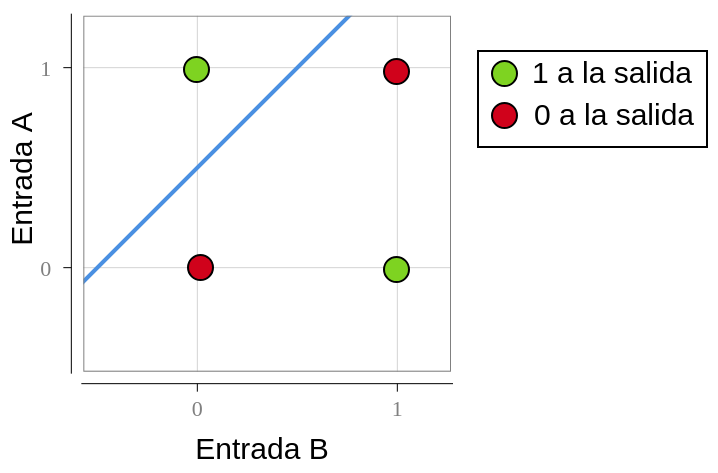
\includegraphics[width=\textwidth]{imagenes/diagramaXor.png}
	\end{minipage}
	\caption{No es posible separar con una capa de perceptrón la salida de una compuerta XOR. (Imagen de autoría propia)}
	\label{fig:xor}
\end{figure}
		       
		       
\par Como se ve en la figura \ref{fig:xor} para poder resolver este tipo de problemas se propuso usar mas capas del perceptrón que podrían resolver el problema fácilmente. Ya que cuando se agregan más perceptrones se pueden \textit{`dibujar'} más lineas que puedan ayudarnos a dividir mejor una clase.
		    
\begin{figure}[H]
	\centering
	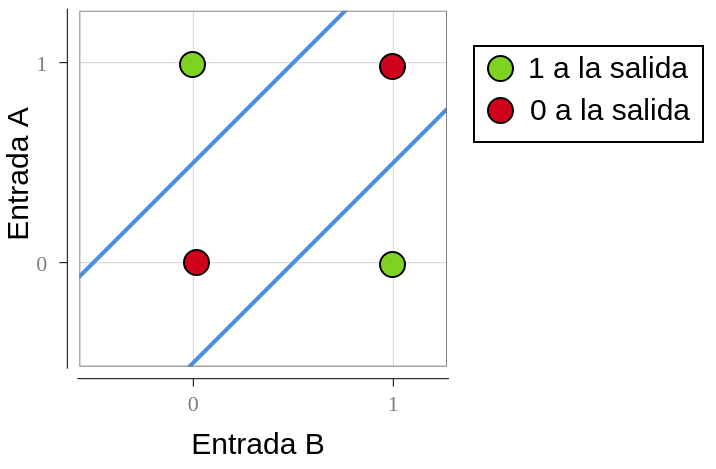
\includegraphics[width=0.5\textwidth]{imagenes/diagramaXor2.png}
	\caption{Usando una capa más se puede dividir la salida de la compuerta XOR. (Imagen de autoría propia)}
	\label{fig:xor2}
\end{figure}
		    
\par Al concepto de red neuronal, como un conjunto de perceptrones interconectados que hacen aún más compleja la salida de un simple perceptrón, se le conoce varios nombres como son \textit{fully connected}, \textit{\gls{mlp}} y red neuronal completamente conectada. Para el caso de cada perceptrón deberán aplicarse las mismas operaciones que se habían descrito para un solo perceptrón, en la figura \ref{fig:redneuronal1} se puede observar como se calcula la salida de la primera neurona de la primera capa.
		    
\begin{figure}[H]
	\centering
	

\tikzset{every picture/.style={line width=0.75pt}} %set default line width to 0.75pt        

\begin{tikzpicture}[x=0.75pt,y=0.75pt,yscale=-1,xscale=1]
%uncomment if require: \path (0,320); %set diagram left start at 0, and has height of 320

%Straight Lines [id:da8798173448108342] 
\draw [color={rgb, 255:red, 155; green, 155; blue, 155 }  ,draw opacity=1 ]   (93.5,67.25) -- (130.19,150.42) ;
\draw [shift={(131,152.25)}, rotate = 246.19] [fill={rgb, 255:red, 155; green, 155; blue, 155 }  ,fill opacity=1 ][line width=0.75]  [draw opacity=0] (8.93,-4.29) -- (0,0) -- (8.93,4.29) -- cycle    ;

%Straight Lines [id:da1264938029525713] 
\draw [color={rgb, 255:red, 155; green, 155; blue, 155 }  ,draw opacity=1 ]   (93.5,67.25) -- (132.57,243.3) ;
\draw [shift={(133,245.25)}, rotate = 257.49] [fill={rgb, 255:red, 155; green, 155; blue, 155 }  ,fill opacity=1 ][line width=0.75]  [draw opacity=0] (8.93,-4.29) -- (0,0) -- (8.93,4.29) -- cycle    ;

%Straight Lines [id:da4251940989802534] 
\draw [color={rgb, 255:red, 155; green, 155; blue, 155 }  ,draw opacity=1 ]   (93.5,116.25) -- (129.56,150.86) ;
\draw [shift={(131,152.25)}, rotate = 223.82999999999998] [fill={rgb, 255:red, 155; green, 155; blue, 155 }  ,fill opacity=1 ][line width=0.75]  [draw opacity=0] (8.93,-4.29) -- (0,0) -- (8.93,4.29) -- cycle    ;

%Straight Lines [id:da608901596398933] 
\draw [color={rgb, 255:red, 155; green, 155; blue, 155 }  ,draw opacity=1 ]   (93.5,116.25) -- (132.41,243.34) ;
\draw [shift={(133,245.25)}, rotate = 252.98000000000002] [fill={rgb, 255:red, 155; green, 155; blue, 155 }  ,fill opacity=1 ][line width=0.75]  [draw opacity=0] (8.93,-4.29) -- (0,0) -- (8.93,4.29) -- cycle    ;

%Straight Lines [id:da22280654479157525] 
\draw [color={rgb, 255:red, 155; green, 155; blue, 155 }  ,draw opacity=1 ]   (94.5,163.25) -- (129.09,152.83) ;
\draw [shift={(131,152.25)}, rotate = 523.23] [fill={rgb, 255:red, 155; green, 155; blue, 155 }  ,fill opacity=1 ][line width=0.75]  [draw opacity=0] (8.93,-4.29) -- (0,0) -- (8.93,4.29) -- cycle    ;

%Straight Lines [id:da6030354960312154] 
\draw [color={rgb, 255:red, 155; green, 155; blue, 155 }  ,draw opacity=1 ]   (94.5,163.25) -- (132.15,243.44) ;
\draw [shift={(133,245.25)}, rotate = 244.85] [fill={rgb, 255:red, 155; green, 155; blue, 155 }  ,fill opacity=1 ][line width=0.75]  [draw opacity=0] (8.93,-4.29) -- (0,0) -- (8.93,4.29) -- cycle    ;

%Straight Lines [id:da21636688103646295] 
\draw [color={rgb, 255:red, 155; green, 155; blue, 155 }  ,draw opacity=1 ]   (95.5,236.25) -- (130.22,154.09) ;
\draw [shift={(131,152.25)}, rotate = 472.91] [fill={rgb, 255:red, 155; green, 155; blue, 155 }  ,fill opacity=1 ][line width=0.75]  [draw opacity=0] (8.93,-4.29) -- (0,0) -- (8.93,4.29) -- cycle    ;

%Straight Lines [id:da5980881110108045] 
\draw [color={rgb, 255:red, 155; green, 155; blue, 155 }  ,draw opacity=1 ]   (95.5,236.25) -- (131.06,244.78) ;
\draw [shift={(133,245.25)}, rotate = 193.5] [fill={rgb, 255:red, 155; green, 155; blue, 155 }  ,fill opacity=1 ][line width=0.75]  [draw opacity=0] (8.93,-4.29) -- (0,0) -- (8.93,4.29) -- cycle    ;

%Straight Lines [id:da3351006204177107] 
\draw [color={rgb, 255:red, 155; green, 155; blue, 155 }  ,draw opacity=1 ]   (248.5,42.25) -- (285.24,62.29) ;
\draw [shift={(287,63.25)}, rotate = 208.61] [fill={rgb, 255:red, 155; green, 155; blue, 155 }  ,fill opacity=1 ][line width=0.75]  [draw opacity=0] (8.93,-4.29) -- (0,0) -- (8.93,4.29) -- cycle    ;

%Straight Lines [id:da6626680795590805] 
\draw [color={rgb, 255:red, 155; green, 155; blue, 155 }  ,draw opacity=1 ]   (248.5,42.25) -- (285.07,111.48) ;
\draw [shift={(286,113.25)}, rotate = 242.16] [fill={rgb, 255:red, 155; green, 155; blue, 155 }  ,fill opacity=1 ][line width=0.75]  [draw opacity=0] (8.93,-4.29) -- (0,0) -- (8.93,4.29) -- cycle    ;

%Straight Lines [id:da7726736210859901] 
\draw [color={rgb, 255:red, 155; green, 155; blue, 155 }  ,draw opacity=1 ]   (248.5,42.25) -- (286.38,158.35) ;
\draw [shift={(287,160.25)}, rotate = 251.93] [fill={rgb, 255:red, 155; green, 155; blue, 155 }  ,fill opacity=1 ][line width=0.75]  [draw opacity=0] (8.93,-4.29) -- (0,0) -- (8.93,4.29) -- cycle    ;

%Straight Lines [id:da6779074339555233] 
\draw [color={rgb, 255:red, 155; green, 155; blue, 155 }  ,draw opacity=1 ]   (248.5,42.25) -- (287.59,231.29) ;
\draw [shift={(288,233.25)}, rotate = 258.32] [fill={rgb, 255:red, 155; green, 155; blue, 155 }  ,fill opacity=1 ][line width=0.75]  [draw opacity=0] (8.93,-4.29) -- (0,0) -- (8.93,4.29) -- cycle    ;

%Straight Lines [id:da22497111902415767] 
\draw [color={rgb, 255:red, 155; green, 155; blue, 155 }  ,draw opacity=1 ]   (247.5,97.25) -- (285.48,64.55) ;
\draw [shift={(287,63.25)}, rotate = 499.28] [fill={rgb, 255:red, 155; green, 155; blue, 155 }  ,fill opacity=1 ][line width=0.75]  [draw opacity=0] (8.93,-4.29) -- (0,0) -- (8.93,4.29) -- cycle    ;

%Straight Lines [id:da7915744230148478] 
\draw [color={rgb, 255:red, 155; green, 155; blue, 155 }  ,draw opacity=1 ]   (247.5,97.25) -- (284.15,112.48) ;
\draw [shift={(286,113.25)}, rotate = 202.57] [fill={rgb, 255:red, 155; green, 155; blue, 155 }  ,fill opacity=1 ][line width=0.75]  [draw opacity=0] (8.93,-4.29) -- (0,0) -- (8.93,4.29) -- cycle    ;

%Straight Lines [id:da8444489661109031] 
\draw [color={rgb, 255:red, 155; green, 155; blue, 155 }  ,draw opacity=1 ]   (247.5,97.25) -- (287.43,231.33) ;
\draw [shift={(288,233.25)}, rotate = 253.42000000000002] [fill={rgb, 255:red, 155; green, 155; blue, 155 }  ,fill opacity=1 ][line width=0.75]  [draw opacity=0] (8.93,-4.29) -- (0,0) -- (8.93,4.29) -- cycle    ;

%Straight Lines [id:da180467501143327] 
\draw [color={rgb, 255:red, 155; green, 155; blue, 155 }  ,draw opacity=1 ]   (247.5,152.25) -- (286.19,65.08) ;
\draw [shift={(287,63.25)}, rotate = 473.93] [fill={rgb, 255:red, 155; green, 155; blue, 155 }  ,fill opacity=1 ][line width=0.75]  [draw opacity=0] (8.93,-4.29) -- (0,0) -- (8.93,4.29) -- cycle    ;

%Straight Lines [id:da7179418865674392] 
\draw [color={rgb, 255:red, 155; green, 155; blue, 155 }  ,draw opacity=1 ]   (247.5,152.25) -- (284.59,114.67) ;
\draw [shift={(286,113.25)}, rotate = 494.63] [fill={rgb, 255:red, 155; green, 155; blue, 155 }  ,fill opacity=1 ][line width=0.75]  [draw opacity=0] (8.93,-4.29) -- (0,0) -- (8.93,4.29) -- cycle    ;

%Straight Lines [id:da35423297686642163] 
\draw [color={rgb, 255:red, 155; green, 155; blue, 155 }  ,draw opacity=1 ]   (247.5,152.25) -- (285.04,159.85) ;
\draw [shift={(287,160.25)}, rotate = 191.45] [fill={rgb, 255:red, 155; green, 155; blue, 155 }  ,fill opacity=1 ][line width=0.75]  [draw opacity=0] (8.93,-4.29) -- (0,0) -- (8.93,4.29) -- cycle    ;

%Straight Lines [id:da8222185311967365] 
\draw [color={rgb, 255:red, 155; green, 155; blue, 155 }  ,draw opacity=1 ]   (247.5,152.25) -- (287.11,231.46) ;
\draw [shift={(288,233.25)}, rotate = 243.43] [fill={rgb, 255:red, 155; green, 155; blue, 155 }  ,fill opacity=1 ][line width=0.75]  [draw opacity=0] (8.93,-4.29) -- (0,0) -- (8.93,4.29) -- cycle    ;

%Straight Lines [id:da6366233578085132] 
\draw [color={rgb, 255:red, 155; green, 155; blue, 155 }  ,draw opacity=1 ]   (249.5,245.25) -- (286.6,65.21) ;
\draw [shift={(287,63.25)}, rotate = 461.64] [fill={rgb, 255:red, 155; green, 155; blue, 155 }  ,fill opacity=1 ][line width=0.75]  [draw opacity=0] (8.93,-4.29) -- (0,0) -- (8.93,4.29) -- cycle    ;

%Straight Lines [id:da19092990208654426] 
\draw [color={rgb, 255:red, 155; green, 155; blue, 155 }  ,draw opacity=1 ]   (249.5,245.25) -- (285.47,115.18) ;
\draw [shift={(286,113.25)}, rotate = 465.46] [fill={rgb, 255:red, 155; green, 155; blue, 155 }  ,fill opacity=1 ][line width=0.75]  [draw opacity=0] (8.93,-4.29) -- (0,0) -- (8.93,4.29) -- cycle    ;

%Straight Lines [id:da5250825232708285] 
\draw [color={rgb, 255:red, 155; green, 155; blue, 155 }  ,draw opacity=1 ]   (249.5,245.25) -- (286.19,162.08) ;
\draw [shift={(287,160.25)}, rotate = 473.81] [fill={rgb, 255:red, 155; green, 155; blue, 155 }  ,fill opacity=1 ][line width=0.75]  [draw opacity=0] (8.93,-4.29) -- (0,0) -- (8.93,4.29) -- cycle    ;

%Straight Lines [id:da06185650174435953] 
\draw [color={rgb, 255:red, 155; green, 155; blue, 155 }  ,draw opacity=1 ]   (249.5,245.25) -- (286.09,233.85) ;
\draw [shift={(288,233.25)}, rotate = 522.69] [fill={rgb, 255:red, 155; green, 155; blue, 155 }  ,fill opacity=1 ][line width=0.75]  [draw opacity=0] (8.93,-4.29) -- (0,0) -- (8.93,4.29) -- cycle    ;

%Shape: Circle [id:dp8378261731976331] 
\draw   (60,66.25) .. controls (60,56.72) and (67.72,49) .. (77.25,49) .. controls (86.78,49) and (94.5,56.72) .. (94.5,66.25) .. controls (94.5,75.78) and (86.78,83.5) .. (77.25,83.5) .. controls (67.72,83.5) and (60,75.78) .. (60,66.25) -- cycle ;
%Shape: Circle [id:dp6886548408081758] 
\draw   (61,236.25) .. controls (61,226.72) and (68.72,219) .. (78.25,219) .. controls (87.78,219) and (95.5,226.72) .. (95.5,236.25) .. controls (95.5,245.78) and (87.78,253.5) .. (78.25,253.5) .. controls (68.72,253.5) and (61,245.78) .. (61,236.25) -- cycle ;
%Shape: Circle [id:dp46631909550454664] 
\draw   (59,116.25) .. controls (59,106.72) and (66.72,99) .. (76.25,99) .. controls (85.78,99) and (93.5,106.72) .. (93.5,116.25) .. controls (93.5,125.78) and (85.78,133.5) .. (76.25,133.5) .. controls (66.72,133.5) and (59,125.78) .. (59,116.25) -- cycle ;
%Shape: Circle [id:dp624774125190017] 
\draw   (60,163.25) .. controls (60,153.72) and (67.72,146) .. (77.25,146) .. controls (86.78,146) and (94.5,153.72) .. (94.5,163.25) .. controls (94.5,172.78) and (86.78,180.5) .. (77.25,180.5) .. controls (67.72,180.5) and (60,172.78) .. (60,163.25) -- cycle ;
%Straight Lines [id:da4326296089497377] 
\draw    (41.02,66.25) -- (58,66.25) ;
\draw [shift={(60,66.25)}, rotate = 180] [fill={rgb, 255:red, 0; green, 0; blue, 0 }  ][line width=0.75]  [draw opacity=0] (8.93,-4.29) -- (0,0) -- (8.93,4.29) -- cycle    ;

%Straight Lines [id:da7377396516203609] 
\draw    (40.02,116.25) -- (57,116.25) ;
\draw [shift={(59,116.25)}, rotate = 180] [fill={rgb, 255:red, 0; green, 0; blue, 0 }  ][line width=0.75]  [draw opacity=0] (8.93,-4.29) -- (0,0) -- (8.93,4.29) -- cycle    ;

%Straight Lines [id:da772460813491475] 
\draw    (41.02,163.25) -- (58,163.25) ;
\draw [shift={(60,163.25)}, rotate = 180] [fill={rgb, 255:red, 0; green, 0; blue, 0 }  ][line width=0.75]  [draw opacity=0] (8.93,-4.29) -- (0,0) -- (8.93,4.29) -- cycle    ;

%Straight Lines [id:da9681905997792641] 
\draw    (42.02,236.25) -- (59,236.25) ;
\draw [shift={(61,236.25)}, rotate = 180] [fill={rgb, 255:red, 0; green, 0; blue, 0 }  ][line width=0.75]  [draw opacity=0] (8.93,-4.29) -- (0,0) -- (8.93,4.29) -- cycle    ;

%Shape: Circle [id:dp21825918883593576] 
\draw   (132,42.25) .. controls (132,32.72) and (139.72,25) .. (149.25,25) .. controls (158.78,25) and (166.5,32.72) .. (166.5,42.25) .. controls (166.5,51.78) and (158.78,59.5) .. (149.25,59.5) .. controls (139.72,59.5) and (132,51.78) .. (132,42.25) -- cycle ;
%Shape: Circle [id:dp547845684421643] 
\draw   (133,245.25) .. controls (133,235.72) and (140.72,228) .. (150.25,228) .. controls (159.78,228) and (167.5,235.72) .. (167.5,245.25) .. controls (167.5,254.78) and (159.78,262.5) .. (150.25,262.5) .. controls (140.72,262.5) and (133,254.78) .. (133,245.25) -- cycle ;
%Shape: Circle [id:dp8711680643696975] 
\draw   (131,97.25) .. controls (131,87.72) and (138.72,80) .. (148.25,80) .. controls (157.78,80) and (165.5,87.72) .. (165.5,97.25) .. controls (165.5,106.78) and (157.78,114.5) .. (148.25,114.5) .. controls (138.72,114.5) and (131,106.78) .. (131,97.25) -- cycle ;
%Shape: Circle [id:dp8241885312698898] 
\draw   (131,152.25) .. controls (131,142.72) and (138.72,135) .. (148.25,135) .. controls (157.78,135) and (165.5,142.72) .. (165.5,152.25) .. controls (165.5,161.78) and (157.78,169.5) .. (148.25,169.5) .. controls (138.72,169.5) and (131,161.78) .. (131,152.25) -- cycle ;
%Shape: Circle [id:dp7119276185561412] 
\draw   (214,42.25) .. controls (214,32.72) and (221.72,25) .. (231.25,25) .. controls (240.78,25) and (248.5,32.72) .. (248.5,42.25) .. controls (248.5,51.78) and (240.78,59.5) .. (231.25,59.5) .. controls (221.72,59.5) and (214,51.78) .. (214,42.25) -- cycle ;
%Shape: Circle [id:dp3179021384105416] 
\draw   (215,245.25) .. controls (215,235.72) and (222.72,228) .. (232.25,228) .. controls (241.78,228) and (249.5,235.72) .. (249.5,245.25) .. controls (249.5,254.78) and (241.78,262.5) .. (232.25,262.5) .. controls (222.72,262.5) and (215,254.78) .. (215,245.25) -- cycle ;
%Shape: Circle [id:dp8755056890726975] 
\draw   (213,97.25) .. controls (213,87.72) and (220.72,80) .. (230.25,80) .. controls (239.78,80) and (247.5,87.72) .. (247.5,97.25) .. controls (247.5,106.78) and (239.78,114.5) .. (230.25,114.5) .. controls (220.72,114.5) and (213,106.78) .. (213,97.25) -- cycle ;
%Shape: Circle [id:dp4747564535552429] 
\draw   (213,152.25) .. controls (213,142.72) and (220.72,135) .. (230.25,135) .. controls (239.78,135) and (247.5,142.72) .. (247.5,152.25) .. controls (247.5,161.78) and (239.78,169.5) .. (230.25,169.5) .. controls (220.72,169.5) and (213,161.78) .. (213,152.25) -- cycle ;
%Shape: Circle [id:dp8197699354277264] 
\draw   (287,63.25) .. controls (287,53.72) and (294.72,46) .. (304.25,46) .. controls (313.78,46) and (321.5,53.72) .. (321.5,63.25) .. controls (321.5,72.78) and (313.78,80.5) .. (304.25,80.5) .. controls (294.72,80.5) and (287,72.78) .. (287,63.25) -- cycle ;
%Shape: Circle [id:dp8721964334353247] 
\draw   (288,233.25) .. controls (288,223.72) and (295.72,216) .. (305.25,216) .. controls (314.78,216) and (322.5,223.72) .. (322.5,233.25) .. controls (322.5,242.78) and (314.78,250.5) .. (305.25,250.5) .. controls (295.72,250.5) and (288,242.78) .. (288,233.25) -- cycle ;
%Shape: Circle [id:dp5987591258534826] 
\draw   (286,113.25) .. controls (286,103.72) and (293.72,96) .. (303.25,96) .. controls (312.78,96) and (320.5,103.72) .. (320.5,113.25) .. controls (320.5,122.78) and (312.78,130.5) .. (303.25,130.5) .. controls (293.72,130.5) and (286,122.78) .. (286,113.25) -- cycle ;
%Shape: Circle [id:dp49752905656026436] 
\draw   (287,160.25) .. controls (287,150.72) and (294.72,143) .. (304.25,143) .. controls (313.78,143) and (321.5,150.72) .. (321.5,160.25) .. controls (321.5,169.78) and (313.78,177.5) .. (304.25,177.5) .. controls (294.72,177.5) and (287,169.78) .. (287,160.25) -- cycle ;
%Straight Lines [id:da2893286552413561] 
\draw    (322.02,63.25) -- (339,63.25) ;
\draw [shift={(341,63.25)}, rotate = 180] [fill={rgb, 255:red, 0; green, 0; blue, 0 }  ][line width=0.75]  [draw opacity=0] (8.93,-4.29) -- (0,0) -- (8.93,4.29) -- cycle    ;

%Straight Lines [id:da31837181970999007] 
\draw    (321.02,113.25) -- (338,113.25) ;
\draw [shift={(340,113.25)}, rotate = 180] [fill={rgb, 255:red, 0; green, 0; blue, 0 }  ][line width=0.75]  [draw opacity=0] (8.93,-4.29) -- (0,0) -- (8.93,4.29) -- cycle    ;

%Straight Lines [id:da7130677314020706] 
\draw    (322.02,160.25) -- (339,160.25) ;
\draw [shift={(341,160.25)}, rotate = 180] [fill={rgb, 255:red, 0; green, 0; blue, 0 }  ][line width=0.75]  [draw opacity=0] (8.93,-4.29) -- (0,0) -- (8.93,4.29) -- cycle    ;

%Straight Lines [id:da1146408293027561] 
\draw    (323.02,233.25) -- (340,233.25) ;
\draw [shift={(342,233.25)}, rotate = 180] [fill={rgb, 255:red, 0; green, 0; blue, 0 }  ][line width=0.75]  [draw opacity=0] (8.93,-4.29) -- (0,0) -- (8.93,4.29) -- cycle    ;

%Straight Lines [id:da9370970117900812] 
\draw [color={rgb, 255:red, 208; green, 2; blue, 27 }  ,draw opacity=1 ]   (94.5,66.25) -- (129.48,95.96) ;
\draw [shift={(131,97.25)}, rotate = 220.34] [fill={rgb, 255:red, 208; green, 2; blue, 27 }  ,fill opacity=1 ][line width=0.75]  [draw opacity=0] (8.93,-4.29) -- (0,0) -- (8.93,4.29) -- cycle    ;

%Straight Lines [id:da31070588195621585] 
\draw [color={rgb, 255:red, 208; green, 2; blue, 27 }  ,draw opacity=1 ]   (93.5,116.25) -- (129.22,98.15) ;
\draw [shift={(131,97.25)}, rotate = 513.13] [fill={rgb, 255:red, 208; green, 2; blue, 27 }  ,fill opacity=1 ][line width=0.75]  [draw opacity=0] (8.93,-4.29) -- (0,0) -- (8.93,4.29) -- cycle    ;

%Straight Lines [id:da8021804321980563] 
\draw [color={rgb, 255:red, 208; green, 2; blue, 27 }  ,draw opacity=1 ]   (94.5,163.25) -- (130.03,99) ;
\draw [shift={(131,97.25)}, rotate = 478.94] [fill={rgb, 255:red, 208; green, 2; blue, 27 }  ,fill opacity=1 ][line width=0.75]  [draw opacity=0] (8.93,-4.29) -- (0,0) -- (8.93,4.29) -- cycle    ;

%Straight Lines [id:da2185947312717822] 
\draw [color={rgb, 255:red, 208; green, 2; blue, 27 }  ,draw opacity=1 ]   (95.5,236.25) -- (130.51,99.19) ;
\draw [shift={(131,97.25)}, rotate = 464.33] [fill={rgb, 255:red, 208; green, 2; blue, 27 }  ,fill opacity=1 ][line width=0.75]  [draw opacity=0] (8.93,-4.29) -- (0,0) -- (8.93,4.29) -- cycle    ;



% Text Node
\draw (80,201) node [rotate=-90] [align=left] {\textbf{{\large . . .}}};
% Text Node
\draw (152,196) node [rotate=-90] [align=left] {\textbf{{\large . . .}}};
% Text Node
\draw (192,132) node  [align=left] {\textbf{{\large . . .}}};
% Text Node
\draw (234,196) node [rotate=-90] [align=left] {\textbf{{\large . . .}}};
% Text Node
\draw (307,198) node [rotate=-90] [align=left] {\textbf{{\large . . .}}};
% Text Node
\draw (78,66) node   {$1$};
% Text Node
\draw (78,118) node   {$x_{1}$};
% Text Node
\draw (78,163) node   {$x_{2}$};
% Text Node
\draw (79,236) node   {$x_{n}$};
% Text Node
\draw (150,44) node   {$1$};
% Text Node
\draw (149,97) node   {$a^{1}_{1}$};
% Text Node
\draw (149,153) node   {$a^{1}_{2}$};
% Text Node
\draw (151,246) node   {$a^{1}_{m}$};
% Text Node
\draw (232,43) node   {$1$};
% Text Node
\draw (231,97) node   {$a^{k}_{1}$};
% Text Node
\draw (230,151) node   {$a^{k}_{2}$};
% Text Node
\draw (234,244) node   {$a^{k}_{m}$};
% Text Node
\draw (305,63) node   {$y_{1}$};
% Text Node
\draw (304,112) node   {$y_{2}$};
% Text Node
\draw (304,161) node   {$y_{3}$};
% Text Node
\draw (306,232) node   {$y_{l}$};
% Text Node
\draw (111,58) node   {$\theta ^{1}_{01}$};
% Text Node
\draw (105,94) node   {$\theta ^{1}_{11}$};
% Text Node
\draw (102,133) node   {$\theta ^{1}_{21}$};
% Text Node
\draw (117,209) node   {$\theta ^{1}_{n1}$};
% Text Node
\draw (240,283) node   {${\textstyle a^{1}_{1} =f\left( 1\times \theta ^{1}_{01} +x_{1} \times \theta ^{1}_{11} +x_{2} \times \theta ^{1}_{21} +.\ .\ .+x_{n} \times \theta ^{1}_{n1}\right) =f\left( x^{T} \Theta ^{1}_{1}\right)}$};
% Text Node
\draw (445,98) node   {$x=\begin{bmatrix}
1\\
x_{1}\\
x_{2}\\
...\\
x_{n}
\end{bmatrix} \ ;\ \Theta ^{i}_{j} =\begin{bmatrix}
\theta ^{i}_{0}\\
\theta ^{i}_{1}\\
\theta ^{i}_{2}\\
...\\
\theta ^{i}_{n}
\end{bmatrix}$};


\end{tikzpicture}

	\caption{Cálculo de la salida de la primera neurona de la primera capa de una red neuronal \gls{mlp} (Imagen de autoría propia).}
	\label{fig:redneuronal1}
\end{figure}
		    
		    
\begin{figure}
	\centering
	

\tikzset{every picture/.style={line width=0.75pt}} %set default line width to 0.75pt        

\begin{tikzpicture}[x=0.75pt,y=0.75pt,yscale=-1,xscale=1]
%uncomment if require: \path (0,300); %set diagram left start at 0, and has height of 300

%Shape: Circle [id:dp5524582775574844] 
\draw   (88,72.25) .. controls (88,62.72) and (95.72,55) .. (105.25,55) .. controls (114.78,55) and (122.5,62.72) .. (122.5,72.25) .. controls (122.5,81.78) and (114.78,89.5) .. (105.25,89.5) .. controls (95.72,89.5) and (88,81.78) .. (88,72.25) -- cycle ;
%Shape: Circle [id:dp9055284592778006] 
\draw   (89,242.25) .. controls (89,232.72) and (96.72,225) .. (106.25,225) .. controls (115.78,225) and (123.5,232.72) .. (123.5,242.25) .. controls (123.5,251.78) and (115.78,259.5) .. (106.25,259.5) .. controls (96.72,259.5) and (89,251.78) .. (89,242.25) -- cycle ;
%Shape: Circle [id:dp1656948629963515] 
\draw   (87,122.25) .. controls (87,112.72) and (94.72,105) .. (104.25,105) .. controls (113.78,105) and (121.5,112.72) .. (121.5,122.25) .. controls (121.5,131.78) and (113.78,139.5) .. (104.25,139.5) .. controls (94.72,139.5) and (87,131.78) .. (87,122.25) -- cycle ;
%Shape: Circle [id:dp606031338973398] 
\draw   (88,169.25) .. controls (88,159.72) and (95.72,152) .. (105.25,152) .. controls (114.78,152) and (122.5,159.72) .. (122.5,169.25) .. controls (122.5,178.78) and (114.78,186.5) .. (105.25,186.5) .. controls (95.72,186.5) and (88,178.78) .. (88,169.25) -- cycle ;
%Straight Lines [id:da7583336175527668] 
\draw    (69.02,72.25) -- (86,72.25) ;
\draw [shift={(88,72.25)}, rotate = 180] [fill={rgb, 255:red, 0; green, 0; blue, 0 }  ][line width=0.75]  [draw opacity=0] (8.93,-4.29) -- (0,0) -- (8.93,4.29) -- cycle    ;

%Straight Lines [id:da33136749911196883] 
\draw    (68.02,122.25) -- (85,122.25) ;
\draw [shift={(87,122.25)}, rotate = 180] [fill={rgb, 255:red, 0; green, 0; blue, 0 }  ][line width=0.75]  [draw opacity=0] (8.93,-4.29) -- (0,0) -- (8.93,4.29) -- cycle    ;

%Straight Lines [id:da4263129214891306] 
\draw    (69.02,169.25) -- (86,169.25) ;
\draw [shift={(88,169.25)}, rotate = 180] [fill={rgb, 255:red, 0; green, 0; blue, 0 }  ][line width=0.75]  [draw opacity=0] (8.93,-4.29) -- (0,0) -- (8.93,4.29) -- cycle    ;

%Straight Lines [id:da05901696855647298] 
\draw    (70.02,242.25) -- (87,242.25) ;
\draw [shift={(89,242.25)}, rotate = 180] [fill={rgb, 255:red, 0; green, 0; blue, 0 }  ][line width=0.75]  [draw opacity=0] (8.93,-4.29) -- (0,0) -- (8.93,4.29) -- cycle    ;

%Shape: Circle [id:dp7811394509655811] 
\draw   (160,48.25) .. controls (160,38.72) and (167.72,31) .. (177.25,31) .. controls (186.78,31) and (194.5,38.72) .. (194.5,48.25) .. controls (194.5,57.78) and (186.78,65.5) .. (177.25,65.5) .. controls (167.72,65.5) and (160,57.78) .. (160,48.25) -- cycle ;
%Shape: Circle [id:dp9905693780000109] 
\draw   (161,251.25) .. controls (161,241.72) and (168.72,234) .. (178.25,234) .. controls (187.78,234) and (195.5,241.72) .. (195.5,251.25) .. controls (195.5,260.78) and (187.78,268.5) .. (178.25,268.5) .. controls (168.72,268.5) and (161,260.78) .. (161,251.25) -- cycle ;
%Shape: Circle [id:dp10282768320714131] 
\draw  [color={rgb, 255:red, 155; green, 155; blue, 155 }  ,draw opacity=1 ] (159,103.25) .. controls (159,93.72) and (166.72,86) .. (176.25,86) .. controls (185.78,86) and (193.5,93.72) .. (193.5,103.25) .. controls (193.5,112.78) and (185.78,120.5) .. (176.25,120.5) .. controls (166.72,120.5) and (159,112.78) .. (159,103.25) -- cycle ;
%Shape: Circle [id:dp8751704729152276] 
\draw   (159,158.25) .. controls (159,148.72) and (166.72,141) .. (176.25,141) .. controls (185.78,141) and (193.5,148.72) .. (193.5,158.25) .. controls (193.5,167.78) and (185.78,175.5) .. (176.25,175.5) .. controls (166.72,175.5) and (159,167.78) .. (159,158.25) -- cycle ;
%Shape: Circle [id:dp14191125242712754] 
\draw   (242,48.25) .. controls (242,38.72) and (249.72,31) .. (259.25,31) .. controls (268.78,31) and (276.5,38.72) .. (276.5,48.25) .. controls (276.5,57.78) and (268.78,65.5) .. (259.25,65.5) .. controls (249.72,65.5) and (242,57.78) .. (242,48.25) -- cycle ;
%Shape: Circle [id:dp5157180132102686] 
\draw   (243,251.25) .. controls (243,241.72) and (250.72,234) .. (260.25,234) .. controls (269.78,234) and (277.5,241.72) .. (277.5,251.25) .. controls (277.5,260.78) and (269.78,268.5) .. (260.25,268.5) .. controls (250.72,268.5) and (243,260.78) .. (243,251.25) -- cycle ;
%Shape: Circle [id:dp8690128913833901] 
\draw   (241,103.25) .. controls (241,93.72) and (248.72,86) .. (258.25,86) .. controls (267.78,86) and (275.5,93.72) .. (275.5,103.25) .. controls (275.5,112.78) and (267.78,120.5) .. (258.25,120.5) .. controls (248.72,120.5) and (241,112.78) .. (241,103.25) -- cycle ;
%Shape: Circle [id:dp9649278733196962] 
\draw   (241,158.25) .. controls (241,148.72) and (248.72,141) .. (258.25,141) .. controls (267.78,141) and (275.5,148.72) .. (275.5,158.25) .. controls (275.5,167.78) and (267.78,175.5) .. (258.25,175.5) .. controls (248.72,175.5) and (241,167.78) .. (241,158.25) -- cycle ;
%Shape: Circle [id:dp1953350433383112] 
\draw   (315,69.25) .. controls (315,59.72) and (322.72,52) .. (332.25,52) .. controls (341.78,52) and (349.5,59.72) .. (349.5,69.25) .. controls (349.5,78.78) and (341.78,86.5) .. (332.25,86.5) .. controls (322.72,86.5) and (315,78.78) .. (315,69.25) -- cycle ;
%Shape: Circle [id:dp31843323470147866] 
\draw   (316,239.25) .. controls (316,229.72) and (323.72,222) .. (333.25,222) .. controls (342.78,222) and (350.5,229.72) .. (350.5,239.25) .. controls (350.5,248.78) and (342.78,256.5) .. (333.25,256.5) .. controls (323.72,256.5) and (316,248.78) .. (316,239.25) -- cycle ;
%Shape: Circle [id:dp7000306624407344] 
\draw   (314,119.25) .. controls (314,109.72) and (321.72,102) .. (331.25,102) .. controls (340.78,102) and (348.5,109.72) .. (348.5,119.25) .. controls (348.5,128.78) and (340.78,136.5) .. (331.25,136.5) .. controls (321.72,136.5) and (314,128.78) .. (314,119.25) -- cycle ;
%Shape: Circle [id:dp10864162142112854] 
\draw   (315,166.25) .. controls (315,156.72) and (322.72,149) .. (332.25,149) .. controls (341.78,149) and (349.5,156.72) .. (349.5,166.25) .. controls (349.5,175.78) and (341.78,183.5) .. (332.25,183.5) .. controls (322.72,183.5) and (315,175.78) .. (315,166.25) -- cycle ;
%Straight Lines [id:da9597423511061334] 
\draw    (350.02,69.25) -- (367,69.25) ;
\draw [shift={(369,69.25)}, rotate = 180] [fill={rgb, 255:red, 0; green, 0; blue, 0 }  ][line width=0.75]  [draw opacity=0] (8.93,-4.29) -- (0,0) -- (8.93,4.29) -- cycle    ;

%Straight Lines [id:da05206380931890586] 
\draw    (349.02,119.25) -- (366,119.25) ;
\draw [shift={(368,119.25)}, rotate = 180] [fill={rgb, 255:red, 0; green, 0; blue, 0 }  ][line width=0.75]  [draw opacity=0] (8.93,-4.29) -- (0,0) -- (8.93,4.29) -- cycle    ;

%Straight Lines [id:da5095484827545105] 
\draw    (350.02,166.25) -- (367,166.25) ;
\draw [shift={(369,166.25)}, rotate = 180] [fill={rgb, 255:red, 0; green, 0; blue, 0 }  ][line width=0.75]  [draw opacity=0] (8.93,-4.29) -- (0,0) -- (8.93,4.29) -- cycle    ;

%Straight Lines [id:da6172822793664112] 
\draw    (351.02,239.25) -- (368,239.25) ;
\draw [shift={(370,239.25)}, rotate = 180] [fill={rgb, 255:red, 0; green, 0; blue, 0 }  ][line width=0.75]  [draw opacity=0] (8.93,-4.29) -- (0,0) -- (8.93,4.29) -- cycle    ;

%Straight Lines [id:da8294435479357769] 
\draw [color={rgb, 255:red, 155; green, 155; blue, 155 }  ,draw opacity=1 ]   (122.5,72.25) -- (157.48,101.96) ;
\draw [shift={(159,103.25)}, rotate = 220.34] [fill={rgb, 255:red, 155; green, 155; blue, 155 }  ,fill opacity=1 ][line width=0.75]  [draw opacity=0] (8.93,-4.29) -- (0,0) -- (8.93,4.29) -- cycle    ;

%Straight Lines [id:da6143981027876961] 
\draw [color={rgb, 255:red, 155; green, 155; blue, 155 }  ,draw opacity=1 ]   (121.5,122.25) -- (157.22,104.15) ;
\draw [shift={(159,103.25)}, rotate = 513.13] [fill={rgb, 255:red, 155; green, 155; blue, 155 }  ,fill opacity=1 ][line width=0.75]  [draw opacity=0] (8.93,-4.29) -- (0,0) -- (8.93,4.29) -- cycle    ;

%Straight Lines [id:da8989735465663513] 
\draw [color={rgb, 255:red, 155; green, 155; blue, 155 }  ,draw opacity=1 ]   (122.5,169.25) -- (158.03,105) ;
\draw [shift={(159,103.25)}, rotate = 478.94] [fill={rgb, 255:red, 155; green, 155; blue, 155 }  ,fill opacity=1 ][line width=0.75]  [draw opacity=0] (8.93,-4.29) -- (0,0) -- (8.93,4.29) -- cycle    ;

%Straight Lines [id:da18190387914988415] 
\draw [color={rgb, 255:red, 155; green, 155; blue, 155 }  ,draw opacity=1 ]   (123.5,242.25) -- (158.51,105.19) ;
\draw [shift={(159,103.25)}, rotate = 464.33] [fill={rgb, 255:red, 155; green, 155; blue, 155 }  ,fill opacity=1 ][line width=0.75]  [draw opacity=0] (8.93,-4.29) -- (0,0) -- (8.93,4.29) -- cycle    ;

%Straight Lines [id:da982035899456049] 
\draw [color={rgb, 255:red, 155; green, 155; blue, 155 }  ,draw opacity=1 ]   (121.5,73.25) -- (158.19,156.42) ;
\draw [shift={(159,158.25)}, rotate = 246.19] [fill={rgb, 255:red, 155; green, 155; blue, 155 }  ,fill opacity=1 ][line width=0.75]  [draw opacity=0] (8.93,-4.29) -- (0,0) -- (8.93,4.29) -- cycle    ;

%Straight Lines [id:da71035902210412] 
\draw [color={rgb, 255:red, 155; green, 155; blue, 155 }  ,draw opacity=1 ]   (121.5,73.25) -- (160.57,249.3) ;
\draw [shift={(161,251.25)}, rotate = 257.49] [fill={rgb, 255:red, 155; green, 155; blue, 155 }  ,fill opacity=1 ][line width=0.75]  [draw opacity=0] (8.93,-4.29) -- (0,0) -- (8.93,4.29) -- cycle    ;

%Straight Lines [id:da8313033107784724] 
\draw [color={rgb, 255:red, 155; green, 155; blue, 155 }  ,draw opacity=1 ]   (121.5,122.25) -- (157.56,156.86) ;
\draw [shift={(159,158.25)}, rotate = 223.82999999999998] [fill={rgb, 255:red, 155; green, 155; blue, 155 }  ,fill opacity=1 ][line width=0.75]  [draw opacity=0] (8.93,-4.29) -- (0,0) -- (8.93,4.29) -- cycle    ;

%Straight Lines [id:da9551803570009156] 
\draw [color={rgb, 255:red, 155; green, 155; blue, 155 }  ,draw opacity=1 ]   (121.5,122.25) -- (160.41,249.34) ;
\draw [shift={(161,251.25)}, rotate = 252.98000000000002] [fill={rgb, 255:red, 155; green, 155; blue, 155 }  ,fill opacity=1 ][line width=0.75]  [draw opacity=0] (8.93,-4.29) -- (0,0) -- (8.93,4.29) -- cycle    ;

%Straight Lines [id:da38817861817600297] 
\draw [color={rgb, 255:red, 155; green, 155; blue, 155 }  ,draw opacity=1 ]   (122.5,169.25) -- (157.09,158.83) ;
\draw [shift={(159,158.25)}, rotate = 523.23] [fill={rgb, 255:red, 155; green, 155; blue, 155 }  ,fill opacity=1 ][line width=0.75]  [draw opacity=0] (8.93,-4.29) -- (0,0) -- (8.93,4.29) -- cycle    ;

%Straight Lines [id:da8106157570982881] 
\draw [color={rgb, 255:red, 155; green, 155; blue, 155 }  ,draw opacity=1 ]   (122.5,169.25) -- (160.15,249.44) ;
\draw [shift={(161,251.25)}, rotate = 244.85] [fill={rgb, 255:red, 155; green, 155; blue, 155 }  ,fill opacity=1 ][line width=0.75]  [draw opacity=0] (8.93,-4.29) -- (0,0) -- (8.93,4.29) -- cycle    ;

%Straight Lines [id:da8506194325261827] 
\draw [color={rgb, 255:red, 155; green, 155; blue, 155 }  ,draw opacity=1 ]   (123.5,242.25) -- (158.22,160.09) ;
\draw [shift={(159,158.25)}, rotate = 472.91] [fill={rgb, 255:red, 155; green, 155; blue, 155 }  ,fill opacity=1 ][line width=0.75]  [draw opacity=0] (8.93,-4.29) -- (0,0) -- (8.93,4.29) -- cycle    ;

%Straight Lines [id:da20779122573633657] 
\draw [color={rgb, 255:red, 155; green, 155; blue, 155 }  ,draw opacity=1 ]   (123.5,242.25) -- (159.06,250.78) ;
\draw [shift={(161,251.25)}, rotate = 193.5] [fill={rgb, 255:red, 155; green, 155; blue, 155 }  ,fill opacity=1 ][line width=0.75]  [draw opacity=0] (8.93,-4.29) -- (0,0) -- (8.93,4.29) -- cycle    ;

%Straight Lines [id:da04429768381781707] 
\draw [color={rgb, 255:red, 155; green, 155; blue, 155 }  ,draw opacity=1 ]   (276.5,48.25) -- (313.24,68.29) ;
\draw [shift={(315,69.25)}, rotate = 208.61] [fill={rgb, 255:red, 155; green, 155; blue, 155 }  ,fill opacity=1 ][line width=0.75]  [draw opacity=0] (8.93,-4.29) -- (0,0) -- (8.93,4.29) -- cycle    ;

%Straight Lines [id:da5973417342423057] 
\draw [color={rgb, 255:red, 155; green, 155; blue, 155 }  ,draw opacity=1 ]   (276.5,48.25) -- (313.07,117.48) ;
\draw [shift={(314,119.25)}, rotate = 242.16] [fill={rgb, 255:red, 155; green, 155; blue, 155 }  ,fill opacity=1 ][line width=0.75]  [draw opacity=0] (8.93,-4.29) -- (0,0) -- (8.93,4.29) -- cycle    ;

%Straight Lines [id:da6660645274660697] 
\draw [color={rgb, 255:red, 155; green, 155; blue, 155 }  ,draw opacity=1 ]   (276.5,48.25) -- (314.38,164.35) ;
\draw [shift={(315,166.25)}, rotate = 251.93] [fill={rgb, 255:red, 155; green, 155; blue, 155 }  ,fill opacity=1 ][line width=0.75]  [draw opacity=0] (8.93,-4.29) -- (0,0) -- (8.93,4.29) -- cycle    ;

%Straight Lines [id:da15404201533057482] 
\draw [color={rgb, 255:red, 155; green, 155; blue, 155 }  ,draw opacity=1 ]   (276.5,48.25) -- (315.59,237.29) ;
\draw [shift={(316,239.25)}, rotate = 258.32] [fill={rgb, 255:red, 155; green, 155; blue, 155 }  ,fill opacity=1 ][line width=0.75]  [draw opacity=0] (8.93,-4.29) -- (0,0) -- (8.93,4.29) -- cycle    ;

%Straight Lines [id:da42172561870037417] 
\draw [color={rgb, 255:red, 155; green, 155; blue, 155 }  ,draw opacity=1 ]   (275.5,103.25) -- (313.48,70.55) ;
\draw [shift={(315,69.25)}, rotate = 499.28] [fill={rgb, 255:red, 155; green, 155; blue, 155 }  ,fill opacity=1 ][line width=0.75]  [draw opacity=0] (8.93,-4.29) -- (0,0) -- (8.93,4.29) -- cycle    ;

%Straight Lines [id:da45826700040495716] 
\draw [color={rgb, 255:red, 155; green, 155; blue, 155 }  ,draw opacity=1 ]   (275.5,103.25) -- (312.15,118.48) ;
\draw [shift={(314,119.25)}, rotate = 202.57] [fill={rgb, 255:red, 155; green, 155; blue, 155 }  ,fill opacity=1 ][line width=0.75]  [draw opacity=0] (8.93,-4.29) -- (0,0) -- (8.93,4.29) -- cycle    ;

%Straight Lines [id:da7789429248333253] 
\draw [color={rgb, 255:red, 155; green, 155; blue, 155 }  ,draw opacity=1 ]   (275.5,103.25) -- (315.43,237.33) ;
\draw [shift={(316,239.25)}, rotate = 253.42000000000002] [fill={rgb, 255:red, 155; green, 155; blue, 155 }  ,fill opacity=1 ][line width=0.75]  [draw opacity=0] (8.93,-4.29) -- (0,0) -- (8.93,4.29) -- cycle    ;

%Straight Lines [id:da8873311658686183] 
\draw [color={rgb, 255:red, 155; green, 155; blue, 155 }  ,draw opacity=1 ]   (275.5,158.25) -- (314.19,71.08) ;
\draw [shift={(315,69.25)}, rotate = 473.93] [fill={rgb, 255:red, 155; green, 155; blue, 155 }  ,fill opacity=1 ][line width=0.75]  [draw opacity=0] (8.93,-4.29) -- (0,0) -- (8.93,4.29) -- cycle    ;

%Straight Lines [id:da17581141425949265] 
\draw [color={rgb, 255:red, 155; green, 155; blue, 155 }  ,draw opacity=1 ]   (275.5,158.25) -- (312.59,120.67) ;
\draw [shift={(314,119.25)}, rotate = 494.63] [fill={rgb, 255:red, 155; green, 155; blue, 155 }  ,fill opacity=1 ][line width=0.75]  [draw opacity=0] (8.93,-4.29) -- (0,0) -- (8.93,4.29) -- cycle    ;

%Straight Lines [id:da9574684180353887] 
\draw [color={rgb, 255:red, 155; green, 155; blue, 155 }  ,draw opacity=1 ]   (275.5,158.25) -- (313.04,165.85) ;
\draw [shift={(315,166.25)}, rotate = 191.45] [fill={rgb, 255:red, 155; green, 155; blue, 155 }  ,fill opacity=1 ][line width=0.75]  [draw opacity=0] (8.93,-4.29) -- (0,0) -- (8.93,4.29) -- cycle    ;

%Straight Lines [id:da07582757410341223] 
\draw [color={rgb, 255:red, 155; green, 155; blue, 155 }  ,draw opacity=1 ]   (275.5,158.25) -- (315.11,237.46) ;
\draw [shift={(316,239.25)}, rotate = 243.43] [fill={rgb, 255:red, 155; green, 155; blue, 155 }  ,fill opacity=1 ][line width=0.75]  [draw opacity=0] (8.93,-4.29) -- (0,0) -- (8.93,4.29) -- cycle    ;

%Straight Lines [id:da6744789233764286] 
\draw [color={rgb, 255:red, 155; green, 155; blue, 155 }  ,draw opacity=1 ]   (277.5,251.25) -- (314.6,71.21) ;
\draw [shift={(315,69.25)}, rotate = 461.64] [fill={rgb, 255:red, 155; green, 155; blue, 155 }  ,fill opacity=1 ][line width=0.75]  [draw opacity=0] (8.93,-4.29) -- (0,0) -- (8.93,4.29) -- cycle    ;

%Straight Lines [id:da25721287639161394] 
\draw [color={rgb, 255:red, 155; green, 155; blue, 155 }  ,draw opacity=1 ]   (277.5,251.25) -- (313.47,121.18) ;
\draw [shift={(314,119.25)}, rotate = 465.46] [fill={rgb, 255:red, 155; green, 155; blue, 155 }  ,fill opacity=1 ][line width=0.75]  [draw opacity=0] (8.93,-4.29) -- (0,0) -- (8.93,4.29) -- cycle    ;

%Straight Lines [id:da5800245371904054] 
\draw [color={rgb, 255:red, 155; green, 155; blue, 155 }  ,draw opacity=1 ]   (277.5,251.25) -- (314.19,168.08) ;
\draw [shift={(315,166.25)}, rotate = 473.81] [fill={rgb, 255:red, 155; green, 155; blue, 155 }  ,fill opacity=1 ][line width=0.75]  [draw opacity=0] (8.93,-4.29) -- (0,0) -- (8.93,4.29) -- cycle    ;

%Straight Lines [id:da7868222132265981] 
\draw [color={rgb, 255:red, 155; green, 155; blue, 155 }  ,draw opacity=1 ]   (277.5,251.25) -- (314.09,239.85) ;
\draw [shift={(316,239.25)}, rotate = 522.69] [fill={rgb, 255:red, 155; green, 155; blue, 155 }  ,fill opacity=1 ][line width=0.75]  [draw opacity=0] (8.93,-4.29) -- (0,0) -- (8.93,4.29) -- cycle    ;



% Text Node
\draw (108,207) node [rotate=-90] [align=left] {\textbf{{\large . . .}}};
% Text Node
\draw (180,202) node [rotate=-90] [align=left] {\textbf{{\large . . .}}};
% Text Node
\draw (220,138) node  [align=left] {\textbf{{\large . . .}}};
% Text Node
\draw (262,202) node [rotate=-90] [align=left] {\textbf{{\large . . .}}};
% Text Node
\draw (335,204) node [rotate=-90] [align=left] {\textbf{{\large . . .}}};
% Text Node
\draw (106,72) node   {$1$};
% Text Node
\draw (106,124) node   {$x_{1}$};
% Text Node
\draw (106,169) node   {$x_{2}$};
% Text Node
\draw (107,242) node   {$x_{n}$};
% Text Node
\draw (178,50) node   {$1$};
% Text Node
\draw (177,103) node   {$a^{1}_{1}$};
% Text Node
\draw (177,159) node   {$a^{1}_{2}$};
% Text Node
\draw (179,252) node   {$a^{1}_{m}$};
% Text Node
\draw (260,49) node   {$1$};
% Text Node
\draw (259,103) node   {$a^{k}_{1}$};
% Text Node
\draw (258,157) node   {$a^{k}_{2}$};
% Text Node
\draw (262,250) node   {$a^{k}_{m}$};
% Text Node
\draw (333,69) node   {$y_{1}$};
% Text Node
\draw (332,118) node   {$y_{2}$};
% Text Node
\draw (332,167) node   {$y_{3}$};
% Text Node
\draw (334,238) node   {$y_{l}$};


\end{tikzpicture}

	\caption{Arquitectura de la red neuronal \gls{mlp} (Imagen de autoría propia).}
	\label{fig:redneuronal}
\end{figure}
		    
\par Si queremos expresar el funcionamiento de una red neuronal de forma matricial se puede hacer lo siguiente, si se observa la arquitectura de la red neuronal de la figura \ref{fig:redneuronal} se puede ver que las entradas $X$ pueden expresar de forma vectorial igual que las salidas $Y$ y los pesos $\theta$ también se puede expresar de forma matricial.
\begin{spreadlines}{10pt}
	\begin{alignat}{4}
		\label{eq:1}
		& X=\begin{bmatrix}
		1\\
		x_{1}\\
		x_{2}\\
		...\\
		x_{n}
		\end{bmatrix} \\  \label{eq:2}
		& \Theta ^{1}_{j} =\begin{bmatrix}
		\theta ^{1}_{0j}\\
		\theta ^{1}_{1j}\\
		\theta ^{1}_{2j}\\
		.+..\\
		\theta ^{1}_{nj}
		\end{bmatrix} \\ \label{eq:3}
		& \Theta ^{i}_{j} =\begin{bmatrix}
		\theta ^{i}_{0j}\\
		\theta ^{i}_{1j}\\
		\theta ^{i}_{2j}\\
		...\\
		\theta ^{i}_{mj}
		\end{bmatrix}\\ \label{eq:4}
		& A^{i} =\begin{bmatrix}
		1\\
		a^{i}_{1}\\
		a^{i}_{2}\\
		...\\
		a^{i}_{m}
		\end{bmatrix}\\
		& \Theta ^{i} =\begin{bmatrix}
		\Theta ^{i}_{1} & \Theta ^{i}_{2} & ... & \Theta ^{i}_{m}\end{bmatrix} 
	\end{alignat}
\end{spreadlines}
		    
\par El superíndice indica la capa a la que pertenece, en el caso de los subíndices de $\Theta$ el primer dígito simboliza la neurona de la que procede y el siguiente es a la que entra. A partir de estas ecuaciones se puede ver que para obtener la matriz $A$ de la primera capa se debe seguir la siguiente ecuación:
		    
\begin{equation}
	A^{1} =F\left(\left( \Theta ^{1}\right)^{T} X\right) 
\end{equation}
		    
\par Para obtener las matrices $A$ de cada capa se usa la siguiente ecuación:
		    
\begin{equation}
	A^{i} =F\left(\left( \Theta ^{i}\right)^{T} A^{i-1}\right)
\end{equation}
			
\par En estas dos ecuaciones la función $F$ es la función no lineal que se deseé usar para la salida de cada neurona. En algunas de las aplicaciones se usan funciones como \gls{ReLU} la cual tiene una respuesta como la función escalón, en otras aplicación se usa la función sigmoidal, en otras ocasiones se usa el tangente hiperbólico, en la figura \ref{fig:funciones} se muestran algunas de las funciones más comunes que se usan en las aplicaciones.
\begin{figure}
	\centering
	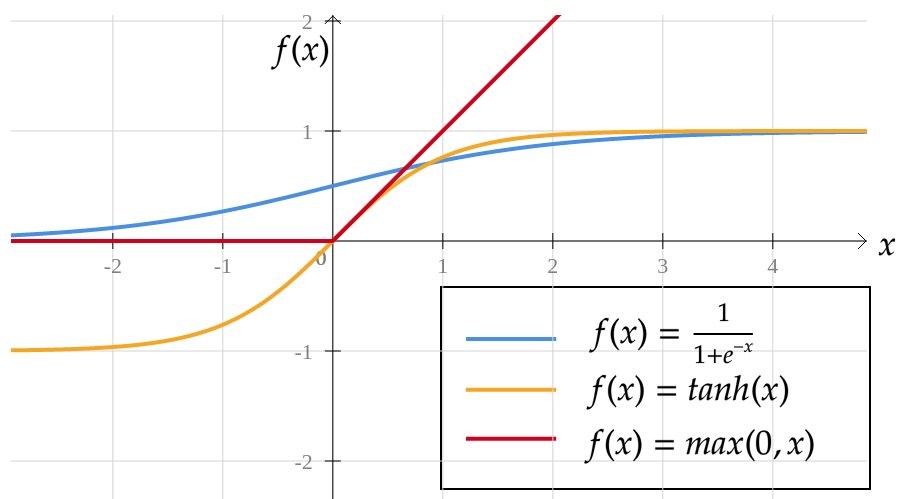
\includegraphics[width=0.7\textwidth]{imagenes/graficaF.png}
	\caption{Ejemplo de algunas de las salidas de una neurona artificial. (Imagen de autoría propia)}
	\label{fig:funciones}
\end{figure}
\par Por último la salida vectorial de la red neuronal se calcula usando la siguiente ecuación:
			
\begin{equation}
	Y\ =F\left(\left( \Theta ^{k+1}\right)^{T} A^{k}\right)
\end{equation}
			
\par Al proceso que obtiene la predicción en una red neuronal se le llama \textit{feedforward}.
			
\subsubsection{Fase de entrenamiento - optimización}
			
\par La fase entrenamiento de la red neuronal consiste en modificar los pesos $\theta$ que corresponden a cada neurona, esto se hace mediante un proceso llamado \gls{backpropagation}, éste consiste en modificar los pesos de la red de modo que se minimice la función de costo, por medio de la retroalimentación de la red hasta la primera capa. Esta idea fue por primera vez concebida por \cite{rumelhart1986learning} en su artículo \textit{Learning representations by back-propagating errors}, en el cual se calculaba el error total que se veía a la salida de la red neuronal, el cual se calcula con la ecuación \ref{eq:error}
			
\begin{equation}\label{eq:error}
	E=\frac{1}{2}\sum _{c}\sum _{j}( y_{j,c} -d_{j,c})^{2}
\end{equation}
			
donde $c$ es índice sobre las muestras, $j$ es el índice sobre las unidades se salida, $y$ es el valor de salida de la red y $d$ es el valor deseado. Luego entonces si minimizamos este error el desempeño de nuestra red neuronal con respecto al problema será mejor, este error es únicamente para la última capa, para esto es necesario derivar parcialmente la función del error con respecto a los pesos de las sinapsis de entrada de cada una de las unidades, para esto podemos ver el desarrollo que hizo \cite{rumelhart1986learning} con respecto a la función sigmoidal.
			
\par Se deriva primero el error $E$ con respecto a $y_{j}$ en cada muestra $c$, por lo tanto se omite.
\begin{equation}
	\frac{\partial E}{\partial y_{j}} =y_{j} -d_{j}
\end{equation}
\par Esta parcial es únicamente para la última capa, después se verá como calcular el de las siguientes. Después se ve que con la regla de la cadena se puede tener lo siguiente:
\begin{equation}
	\frac{\partial E}{\partial x_{j}} =\frac{\partial E}{\partial y_{j}}  \frac{\partial y_{j}}{\partial x_{j}}
\end{equation}
			
En donde $y_{j}$ está dado por la función sigmoidal en este caso por lo tanto de sustituye la derivada parcial con respecto a $x_{j}$.
\begin{spreadlines}{10pt}
	\begin{alignat}{4}
		  & y_{j} =\frac{1}{1+e^{-x_{j}}}                                                         \\
		  & \frac{\partial y_{j}}{\partial x_{j}} =\frac{e^{-x_{j}}}{1+e^{-x_{j}}}                \\
		  & \frac{\partial y_{j}}{\partial x_{j}}=y_{j} (1-y_{j})                                 \\
		  & \frac{\partial E}{\partial x_{j}} =\frac{\partial E}{\partial y_{j}}  y_{j}( 1-y_{j}) 
	\end{alignat}
\end{spreadlines}
			
\par En esta parte se puede reemplazar la parcial cuando se usa la función \gls{ReLU} o la de la tangente hiperbólica. Después se puede hacer de nuevo la regla de la cadena para obtener la derivada parcial de error con respecto a los pesos.
			
\begin{spreadlines}{10pt}
	\begin{alignat}{3}
		  & x_{j}=\sum_{i} y_{i}\theta_{ji}                                                                                          \\ \vspace{100pt}
		  & \frac{\partial E}{\partial \theta _{ji}} =\frac{\partial E}{\partial x_{j}} \frac{\partial x_{j}}{\partial \theta _{ji}} \\
		  & \frac{\partial E}{\partial \theta _{ji}} =\frac{\partial E}{\partial x_{j}}y_{i}                                         
	\end{alignat}
\end{spreadlines}
			
\par Después para conseguir la parcial del error con respecto a $x_{j}$ se debe hacer lo siguiente:
			
\begin{spreadlines}{10pt}
	\begin{alignat}{3}
		  & \frac{\partial E}{\partial x_{j}} \frac{\partial x_{j}}{\partial y_{i}} =\frac{\partial E}{\partial x_{j}} \theta _{ji} \\
		  & \frac{\partial E}{\partial y_{j}} =\sum _{j}\frac{\partial E}{\partial x_{j}} \theta _{ji}                              
	\end{alignat}
\end{spreadlines}
			
\par Con este resultado se puede calcular progresivamente las derivadas parciales del error con respecto a los pesos, en otras palabras la razón de cambio del error con respecto a la modificación de los pesos. Lo cual nos indica hacia donde está el mínimo local. Entonces para encontrar el incremento de los pesos $\theta$ podemos aplicar la siguiente ecuación:
\[ \Delta \theta =-\epsilon \frac{\partial E}{\partial \theta }\]
			
\par En esta ecuación $\epsilon$ simboliza el coeficiente de aprendizaje el cual indica que tan rápido se avanzará hacia el mínimo local. Este valor también se puede poner en función del tiempo de modo que a medida que se acerque al valor se vuelve más pequeño el paso. Este método fue primeramente descrito por \cite{rumelhart1986learning} y tiene una desventaja muy importante, para actualizar una vez los nuevos pesos es necesario computar el error de todas las muestras, por lo tanto tardará un tiempo considerable en terminar una actualización si tenemos muchas muestras, las cuales son necesarias en la mayoría de los casos para encontrar un buen modelo que generalice el problema. 

\par Este algoritmo de optimización tendrá un gran precio computacional, para este propósito se creó el \gls{SGD} el cual para actualizar los pesos en la red neuronal se obtiene el gradiente de un conjunto aleatorio de muestras, y no es necesario computar el gradiente de todo el conjunto de datos. Sin embargo este método tiene la desventaja que no se encuentra el gradiente general que describirían todas las muestras, sino una aproximación, por lo que el coeficiente de aprendizaje debe ser más pequeño y deberán hacerse más actualizaciones.

\par Otra opción que surgió con el tiempo fue dotar al cambio de los pesos de un momento esto para que aún cuando había encontrado un mínimo local, el paso pudiera pasarlo por alto con la intención de buscar uno que estuviera en la vecindad, este método no resultó tan bueno ya que podía estancarse en zonas llanas aún más altas que el mínimo local que había ignorado. Luego de este método surgió otro que consideraría una adaptación a las condiciones del gradiente, es decir que en zonas donde fuera necesario que $\epsilon$ fuera más pequeño para conseguir converger, pudiera adaptarse, entonces surgió Adagrad. Luego se pensó que se podría hacer variar de igual modo el momento ese fue el surgimiento de Adam, el cual es el método usado en esta tesis, no se pensó en probar con otros ya que Adam ha reportado mejores resultados en la literatura que sus alternativas, este método fue ideado por \cite{kingma2014adam}.  Sin embargo, como se ha visto en diferentes investigaciones, los mejores resultados se obtienen al usar como optimizador el Root Mean Square(RMS) el cual es un Gradient Descent con momento.
\nocite{DBLP:journals/corr/Ruder16}
% 			Aqui tal vez tenga que meter la explicación de Adam http://ruder.io/optimizing-gradient-descent/index.html#adam
			
\subsubsection{Éxito del método}
			
\par Las redes neuronales han sido ocupadas para muchas aplicaciones hoy en día, sin embargo en sus inicios en 1943 cuando \cite{mcculloch1943logical} investigaba como guardaba información no se pensaba que sería tan utilizado, fue con \cite{rosenblatt1958perceptron} 15 años después cuando apenas se vería un avance significativo con respecto a lo son hoy día, incluso se construyeron proyectos como Mark 1 perceptron. Sin embargo los proyectos que llegaban a ver la luz, apenas podían distinguir entre clases y con un desempeño precario, debido principalmente al poder de computo que es necesario para entrenarlas, fue más bien a partir de los años 2000 con la entrada al mercado y el desarrollo de las API por parte de NVIDIA, AMD e INTEL que la investigación comenzó a tomar el impulso que necesitaba, ahora existen muchas API de desarrollo de sistemas inteligentes como Keras, Tensorflow, Sklearn, etc. con un continuo crecimiento. Hoy en día las redes neuronales son el algoritmo número uno bio-inspirado que los investigadores usan para hacer sus experimentos (63.04\% en el 2016). Como lo menciona \cite{kar2016bio} existen muchos más algoritmos que se pueden explorar más como Artificial Plant Optimization, pero aún por mucho tiempo se prevé que las redes neuronales controlen el mercado y las investigaciones científicas gracias a que aportan resultados confiables y de rápido desarrollo sin la necesidad de conocer rigurosamente las matemáticas detrás de ellas. 
			
\par Entre los usos que se les han dado están los siguientes: en el artículo \textit{Performance Analysis of Domestic Refrigerator Using Hydrocarbon Refrigerant Mixtures with ANN} de \cite{reddy2019performance} lo usan para analizar el rendimiento de un refrigerador usando diferentes refrigerantes, en el artículo \textit{Assessing the culture of fruit farmers from Calvillo, Aguascalientes, Mexico with an artificial neural network: An approximation of sustainable land management} de \cite{santos2019assessing} se buscan soluciones para el cultivo sustentable en la región de Calvillo en Aguascalientes, en el artículo \textit{LED color prediction using a boosting neural network model for a visual-MIMO system} de \cite{banik2018led} se usa un modelo de red neuronal que predice el color de un LED, entre otras. 
			
\subsubsection{Bi-directional Long Short Term Memory}
			
\par Como se vio en la sección anterior las redes neuronales han servido ampliamente a muchas áreas del conocimiento, sin embargo para cada uno de los problemas se debe usar una arquitectura de red neuronal que sea apropiada y que se justifique que puede resolver el problema. Esta arquitectura no siempre es fácil encontrarla y muchas veces es necesario probar con más de una arquitectura con el fin de comparar resultados y decidirse por una. En otros casos es necesario utilizar modelos de forma secuencial de manera que la salida de uno sea la entrada de otro, como se puede ver, no existe nada escrito en cuanto al diseño que debe tener un modelo para resolver determinado problema. A continuación se explicará un poco sobre la arquitectura que se uso en nuestro problema y la justificación que se tuvo en mente.
            
\par Para explicar una \gls{bi-lstm} primero debemos abordar ¿Qué es una red neuronal recurrente?¿Qué es una LSTM?
            
\par Una red neuronal recurrente es una red neuronal cuyas neuronas tienen una entrada secuencial, por ejemplo una serie de palabras, una serie de caracteres, de imágenes etc. Lo que se busca con esta arquitectura es que las neuronas tengan una forma de retener información sobre los datos que han sido vistos, por lo que se puede decir que posee la capacidad de tener memoria, el modelo de esa neurona es el siguiente:
            
\begin{figure}[H]
	\centering
	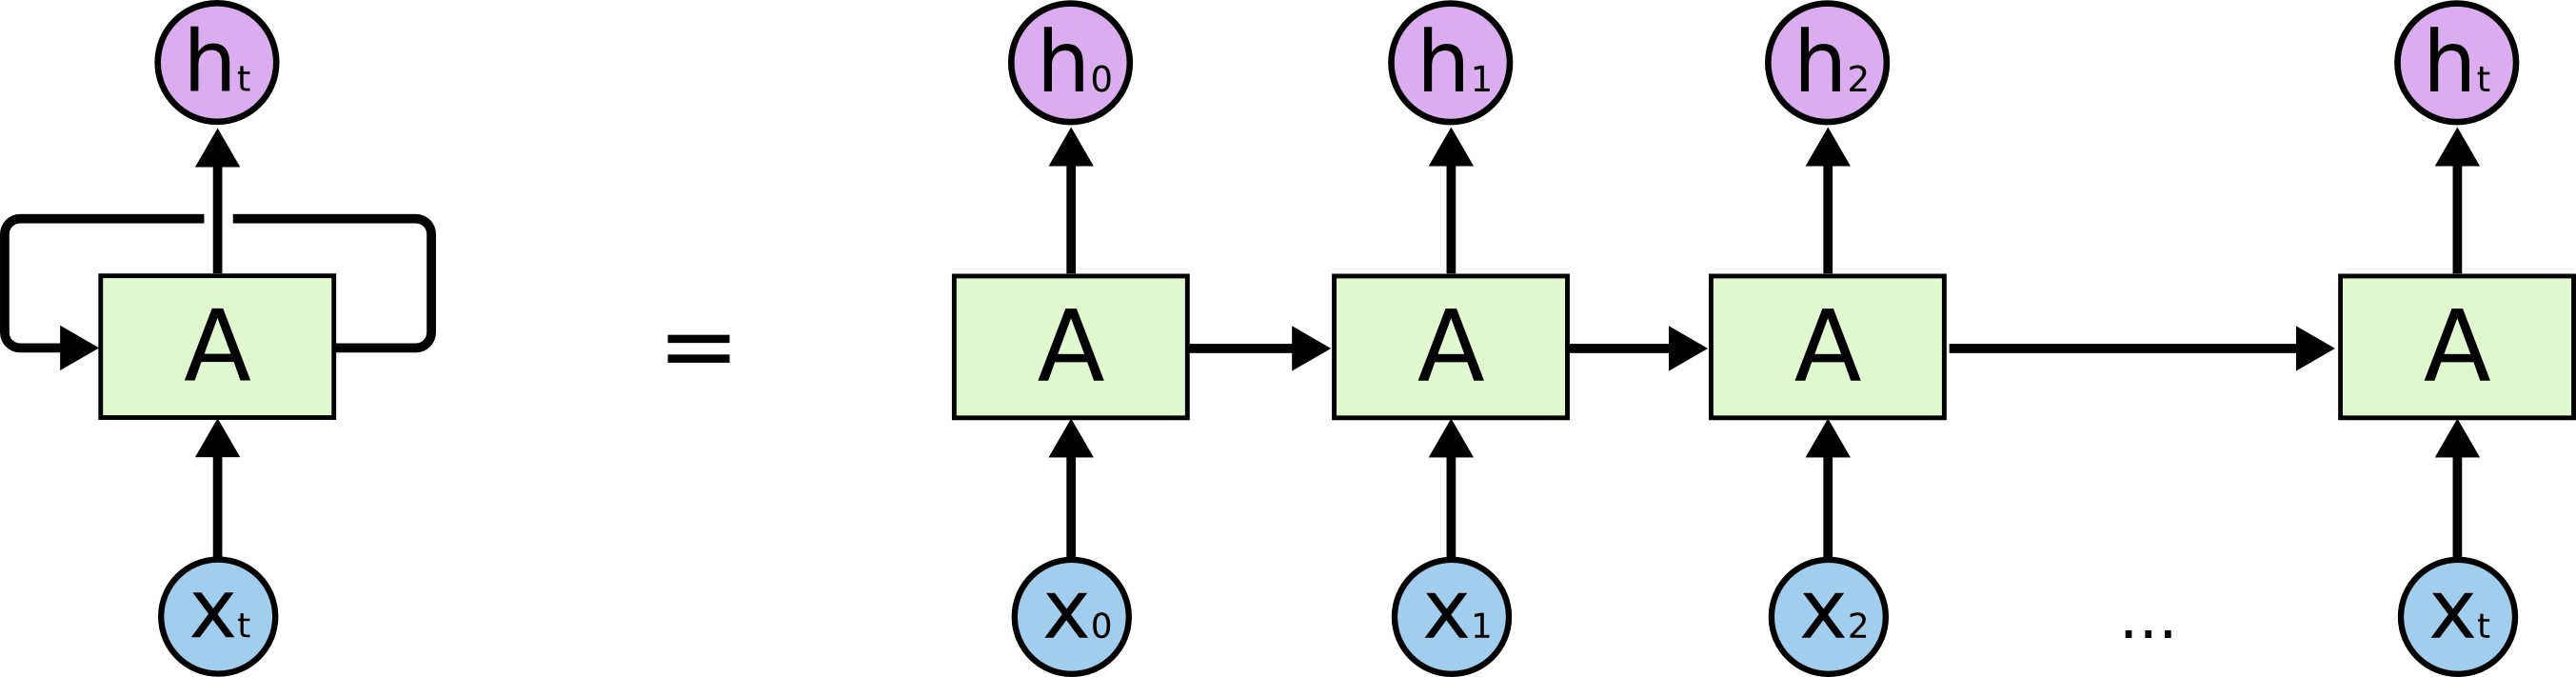
\includegraphics[width=\textwidth]{imagenes/RNN-unrolled.png}
	\caption[]{Modelo de una red neuronal recurrente. (Imagen extraída de \cite{christopher_olah_2015}) }
\end{figure}
            
\par El problema principal de que las neuronas guarden toda la información de lo que han visto es que en muchos casos es mucho más relevante la información actual que todo lo que se ha visto anteriormente, por ejemplo si en nuestro conjunto de muestras tenemos un tweet que contiene lo siguiente:
\vspace{5pt}
\begin{center}
	\textit{``Ayer me desperté temprano para ir a trabajar y cuando llegué ahí me dí cuenta que era sábado, de regreso a mi casa se me recargo una señora en el metro, gracias reloj \#thanks''}, 
	\label{fig:frase}
\end{center}
\vspace{5pt}
            
\par En este texto se puede ver que si la red neuronal esta recordando todo lo que ve, entonces ésta ``considera'' que para identificar algo como sarcasmo es igual de relevante la parte en la que se le recargo una señora que haber ido a su empleo en su día de descanso. Para dicha tarea en la que la información puede o no ser relevante se tiene la \gls{lstm} la cuales tiene una estructura similar a la siguiente:
            
\begin{figure}[H]
	\centering
	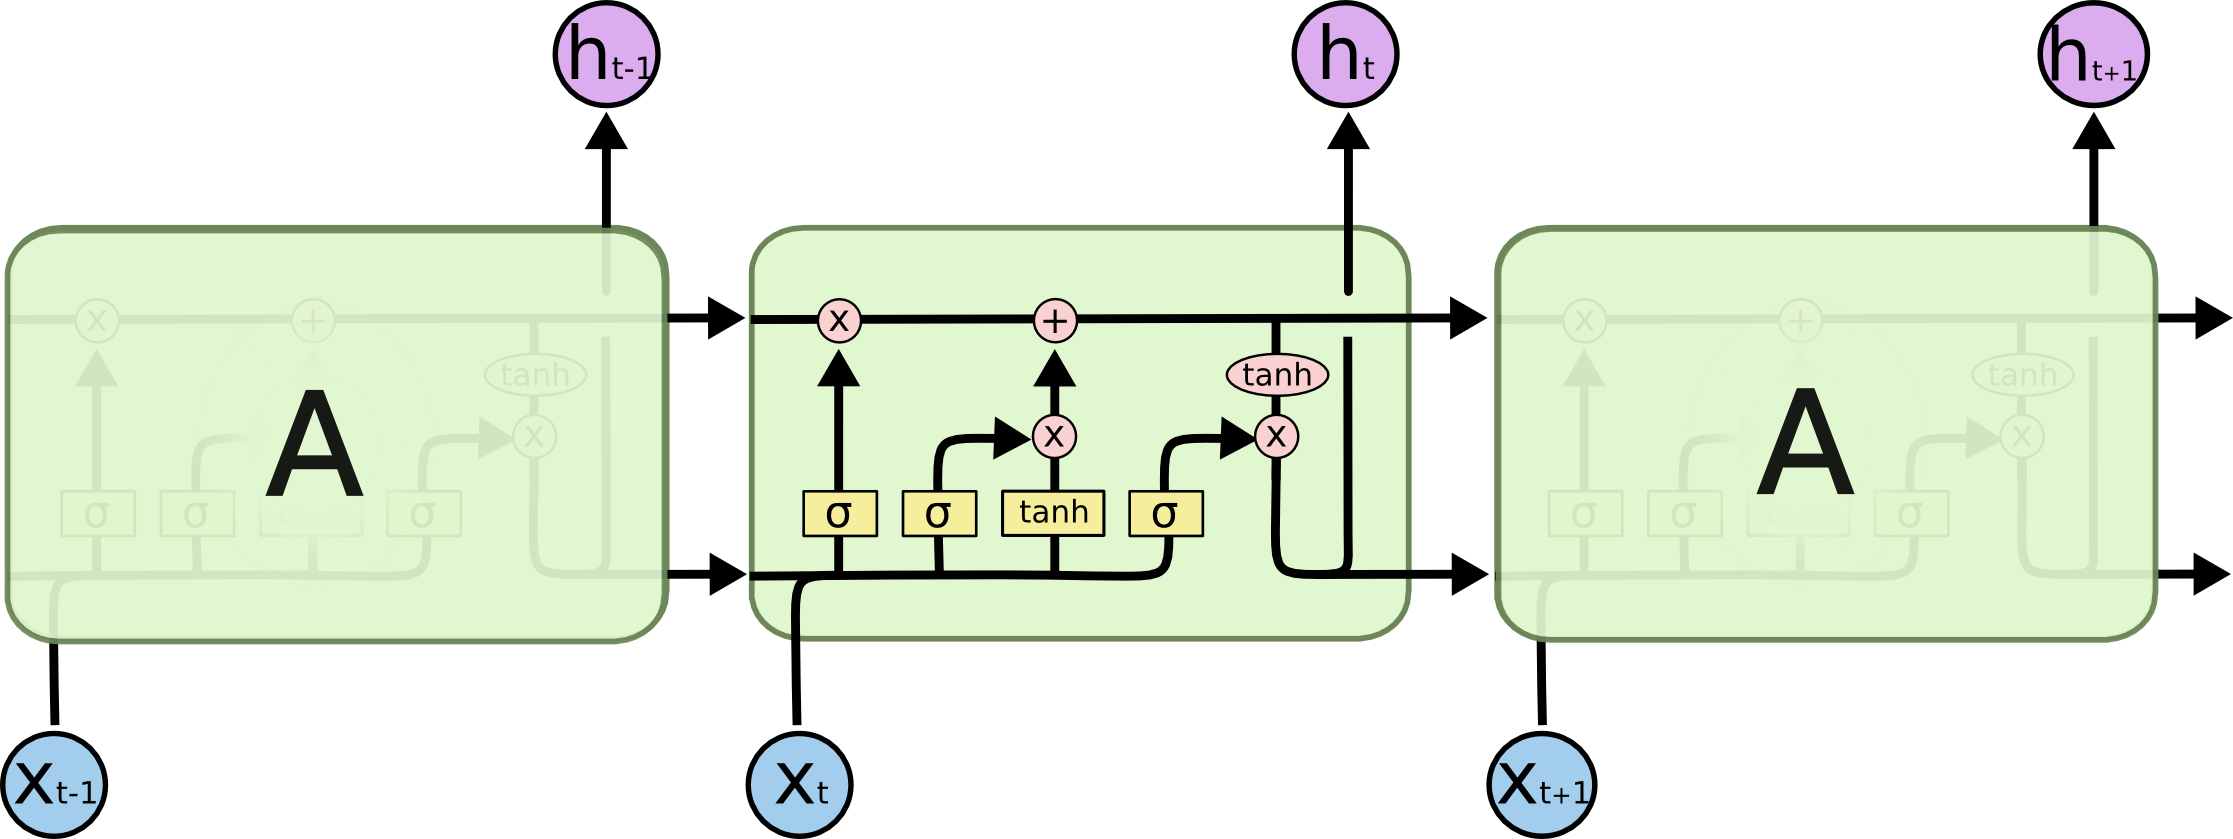
\includegraphics[width=\textwidth]{imagenes/LSTM3-chain.png}
	\caption[]{Arquitectura de una \gls{lstm}. (Imagen extraída de \cite{christopher_olah_2015})}
\end{figure}
            
            
\par Esta arquitectura tiene diferentes partes, dentro de las cuales se pueden distinguir las siguientes: la parte que decide si olvidar o no, la parte que añade el concepto actual al concepto acumulado y la parte que pasa los parámetros de salida a la entrada de la siguiente unidad. 
           
\begin{figure}[H]
	\centering
	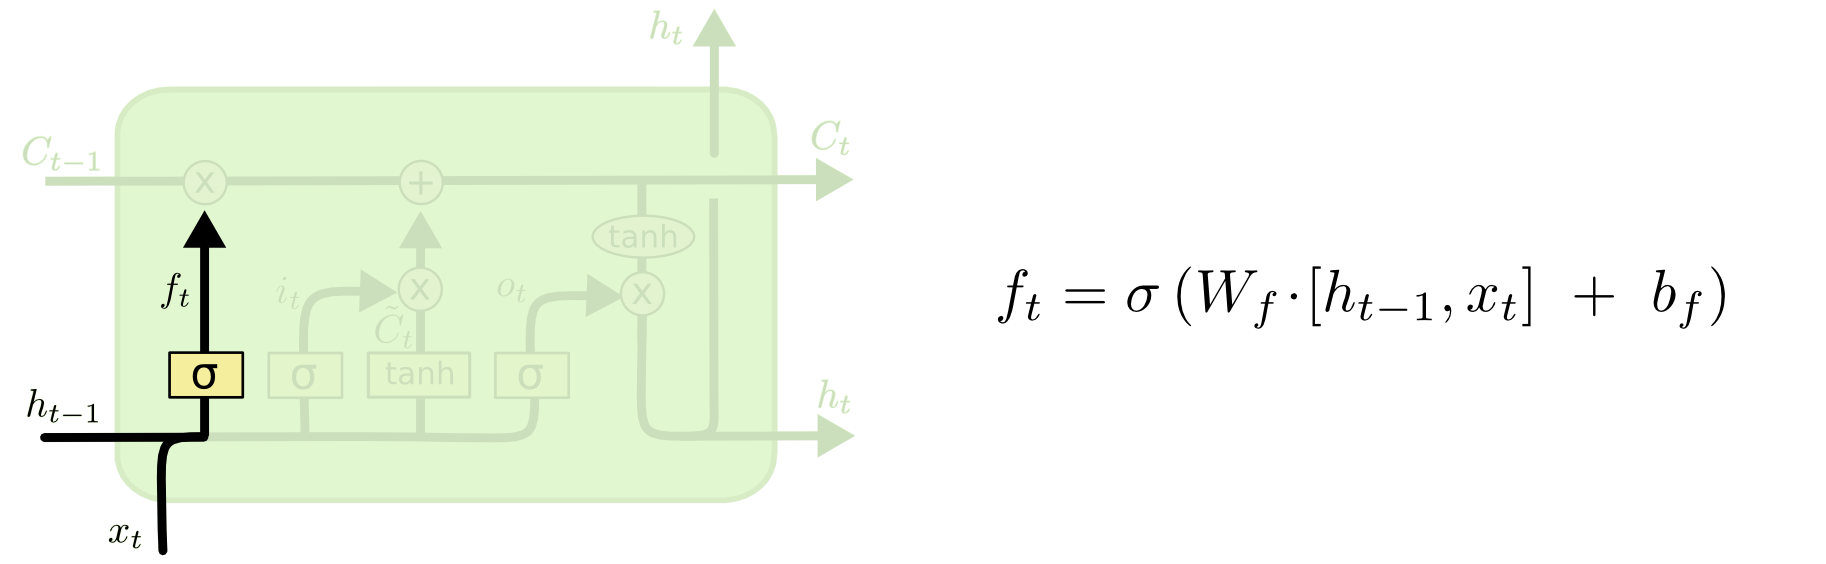
\includegraphics[width=\textwidth]{imagenes/LSTM3-focus-f.png}
	\caption[]{Sección de la unidad \gls{lstm} que decide si olvida o no.(Imagen extraída de \cite{christopher_olah_2015})}
	\label{fig:lstmOlvidar}
\end{figure}
           
           
\par En la figura \ref{fig:lstmOlvidar} $\sigma$ es la función sigmoidal que recibe la concatenación del valor que le aporta la unidad anterior y la información que actualmente puede ver, y tiene el propósito de pasar a la unidad que multiplica un valor cercano a 1, que indica que recordará todo lo que ha visto, o un valor 0 para borrar completamente lo que había visto. 
           
\begin{figure}[H]
	\centering
	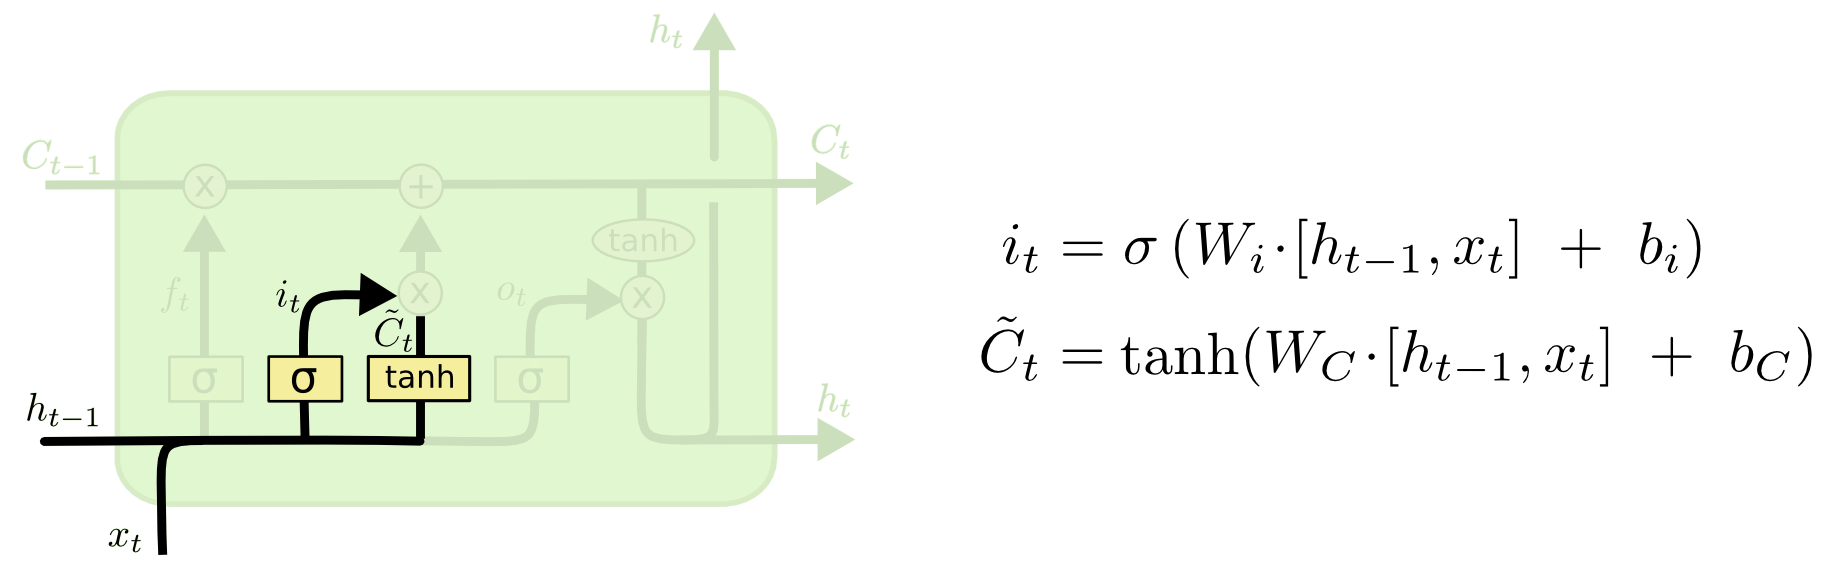
\includegraphics[width=\textwidth]{imagenes/LSTM3-focus-i.png}
	\caption[]{Sección que decide que valores del vector resumen se actualizarán. (Imagen extraída de \cite{christopher_olah_2015})}
	\label{fig:lstmAnadir}
\end{figure}

           
\par En la figura \ref{fig:lstmAnadir} se puede ver como se crean dos vectores uno $\widetilde{C_t}$ y $i_t$ los cuales simbolizan respectivamente los valores candidatos para el resumen y una máscara que filtrará los valores que la red neuronal, después de la retroalimentación, considere importantes. El filtro se aplica cuando se pasa por la unidad que multiplica. 
           
\begin{figure}[H]
	\centering
	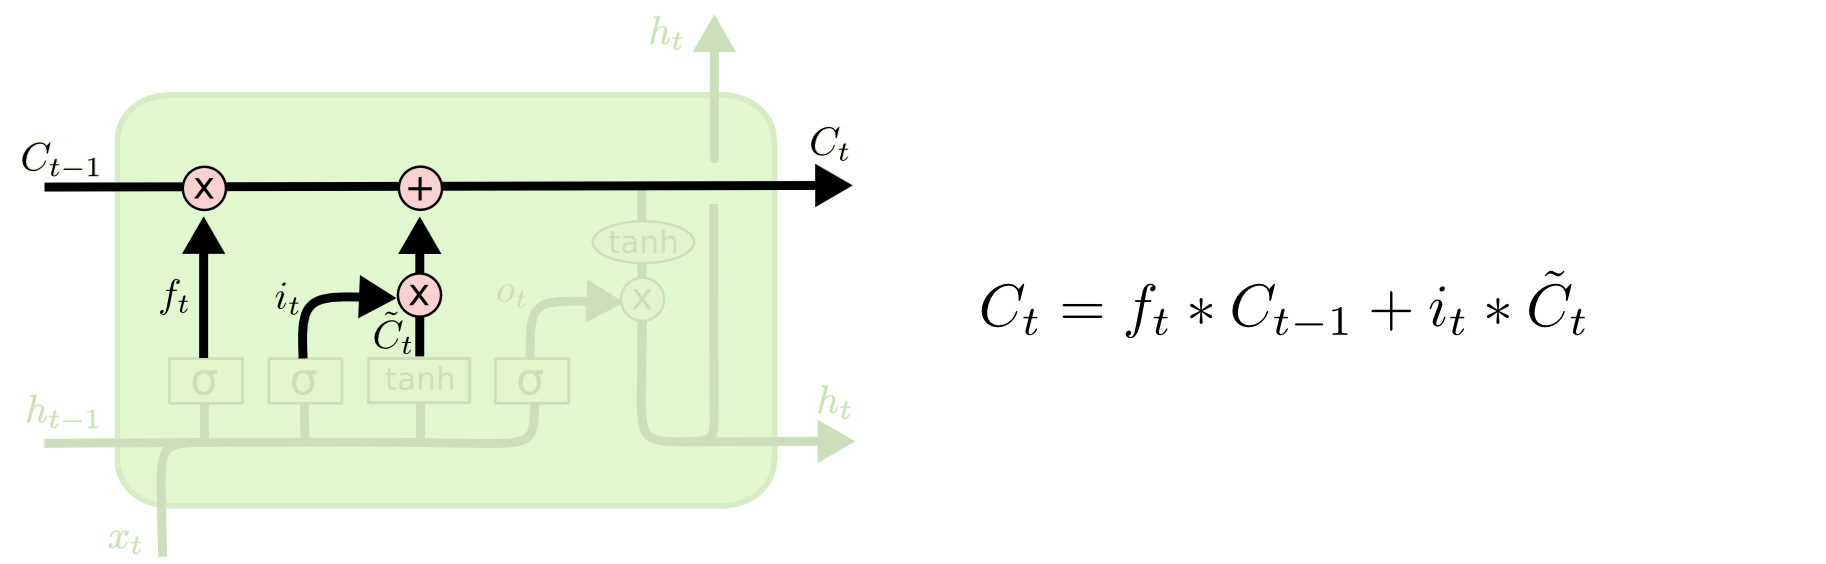
\includegraphics[width=\textwidth]{imagenes/LSTM3-focus-C.png}
	\caption[]{Sección que toma los valores que genera el conocimiento que se añadirá al conocimiento anterior. (Imagen extraída de \cite{christopher_olah_2015})}
	\label{fig:lstmSuma}
\end{figure}
           
\par En la figura \ref{fig:lstmSuma} se muestra como las entradas de una unidad cambian para convertirse en la entrada de la siguiente unidad, la unidad para multiplicar tiene el propósito de borrar la memoria de la unidad mientras que la suma tiene el propósito de añadir conocimiento a la siguiente unidad.
           
\begin{figure}[H]
	\centering
	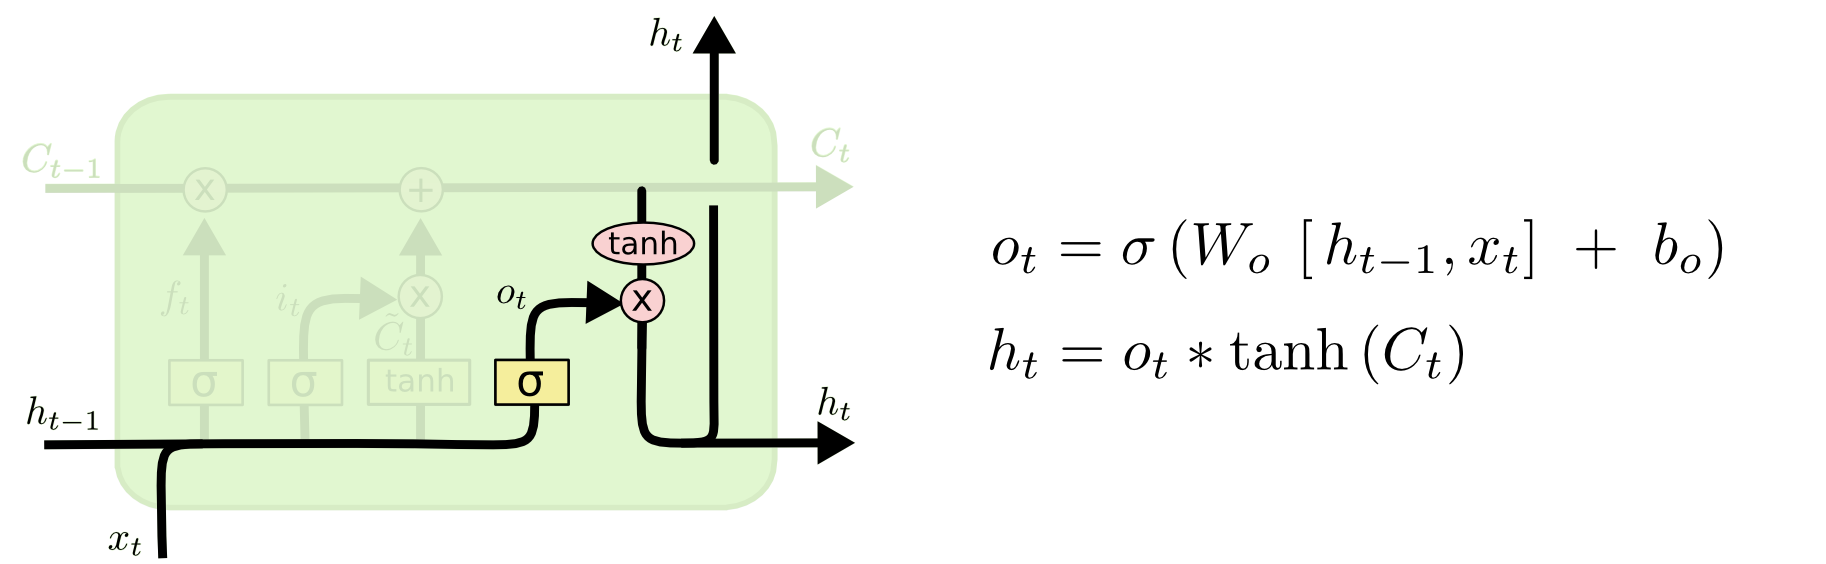
\includegraphics[width=\textwidth]{imagenes/LSTM3-focus-o.png}
	\caption[]{Sección que borra o añade el conocimiento al previo. (Imagen extraída de \cite{christopher_olah_2015})}
	\label{fig:lstmFinal}
\end{figure}
           
           
\par En la figura \ref{fig:lstmFinal} se puede ver que en la unidad se genera la salida actual de la unidad $h_t$ que también es el entrada que recibe la siguiente unidad el cual determinará si la siguiente unidad olvidará o no. 
           
\par Una \gls{bi-lstm} cambia el concepto de LSTM para encontrar la información hacia delante y hacia atrás. Añadiendo una capa que lee hacia atrás, entonces ésta se puede conecta a otra capa de red neuronal (completamente conectada) que los convierte en una salida binaria que decidirá si es irónica o no. Para que podamos ver como es la arquitectura de todo el proyecto podemos ver la figura \ref{fig:arquitectura}. 
           
\begin{landscape}
	           
	\begin{figure}
		\centering
		

\tikzset{every picture/.style={line width=0.75pt}} %set default line width to 0.75pt        

\begin{tikzpicture}[x=0.75pt,y=0.75pt,yscale=-1,xscale=1]
%uncomment if require: \path (0,560); %set diagram left start at 0, and has height of 560

%Right Arrow [id:dp8310111909351754] 
\draw  [fill={rgb, 255:red, 226; green, 122; blue, 122 }  ,fill opacity=1 ] (557,229.75) -- (607.4,229.75) -- (607.4,199) -- (641,260.5) -- (607.4,322) -- (607.4,291.25) -- (557,291.25) -- cycle ;
%Right Arrow [id:dp47914845862025834] 
\draw  [fill={rgb, 255:red, 226; green, 122; blue, 122 }  ,fill opacity=1 ] (409,229.75) -- (459.4,229.75) -- (459.4,199) -- (493,260.5) -- (459.4,322) -- (459.4,291.25) -- (409,291.25) -- cycle ;
%Shape: Rectangle [id:dp6690480869865736] 
\draw  [fill={rgb, 255:red, 186; green, 235; blue, 168 }  ,fill opacity=1 ] (340,125) -- (410,125) -- (410,411) -- (340,411) -- cycle ;
%Shape: Rectangle [id:dp5000001257312081] 
\draw  [fill={rgb, 255:red, 255; green, 255; blue, 255 }  ,fill opacity=1 ] (315,243) -- (436,243) -- (436,283) -- (315,283) -- cycle ;

%Shape: Rectangle [id:dp10129983649453078] 
\draw  [fill={rgb, 255:red, 252; green, 255; blue, 92 }  ,fill opacity=1 ] (488,125) -- (558,125) -- (558,411) -- (488,411) -- cycle ;
%Shape: Rectangle [id:dp5417230650141682] 
\draw  [fill={rgb, 255:red, 255; green, 255; blue, 255 }  ,fill opacity=1 ] (463,243) -- (584,243) -- (584,283) -- (463,283) -- cycle ;

%Shape: Rectangle [id:dp3694545240809384] 
\draw  [fill={rgb, 255:red, 105; green, 221; blue, 209 }  ,fill opacity=1 ] (638,125) -- (708,125) -- (708,411) -- (638,411) -- cycle ;
%Shape: Rectangle [id:dp46595094502729073] 
\draw  [fill={rgb, 255:red, 255; green, 255; blue, 255 }  ,fill opacity=1 ] (613,243) -- (734,243) -- (734,283) -- (613,283) -- cycle ;

%Shape: Rectangle [id:dp8981854115946217] 
\draw  [fill={rgb, 255:red, 255; green, 255; blue, 255 }  ,fill opacity=1 ] (100,54) -- (185,54) -- (185,132) -- (100,132) -- cycle ;
%Shape: Rectangle [id:dp3678809591192025] 
\draw  [fill={rgb, 255:red, 255; green, 255; blue, 255 }  ,fill opacity=1 ] (110,64) -- (195,64) -- (195,142) -- (110,142) -- cycle ;
%Shape: Rectangle [id:dp18627809361061853] 
\draw  [fill={rgb, 255:red, 255; green, 255; blue, 255 }  ,fill opacity=1 ] (120,74) -- (205,74) -- (205,152) -- (120,152) -- cycle ;

%Shape: Rectangle [id:dp5391508691442917] 
\draw  [fill={rgb, 255:red, 224; green, 224; blue, 224 }  ,fill opacity=1 ] (100,243) -- (230,243) -- (230,283) -- (100,283) -- cycle ;

%Straight Lines [id:da3222212402232878] 
\draw [color={rgb, 255:red, 226; green, 122; blue, 122 }  ,draw opacity=1 ][line width=2.25]    (230,263) -- (311,263) ;
\draw [shift={(315,263)}, rotate = 180] [fill={rgb, 255:red, 226; green, 122; blue, 122 }  ,fill opacity=1 ][line width=2.25]  [draw opacity=0] (14.29,-6.86) -- (0,0) -- (14.29,6.86) -- cycle    ;

%Shape: Circle [id:dp5889762673635599] 
\draw  [fill={rgb, 255:red, 224; green, 166; blue, 226 }  ,fill opacity=1 ] (785,167) .. controls (785,153.19) and (796.19,142) .. (810,142) .. controls (823.81,142) and (835,153.19) .. (835,167) .. controls (835,180.81) and (823.81,192) .. (810,192) .. controls (796.19,192) and (785,180.81) .. (785,167) -- cycle ;
%Shape: Circle [id:dp18063293168467354] 
\draw  [fill={rgb, 255:red, 224; green, 166; blue, 226 }  ,fill opacity=1 ] (785,338) .. controls (785,324.19) and (796.19,313) .. (810,313) .. controls (823.81,313) and (835,324.19) .. (835,338) .. controls (835,351.81) and (823.81,363) .. (810,363) .. controls (796.19,363) and (785,351.81) .. (785,338) -- cycle ;
%Straight Lines [id:da9689497769272035] 
\draw [color={rgb, 255:red, 226; green, 122; blue, 122 }  ,draw opacity=1 ][line width=2.25]    (734,257) -- (783.03,170.48) ;
\draw [shift={(785,167)}, rotate = 479.54] [fill={rgb, 255:red, 226; green, 122; blue, 122 }  ,fill opacity=1 ][line width=2.25]  [draw opacity=0] (14.29,-6.86) -- (0,0) -- (14.29,6.86) -- cycle    ;

%Straight Lines [id:da9360660330658093] 
\draw [color={rgb, 255:red, 226; green, 122; blue, 122 }  ,draw opacity=1 ][line width=2.25]    (734,257) -- (782.87,334.62) ;
\draw [shift={(785,338)}, rotate = 237.8] [fill={rgb, 255:red, 226; green, 122; blue, 122 }  ,fill opacity=1 ][line width=2.25]  [draw opacity=0] (14.29,-6.86) -- (0,0) -- (14.29,6.86) -- cycle    ;

%Straight Lines [id:da7770649855526097] 
\draw [color={rgb, 255:red, 226; green, 122; blue, 122 }  ,draw opacity=1 ][line width=2.25]    (159,152) -- (159,240) ;
\draw [shift={(159,244)}, rotate = 270] [fill={rgb, 255:red, 226; green, 122; blue, 122 }  ,fill opacity=1 ][line width=2.25]  [draw opacity=0] (14.29,-6.86) -- (0,0) -- (14.29,6.86) -- cycle    ;


% Text Node
\draw (375,264) node  [align=left] {{\Large Embedding}\\};
% Text Node
\draw (523,264) node  [align=left] {{\Large BI-LSTM}\\};
% Text Node
\draw (673,264) node  [align=left] {{\Large Dense}\\};
% Text Node
\draw (375,271) node  [align=left] {$\displaystyle |V|=$128};
% Text Node
\draw (523,272) node  [align=left] {64 unidades};
% Text Node
\draw (676,274) node  [align=left] {1 unidad};
% Text Node
\draw (162.5,113) node  [align=left] {{\fontfamily{pcr}\selectfont Tweets}};
% Text Node
\draw (165,262) node  [align=left] {Función Map\\y padding};
% Text Node
\draw (810,167) node  [align=left] {1};
% Text Node
\draw (810,337) node  [align=left] {0};
% Text Node
\draw (810,124) node  [align=left] {Irónico};
% Text Node
\draw (817,380) node  [align=left] {No irónico};


\end{tikzpicture}

		\caption{En esta figura se puede ver como es la arquitectura general del modelo que se plantea, primero de los textos extraídos de Twitter se pasan por una función de mapeo que convierte el texto en vectores, estos vectores pueden tener tener diferentes longitudes, por lo que pasa por un \gls{padding} que regulariza su longitud, después pasa al embedding que tiene como salida vectores de 128 dimensiones, estos a su vez pasan a la capa de BI-LSTM que 64 a su salida un vector de 64 unidades, las cuales pasan a una única neurona con salida binaria, la cual indica si el texto que entró es irónico o no.}
		\label{fig:arquitectura}
	\end{figure}
\end{landscape}
%aqui me quedo estoy revisando lo que escribio colah sobre esto, http://colah.github.io/posts/2015-08-Understanding-LSTMs/
%aqui explico que son las redes neuronales profundas
		
\section{Técnica de evaluación}
	
\par Una de las partes fundamentales de los modelos de inteligencia es la evaluación, en este proceso se mide de manera cuantitativa como se desempeña un sistema. Para esto existen diferentes métricas para cuantificar este desempeño. Para este experimento se usaron \textit{precision}, \textit{recall} y \textit{F-score}. 
	
\subsection{Precision}
	
\par La \textit{precision} o precisión en español se refiere a una medida de desempeño que se usa principalmente en tareas no balanceadas, esta medida trata de reconocer cuantas predicciones positivas fueron correctas entre el total de las respuesta correctas, esto se refiere principalmente a que tan bien funciona nuestro modelo en detectar nuestras muestras relevantes(en este caso las positivas). La fórmula es la siguiente: 
\begin{figure}[H]
    \centering
    \begin{equation*}
        Precision\ =\ \frac{TP}{TP+FP}    
    \end{equation*}
        \caption*{TP = True positive (muestras que se predicen positivas y que lo son) , FP = False Positive(muestras que se predicen negativas y que lo son)}
\end{figure}


\subsection{Recall}

\par El \textit{recall} o reclamo en español se refiere a la medida de desempeño de un modelo que igual que la precisión se usa en tareas con datos no balanceados. Su interpretación índica cual es la porción de muestras que se predicen positivas y lo son, entre el total de las muestras que son positivas, su fórmula es la siguiente:
	
	\begin{figure}[H]
    \centering
    \begin{equation*}
        Recall\ =\ \frac{TP}{P}\ =\ \frac{TP}{TP+FN}    
    \end{equation*}
        \caption*{TP = True positive (muestras que se predicen positivas y que lo son) , FP = False Positive(muestras que se predicen negativas y que lo son), P total de medidas que son positivas}
\end{figure}
	
\subsection{F-score}	

\par El \textit{F-Score} es una medida del desempeño que combina el \textit{recall} y el \textit{precision}, para obtener la media armónica, esto es por que las dos esta relacionadas y si una sube la otra baja. Lo importante es tener un equilibrio el cual haría el \textit{f-score} más grande. Una media armónica que trata de no sesgar el resultado de la media al valor más grande sino al mas bajo. La fórmula del f-score es la siguiente:

	\begin{figure}[H]
    \centering
    \begin{equation*}
        F-score\ =\ 2 \times  \frac{precision*recall}{precision\ +recall}
    \end{equation*}
\end{figure}
	
\subsection{Descripción de la forma de evaluación cruzada}
		
\par Para la forma de evaluación el corpus se subdividió en 5 partes del 20\% cada una, de las cuales se formaron 5 distribuciones del corpus, esto se puede ver mejor en la figura \ref{fig:corpusDiv}. 

\begin{figure}
    \centering
    

\tikzset{every picture/.style={line width=0.75pt}} %set default line width to 0.75pt        

\begin{tikzpicture}[x=0.75pt,y=0.75pt,yscale=-1,xscale=1]
%uncomment if require: \path (0,403); %set diagram left start at 0, and has height of 403

%Shape: Rectangle [id:dp4324979495520729] 
\draw  [fill={rgb, 255:red, 250; green, 240; blue, 111 }  ,fill opacity=1 ] (421.25,41.75) -- (421.25,108.25) -- (363.25,108.25) -- (363.25,41.75) -- cycle ;
%Shape: Rectangle [id:dp4732661957682942] 
\draw  [fill={rgb, 255:red, 250; green, 240; blue, 111 }  ,fill opacity=1 ] (479.25,41.75) -- (479.25,108.25) -- (421.25,108.25) -- (421.25,41.75) -- cycle ;
%Shape: Rectangle [id:dp09264088763089329] 
\draw  [fill={rgb, 255:red, 250; green, 240; blue, 111 }  ,fill opacity=1 ] (363.25,41.75) -- (363.25,108.25) -- (305.25,108.25) -- (305.25,41.75) -- cycle ;
%Shape: Rectangle [id:dp27681985257611963] 
\draw  [fill={rgb, 255:red, 250; green, 240; blue, 111 }  ,fill opacity=1 ] (305.25,41.75) -- (305.25,108.25) -- (247.25,108.25) -- (247.25,41.75) -- cycle ;
%Shape: Rectangle [id:dp35774533585505663] 
\draw  [fill={rgb, 255:red, 250; green, 240; blue, 111 }  ,fill opacity=1 ] (247.25,41.75) -- (247.25,108.25) -- (189.25,108.25) -- (189.25,41.75) -- cycle ;
%Shape: Rectangle [id:dp6300651561593915] 
\draw  [fill={rgb, 255:red, 177; green, 252; blue, 95 }  ,fill opacity=1 ] (125.31,284.39) -- (95.44,284.39) -- (95.44,258.34) -- (125.31,258.34) -- cycle ;
%Shape: Rectangle [id:dp8765465889393704] 
\draw  [fill={rgb, 255:red, 248; green, 189; blue, 72 }  ,fill opacity=1 ] (125.31,310.44) -- (95.44,310.44) -- (95.44,284.39) -- (125.31,284.39) -- cycle ;
%Shape: Rectangle [id:dp27508771757617656] 
\draw  [fill={rgb, 255:red, 177; green, 252; blue, 95 }  ,fill opacity=1 ] (125.31,258.34) -- (95.44,258.34) -- (95.44,232.29) -- (125.31,232.29) -- cycle ;
%Shape: Rectangle [id:dp9828530985786075] 
\draw  [fill={rgb, 255:red, 177; green, 252; blue, 95 }  ,fill opacity=1 ] (125.31,232.29) -- (95.44,232.29) -- (95.44,206.24) -- (125.31,206.24) -- cycle ;
%Shape: Rectangle [id:dp8511798847882142] 
\draw  [fill={rgb, 255:red, 177; green, 252; blue, 95 }  ,fill opacity=1 ] (125.31,206.24) -- (95.44,206.24) -- (95.44,180.19) -- (125.31,180.19) -- cycle ;
%Shape: Rectangle [id:dp24215577820153578] 
\draw  [fill={rgb, 255:red, 248; green, 189; blue, 72 }  ,fill opacity=1 ] (235.31,284.39) -- (205.44,284.39) -- (205.44,258.34) -- (235.31,258.34) -- cycle ;
%Shape: Rectangle [id:dp20025071615226597] 
\draw  [fill={rgb, 255:red, 177; green, 252; blue, 95 }  ,fill opacity=1 ] (235.31,310.44) -- (205.44,310.44) -- (205.44,284.39) -- (235.31,284.39) -- cycle ;
%Shape: Rectangle [id:dp8410616935900397] 
\draw  [fill={rgb, 255:red, 177; green, 252; blue, 95 }  ,fill opacity=1 ] (235.31,258.34) -- (205.44,258.34) -- (205.44,232.29) -- (235.31,232.29) -- cycle ;
%Shape: Rectangle [id:dp9019405855389522] 
\draw  [fill={rgb, 255:red, 177; green, 252; blue, 95 }  ,fill opacity=1 ] (235.31,232.29) -- (205.44,232.29) -- (205.44,206.24) -- (235.31,206.24) -- cycle ;
%Shape: Rectangle [id:dp8723175446401576] 
\draw  [fill={rgb, 255:red, 177; green, 252; blue, 95 }  ,fill opacity=1 ] (235.31,206.24) -- (205.44,206.24) -- (205.44,180.19) -- (235.31,180.19) -- cycle ;
%Shape: Rectangle [id:dp10475735860334345] 
\draw  [fill={rgb, 255:red, 177; green, 252; blue, 95 }  ,fill opacity=1 ] (345.31,284.39) -- (315.44,284.39) -- (315.44,258.34) -- (345.31,258.34) -- cycle ;
%Shape: Rectangle [id:dp8360710594149254] 
\draw  [fill={rgb, 255:red, 177; green, 252; blue, 95 }  ,fill opacity=1 ] (345.31,310.44) -- (315.44,310.44) -- (315.44,284.39) -- (345.31,284.39) -- cycle ;
%Shape: Rectangle [id:dp3251826315662174] 
\draw  [fill={rgb, 255:red, 248; green, 189; blue, 72 }  ,fill opacity=1 ] (345.31,258.34) -- (315.44,258.34) -- (315.44,232.29) -- (345.31,232.29) -- cycle ;
%Shape: Rectangle [id:dp43410729341495813] 
\draw  [fill={rgb, 255:red, 177; green, 252; blue, 95 }  ,fill opacity=1 ] (345.31,232.29) -- (315.44,232.29) -- (315.44,206.24) -- (345.31,206.24) -- cycle ;
%Shape: Rectangle [id:dp2237354541869716] 
\draw  [fill={rgb, 255:red, 177; green, 252; blue, 95 }  ,fill opacity=1 ] (345.31,206.24) -- (315.44,206.24) -- (315.44,180.19) -- (345.31,180.19) -- cycle ;
%Shape: Rectangle [id:dp05371800101329849] 
\draw  [fill={rgb, 255:red, 177; green, 252; blue, 95 }  ,fill opacity=1 ] (455.31,284.39) -- (425.44,284.39) -- (425.44,258.34) -- (455.31,258.34) -- cycle ;
%Shape: Rectangle [id:dp35978328802574344] 
\draw  [fill={rgb, 255:red, 177; green, 252; blue, 95 }  ,fill opacity=1 ] (455.31,310.44) -- (425.44,310.44) -- (425.44,284.39) -- (455.31,284.39) -- cycle ;
%Shape: Rectangle [id:dp11324731127997034] 
\draw  [fill={rgb, 255:red, 177; green, 252; blue, 95 }  ,fill opacity=1 ] (455.31,258.34) -- (425.44,258.34) -- (425.44,232.29) -- (455.31,232.29) -- cycle ;
%Shape: Rectangle [id:dp3713437467654701] 
\draw  [fill={rgb, 255:red, 248; green, 189; blue, 72 }  ,fill opacity=1 ] (455.31,232.29) -- (425.44,232.29) -- (425.44,206.24) -- (455.31,206.24) -- cycle ;
%Shape: Rectangle [id:dp3078959049885366] 
\draw  [fill={rgb, 255:red, 177; green, 252; blue, 95 }  ,fill opacity=1 ] (455.31,206.24) -- (425.44,206.24) -- (425.44,180.19) -- (455.31,180.19) -- cycle ;
%Shape: Rectangle [id:dp9529437202543025] 
\draw  [fill={rgb, 255:red, 177; green, 252; blue, 95 }  ,fill opacity=1 ] (565.31,284.39) -- (535.44,284.39) -- (535.44,258.34) -- (565.31,258.34) -- cycle ;
%Shape: Rectangle [id:dp9922975154494478] 
\draw  [fill={rgb, 255:red, 177; green, 252; blue, 95 }  ,fill opacity=1 ] (565.31,310.44) -- (535.44,310.44) -- (535.44,284.39) -- (565.31,284.39) -- cycle ;
%Shape: Rectangle [id:dp8226822462900152] 
\draw  [fill={rgb, 255:red, 177; green, 252; blue, 95 }  ,fill opacity=1 ] (565.31,258.34) -- (535.44,258.34) -- (535.44,232.29) -- (565.31,232.29) -- cycle ;
%Shape: Rectangle [id:dp6350529855385154] 
\draw  [fill={rgb, 255:red, 177; green, 252; blue, 95 }  ,fill opacity=1 ] (565.31,232.29) -- (535.44,232.29) -- (535.44,206.24) -- (565.31,206.24) -- cycle ;
%Shape: Rectangle [id:dp19244781197245708] 
\draw  [fill={rgb, 255:red, 248; green, 189; blue, 72 }  ,fill opacity=1 ] (565.31,206.24) -- (535.44,206.24) -- (535.44,180.19) -- (565.31,180.19) -- cycle ;
%Straight Lines [id:da9512591343165853] 
\draw [line width=2.25]    (335.5,117) -- (135.36,171.94) ;
\draw [shift={(131.5,173)}, rotate = 344.65] [fill={rgb, 255:red, 0; green, 0; blue, 0 }  ][line width=2.25]  [draw opacity=0] (16.07,-7.72) -- (0,0) -- (16.07,7.72) -- (10.67,0) -- cycle    ;

%Straight Lines [id:da04818720431299961] 
\draw [line width=2.25]    (335.5,117) -- (232.07,169.2) ;
\draw [shift={(228.5,171)}, rotate = 333.22] [fill={rgb, 255:red, 0; green, 0; blue, 0 }  ][line width=2.25]  [draw opacity=0] (16.07,-7.72) -- (0,0) -- (16.07,7.72) -- (10.67,0) -- cycle    ;

%Straight Lines [id:da5826595319338874] 
\draw [line width=2.25]    (335.5,117) -- (333.87,170.75) ;
\draw [shift={(333.75,174.75)}, rotate = 271.74] [fill={rgb, 255:red, 0; green, 0; blue, 0 }  ][line width=2.25]  [draw opacity=0] (16.07,-7.72) -- (0,0) -- (16.07,7.72) -- (10.67,0) -- cycle    ;

%Straight Lines [id:da3687801654619345] 
\draw [line width=2.25]    (335.5,117) -- (522.67,173.84) ;
\draw [shift={(526.5,175)}, rotate = 196.89] [fill={rgb, 255:red, 0; green, 0; blue, 0 }  ][line width=2.25]  [draw opacity=0] (16.07,-7.72) -- (0,0) -- (16.07,7.72) -- (10.67,0) -- cycle    ;

%Straight Lines [id:da5919916039876636] 
\draw [line width=2.25]    (335.5,117) -- (427.77,169.28) ;
\draw [shift={(431.25,171.25)}, rotate = 209.54] [fill={rgb, 255:red, 0; green, 0; blue, 0 }  ][line width=2.25]  [draw opacity=0] (16.07,-7.72) -- (0,0) -- (16.07,7.72) -- (10.67,0) -- cycle    ;

%Shape: Rectangle [id:dp3523228887868648] 
\draw  [fill={rgb, 255:red, 248; green, 189; blue, 72 }  ,fill opacity=1 ] (125.31,360.44) -- (95.44,360.44) -- (95.44,334.39) -- (125.31,334.39) -- cycle ;
%Shape: Rectangle [id:dp08317013348175117] 
\draw  [fill={rgb, 255:red, 177; green, 252; blue, 95 }  ,fill opacity=1 ] (125.31,394.39) -- (95.44,394.39) -- (95.44,368.34) -- (125.31,368.34) -- cycle ;

% Text Node
\draw (218.25,75) node  [align=left] {{\large 1}};
% Text Node
\draw (275.25,75) node  [align=left] {{\large 2}};
% Text Node
\draw (333.25,75) node  [align=left] {{\large 3}};
% Text Node
\draw (392.25,75) node  [align=left] {{\large 4}};
% Text Node
\draw (451.25,75) node  [align=left] {{\large 5}};
% Text Node
\draw (110,193) node  [align=left] {1};
% Text Node
\draw (110,221) node  [align=left] {2};
% Text Node
\draw (111,246) node  [align=left] {3};
% Text Node
\draw (111,271) node  [align=left] {4};
% Text Node
\draw (111,298) node  [align=left] {5};
% Text Node
\draw (220,193) node  [align=left] {1};
% Text Node
\draw (220,221) node  [align=left] {2};
% Text Node
\draw (221,246) node  [align=left] {3};
% Text Node
\draw (221,271) node  [align=left] {4};
% Text Node
\draw (221,298) node  [align=left] {5};
% Text Node
\draw (330,193) node  [align=left] {1};
% Text Node
\draw (330,221) node  [align=left] {2};
% Text Node
\draw (331,246) node  [align=left] {3};
% Text Node
\draw (331,271) node  [align=left] {4};
% Text Node
\draw (331,298) node  [align=left] {5};
% Text Node
\draw (440,193) node  [align=left] {1};
% Text Node
\draw (440,221) node  [align=left] {2};
% Text Node
\draw (441,246) node  [align=left] {3};
% Text Node
\draw (441,271) node  [align=left] {4};
% Text Node
\draw (441,298) node  [align=left] {5};
% Text Node
\draw (550,193) node  [align=left] {1};
% Text Node
\draw (550,221) node  [align=left] {2};
% Text Node
\draw (551,246) node  [align=left] {3};
% Text Node
\draw (551,271) node  [align=left] {4};
% Text Node
\draw (551,298) node  [align=left] {5};
% Text Node
\draw (218,349) node  [align=left] {Conjunto de evaluación};
% Text Node
\draw (231,379) node  [align=left] {Conjunto de entrenamiento};


\end{tikzpicture}

    \caption{Del corpus total se separaron 5 versiones las cuales cambian su sección de prueba y de entrenamiento, para después promediar sus puntajes.}
    \label{fig:corpusDiv}
\end{figure}

\par Sobre estos 5 grupos se entrenó el mismo clasificador usando el 80\% para entrenamiento y el 20\% para la fase de evaluación. Los datos que se ven en el capítulo \ref{cap.experimentos} se promedian y se reportan. 

\subsection{ROC y AUC}

\par Otra forma de evaluación que se realizará es la métrica ROC y AUC. Una gráfica \textit{`receiver operating characteristics (ROC)'} es un método gráfico para calificar el desempeño de un clasificador. 
\par En nuestro caso consistirá desplazar el umbral de discretización para observar como se da el aumento de los \textit{true positive rate} y \textit{false positive rate}. Esta gráfica es bastante sencilla, sin embargo su interpretación no es nada trivial, por lo que no se tratará a fondo en esta tesis.  

\begin{figure}
    \centering
    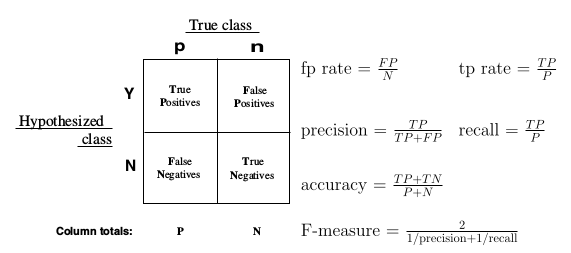
\includegraphics[width=\linewidth]{imagenes/confusionMatrix.png}
    \caption{Matriz de confusión. Imagen extraída de \cite{fawcett2006introduction}}
    \label{fig:confMat}
\end{figure}

\par Esta métrica nos ayuda a visualizar fácilmente que pasa con el comportamiento de un clasificador cuando se le cambia el umbral. Para entenderla se debe analizar una curva ROC muestra.

\begin{figure}[H]
    \centering
    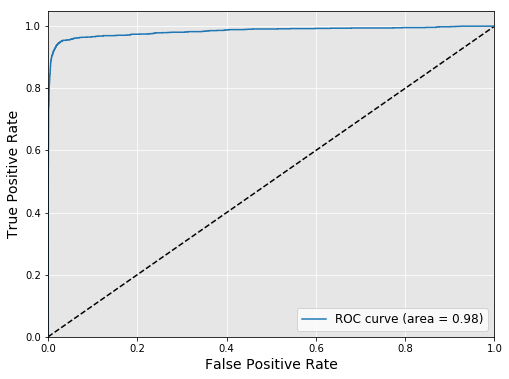
\includegraphics[width=\linewidth]{imagenes/ROC_Exp3_1.png}
    \caption{Curva ROC experimento 3}
    \label{fig:ROCMuestra}
\end{figure}

\par En \ref{fig:ROCMuestra} se puede observar una recta a \ang{45} la cual es la recta que se obtendría si se hace una clasificación aleatoria. Luego la recta azul es la recta que se obtuvo de mover el umbral de 0 a 1. Se Puede ver que cuando el umbral es 0, todas las muestras serán positivas entonces nuestro \textit{false positive rate} y el  \textit{true positive rate} aumentarán a 1 o lo que es lo mismo se tendrá un punto en (1,1). Por el lado contrario si se tiene el umbral en 1 el \textit{false positive rate} y el  \textit{true positive rate} disminuirán a 0 y se tendrá un punto en (0,0). Lo que buscamos con nuestro modelo es tener el \textit{true positive rate} en 1 y el \textit{false positive rate} en 0 o lo que es lo mismo tener un punto en (0,1). Como es muy probable que nuestro modelo tenga dicho punto, se puede considerar que entre más cerca mejor y esto se logra si tenemos bien separadas nuestras clases. Es decir, cuando tenemos una clase en un extremo de nuestro umbral y la otra del otro, de este modo el movimiento de nuestro umbral no afectará tanto en la clasificación. Esto es lo que mide la gráfica ROC.

\par Hablado ahora del \textit{area under the curve} es la reducción de la gráfica ROC a un escalar el cual es representado por el área bajo la curva, esto nos dirá que tanto nos pudimos acercar al punto deseado (0,1) y que tan estable es nuestro modelo al clasificar.

\subsection{Justificación}	

\par El \textit{recall} y el \textit{precision} son las medidas que generalmente se usan para medir el desempeño, principalmente por que aportan información sobre que tan bien realizan la tarea cuando los datos no están balanceados, lo cual sucede la mayoría de las veces. Además el \textit{f-score} nos aporta una mejor utilidad ya que aporta información de ambas medidas, sin tender a sesgar el resultado por el valor más grande sino por el más pequeño.

\par La gráfica ROC y el AUC son métodos gráficos ampliamente usado que pueden servir para rápidamente identificar si un modelo tiene un buen desempeño o no. Por lo que se considera valioso para los experimentos.

% incluir esto en la tesis
%https://en.wiktionary.org/wiki/User:Matthias_Buchmeier#Spanish_frequency_list
\chapter{Experimentos}\label{cap.experimentos}


\par El modelo propuesto de clasificación de ironía se implementó en Python. Este capítulo consiste en presentar, comparar y dar una explicación sobre por que se obtienen dichos resultados, para cada uno de los experimentos se probó con diferentes configuraciones para compararlos entre ellos, con el objetivo de encontrar la que presente mejores resultados.

\section{Primer experimento}

\par En este primer experimento se probó con una arquitectura con una primera capa de embedding de 128 unidades de salida, seguida de una capa \gls{bi-lstm} de 200 unidades, después una capa de dropout con parámetro de 0.5, seguida de una capa completamente conectada con una única salida que representa el resultado binario que indica si la oración es irónica o no. Este experimento se distingue de los demás ya que no tomamos en cuenta los caracteres especiales, únicamente el texto el cual se normaliza a ASCII con el propósito de no darle tanta importancia a la ortografía. Se agrega al final un carácter que delimita si es el final de la sentencia.

\subsection{Evaluación}
\begin{center}
	\begin{table}[h]
    \centering
    \caption{Tabla de métricas experimento 1, análisis por palabra. Nótese que la métrica con valor más alto es la exactitud, con un promedio de 0.9687; sin embargo, el recall cae debido a que no le es posible encontrar más muestras positivas, esto puede deberse a que ignora mucha información valiosa que contienen las palabras que se omiten. La desviación estándar resulta ser muy baja, lo cuál indica que este experimento no varía tanto y por lo tanto los promedios describen el comportamiento esencial del modelo.}
\begin{tabular}{|l|llll|}
\hline
              & Exactitud &     Precisión &     Recall  &   F-score \\ \hline

Subdivisión1            &       0.9698  &       0.9277  &       0.7589  &       0.8349  \\ 
Subdivisión2            &       0.9671  &       0.8422  &       0.8246  &       0.8333  \\ 
Subdivisión3            &       0.9692  &       0.9045  &       0.7720  &       0.8330  \\ 
Subdivisión4            &       0.9677  &       0.9569  &       0.7097  &       0.8150  \\ 
Subdivisión5            &       0.9698  &       0.9146  &       0.7694  &       0.8358  \\ \hline
Promedio                &       0.9687  &       0.9092  &       0.7669  &       0.8304  \\ \hline
Desviación estándar     &       0.0011  &       0.0378  &       0.0366  &       0.0078  \\ \hline

% Subdivisión 1 & 0.9709  &       0.9674  &       0.7226  &       0.8273 \\
% Subdivisión 2 & 0.9677  &       0.9529  &       0.7037  &       0.8095   \\
% Subdivisión 3 & 0.9647  &       0.9711  &       0.6793  &       0.7994   \\
% Subdivisión 4 & 0.9698  &       0.9719  &       0.7333  &       0.8359   \\
% Subdivisión 5 & 0.9722  &       0.9312  &       0.7713  &       0.8437  \\ \hline
% Promedio      & 0.9690  &       0.9589  &       0.7220  &       0.8232\\ \hline
\end{tabular}
		     \label{tab:exp1}
\end{table}
\end{center}

\par Como se puede apreciar en la tabla \ref{tab:exp1} la precisión medida sobre el modelo, es similar a la obtenida en la bibliografía, lo cual indica que este modelo se desempeña bastante bien en reconocer la ironía. Sin embargo, como se vió, el \textit{recall} es considerablemente bajo, por lo que este modelo tiende a no encontrar un gran porcentaje de las muestras irónicas. Ademá se puede ver que el \textit{F-score} es bastante similar a los de la bibliografía.

\par A continuación en la figura \ref{fig:Roc1} se muestran algunas de las gráficas ROC qué muestran qué tan bien se desempeña esta arquitectura y preprocesamiento.

\begin{figure}
	\begin{table}[H]
		\centering
		\makebox[10pt][c]{
			\begin{tabular}{cc}

				\addheight{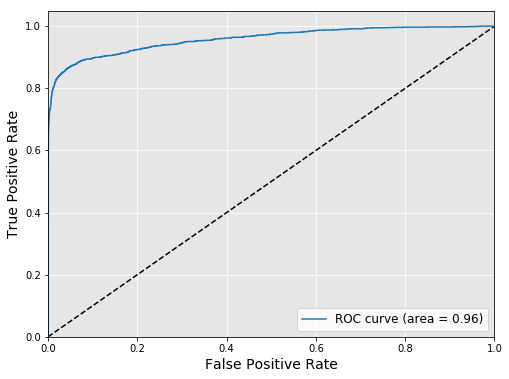
\includegraphics[width=80mm]{imagenes/ROC_Exp1_1.png}} &
				\addheight{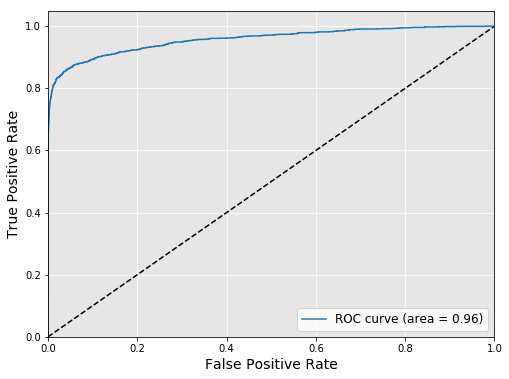
\includegraphics[width=80mm]{imagenes/ROC_Exp1_2.png}}              \\
				\small Segmento 1                                                 & Segmento 2 \\

				\addheight{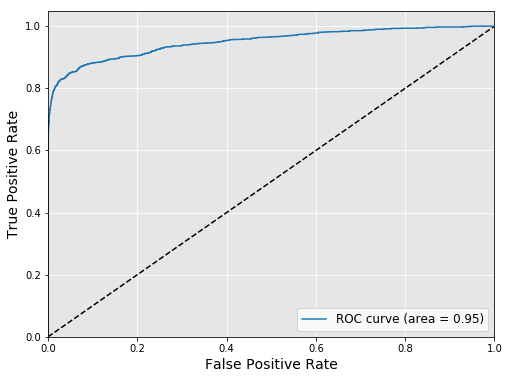
\includegraphics[width=80mm]{imagenes/ROC_Exp1_3.png}} &
				\addheight{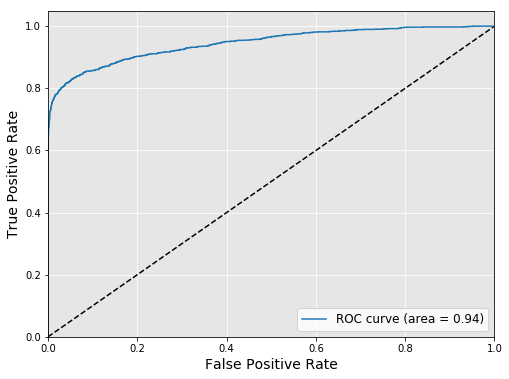
\includegraphics[width=80mm]{imagenes/ROC_Exp1_4.png}}              \\
				\small Segmento 3                                                 & Segmento 4 \\

				\addheight{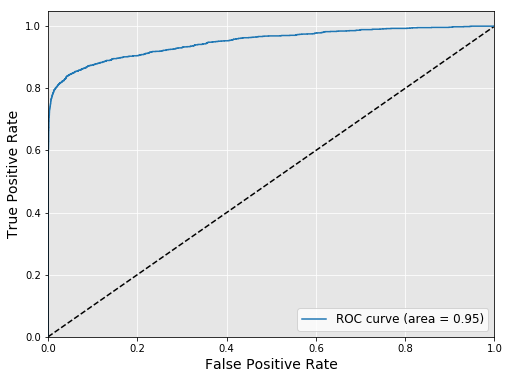
\includegraphics[width=80mm]{imagenes/ROC_Exp1_5.png}} &
				\\
				\small Segmento 5                                                 &            \\
			\end{tabular}
		}
	\end{table}
	\caption{Gráficas ROC de los segmentos en que se dividió el corpus. Primer Experimento preprocesamiento por palabra. En este experimento se puede apreciar como las gráficas ROC tiene un línea más accidentada, lo cual determina que tan estable es el modelo, si se mueve el umbral. El área bajo la curva alcanza 0.96, es un buen resultado, sin embargo, al compararlo con los demás experimentos se puede notar que no es tan relevante.}
	\label{fig:Roc1}
\end{figure}


\subsection{Propuesta de mejora}

\par Mi propuesta de mejora es que en lugar de considerar las palabras como tokens, se consideren los caracteres. Esto podría mejorar el desempeño ya que dejaríamos que la red neuronal aprendiera de la forma que escriben los usuarios y no se esforzaría tanto por encontrar correlaciones con palabras que no se encuentran en una oración. Similar a como los humanos leemos las palabras, ya que podemos extraer características diferentes de dos textos que tienen un contenido similar por ejemplo: `hola' y `holaaaaaaa' en la primera podemos notar que es ortograficamente correcta. No obstante no da mucha información por sí misma, con la segunda podemos ver que no es ortograficamente correcta, por lo que muy probablemente no este en el vocabulario que se extrajo del conjunto de entrenamiento. Si la palabra tiene los últimos caracteres repetidos puede indicar que se quiere hacer algún tipo de énfasis, o que el emisor quiere señalar algo evidente. Estos son ejemplos de características que se pueden obtener si se hace un análisis carácter por carácter y la principal motivación para el siguiente experimento.

\section{Segundo experimento}
\par En este segundo experimento se quiso cambiar el preprocesamiento, realizando lo más sencillo, pasar el tweet a una lista de caracteres y considerar cada uno como unidad de información. Entonces el vocabulario sería cada uno de los caracteres que se encuentran presentes en el corpus distinguiendo si eran mayúsculas o minúsculas. Tampoco se excluyeron los caracteres especiales, para de este modo captar la mayor información posible.
\subsection{Evaluación}
\begin{center}
	\begin{table}[h]
    \centering
    \caption{Tabla de métricas experimento 2, análisis por carácter. Se nota un mejor desempeño respecto al primer experimento, debido a que las palabras que fueron ignoradas antes, ahora aportan su información. La mejor métrica de este experimento fue la exactitud, pero se nota una mejora significativa en la precisión y en el recall, de 5 y 10 puntos porcentuales respectivamente. La desviación estándar resulta ser muy baja, lo cuál indica que este experimento no varía tanto y por lo tanto los promedios describen el comportamiento esencial del modelo. }
\begin{tabular}{|l|llll|}
\hline
                        & Exactitud &     Precisión &     Recall  &   F-score \\ \hline
              
Subdivisión1            &       0.9840  &       0.9450  &       0.8928  &       0.9181  \\ 
Subdivisión2            &       0.9842  &       0.9646  &       0.8737  &       0.9169  \\ 
Subdivisión3            &       0.9811  &       0.9477  &       0.8568  &       0.8999  \\ 
Subdivisión4            &       0.9801  &       0.9562  &       0.8402  &       0.8944  \\ 
Subdivisión5            &       0.9833  &       0.9623  &       0.8674  &       0.9124  \\ \hline
Promedio                &       0.9825  &       0.9552  &       0.8662  &       0.9084  \\ \hline
Desviación estándar     &       0.0016  &       0.0078  &       0.0175  &       0.0095  \\ \hline
              
% Subdivisión 1 & 0.9716  &       0.8911  &       0.8130  &       0.8503 \\
% Subdivisión 2 & 0.9639  &       0.8648  &       0.7557  &       0.8066   \\
% Subdivisión 3 & 0.9768  &       0.8905  &       0.8808  &       0.8857   \\
% Subdivisión 4 & 0.9660  &       0.8683  &       0.7723  &       0.8175   \\
% Subdivisión 5 & 0.9707  &       0.8894  &       0.8096  &       0.8476   \\ \hline
% Promedio      & 0.9698  &       0.8808  &       0.8063  &       0.8415\\ \hline
\end{tabular}
		     \label{tab:exp2}
\end{table}
\end{center}


\par En la tabla \ref{tab:exp2} se puede notar un mejora considerable ya que pasa de tener un 83.04 \% de \textit{F-score} promedio a un 90.84\% . Esto es debido a que se pudieron obtener mejores características de las secuencias de caracteres. A continuación en la figura \ref{fig:Roc2} se muestran algunas de las gráficas ROC que muestran qué tan bien se desempeña este modelo.

\begin{figure}

	\begin{table}[H]
		\centering
		\makebox[10pt][c]{
			\begin{tabular}{cc}

				\addheight{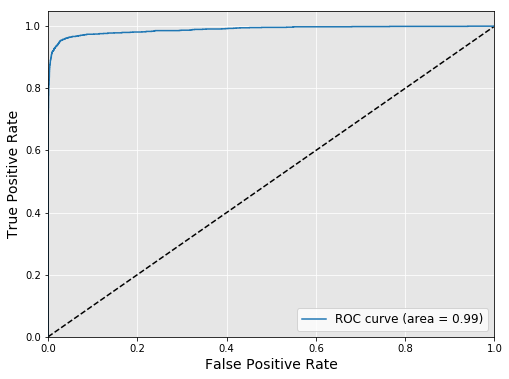
\includegraphics[width=80mm]{imagenes/ROC_Exp2_1.png}} &
				\addheight{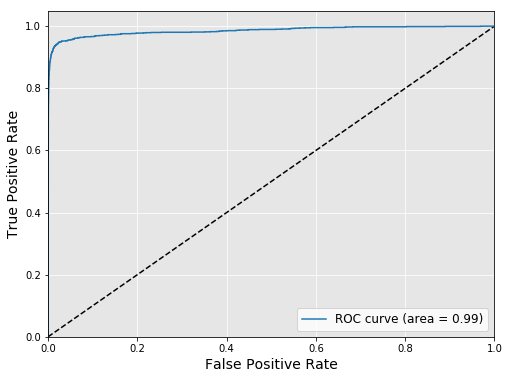
\includegraphics[width=80mm]{imagenes/ROC_Exp2_2.png}}              \\
				\small Segmento 1                                                 & Segmento 2 \\

				\addheight{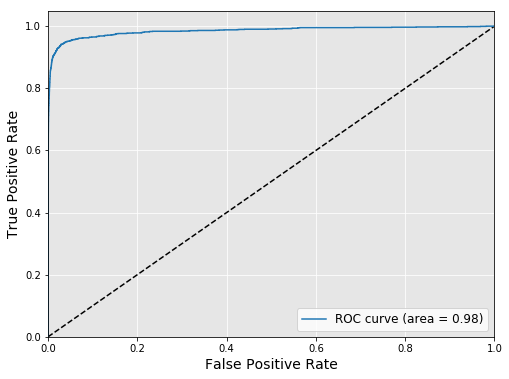
\includegraphics[width=80mm]{imagenes/ROC_Exp2_3.png}} &
				\addheight{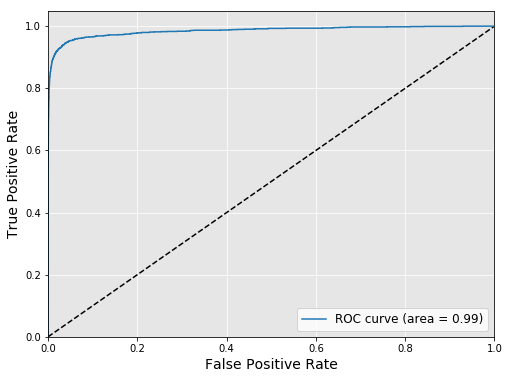
\includegraphics[width=80mm]{imagenes/ROC_Exp2_4.png}}              \\
				\small Segmento 3                                                 & Segmento 4 \\

				\addheight{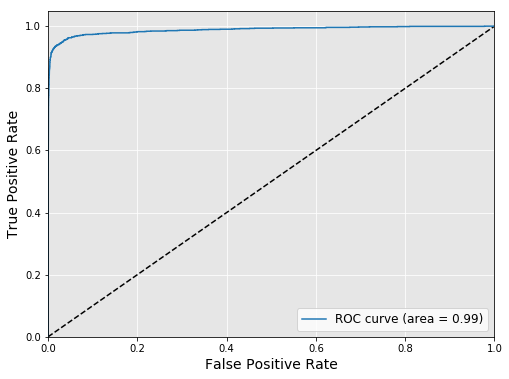
\includegraphics[width=80mm]{imagenes/ROC_Exp2_5.png}} &
				\\
				\small Segmento 5                                                 &            \\
			\end{tabular}
		}

	\end{table}
	\caption{Gráficas ROC de los segmentos en que se dividió el corpus. Segundo experimento por caracteres n-gram  es 1. Se puede notar un crecimiento abrupto al inicio de la gráfica, lo cuál indica que las predicciones se separan más, con respecto al experimento 1. Se puede notar una mejora en el desarrollo de la recta, siendo más suave en la mayoría de las gráficas. Además, hay una mejora significativa en el área bajo la curva, llegando a 0.99.}

	\label{fig:Roc2}
\end{figure}
\par Se puede notar que los segmentos de este experimento están siempre tiene un AUC por encima del máximo del experimento 1. Lo cual indica directamente que es un mejor modelo.

\subsection{Propuesta de mejora} %%Hasta aqui revise 15 Abril

\par Al analizar los resultados obtenidos se pudo observar una mejora considerable, tanto el \textit{recall} como en \textit{precision} lo que indica que este modelo es mucho mejor que el primero. Esto puede ser debido a que en las redes sociales las reglas gramaticales y de ortografía son más flexibles, y para poner un ejemplo: escribir
``hola ¿Que haces?'' es lo mismo que decir ``ola k ase'', semánticamente hablando, por lo que analizando palabra por palabra la similitud entre estas palabras es pequeña mientras que carácter por carácter es más grande debido a la red neuronal puede encontrar secuencias de caracteres que realmente importa como `ola'  y también encontrar una correlación entre `que' y `k' lo cual significaría que se adapta al uso de la lengua.

\par El \textit{recall} como se explicó previamente es la medida que indica qué porcentaje de muestras relevantes es encontrada. Los números indican que en el experimento 1 de 100 muestras irónicas, pudo distinguir 76 y en el experimento 2 pudo distinguir 86. Mientras que el \textit{precision} es la medida que muestra que porcentaje de las muestras clasificadas como irónicas fue de verdad irónica. Por lo tanto en números el experimento 1 detectó 100 muestras irónicas, de las cuales el 90.92 \% fue de verdad irónica y el experimento 2 de 100 detectó 95.52 \% irónicas. En ambas métricas el segundo experimento es mucho mejor.

\par Con el fin de mejorar este resultado se propone aumentar el tamaño del n-gram a dos. Esto aportaría mayor información de la vecindad de los caracteres, pudiendo encontrar mejores patrones que describan más globalmente la esencia de los datos.

\section{Tercer Experimento}
\par En este experimento se incrementó el tamaño de los tokens ahora serán tomados por parejas de caracteres. Por lo que algunos tokens podrían ser los siguientes: `ho', `ol', `la'. Lo que se busca con este experimento es obtener más flexibilidad que cuando procesa por palabra y mayor rigidez que cuando procesa por caracter. Los resultados fueron los siguientes:

\subsection{Evaluación}
\begin{center}
	\begin{table}[h]
    \centering
    \caption{Tabla de métricas experimento 3, análisis por tupla de dos caracteres. Se puede notar una mejora en el valor del reclamo, 0.8958 promedio, lo cual eleva el valor-F a 0.9157 promedio, la desviación estándar se mantiene, aumentando un poco en la precisión y disminuyendo en el reclamo, pero aún así es baja por lo que puede considerarse estable. }
\begin{tabular}{|l|llll|}
\hline
& Exactitud &     Precisión &     Reclamo  &   Valor-F \\ \hline
              
Subdivisión1            &       0.9828  &       0.9311  &       0.8954  &       0.9129  \\ 
Subdivisión2            &       0.9842  &       0.9362  &       0.9031  &       0.9194  \\ 
Subdivisión3            &       0.9824  &       0.9076  &       0.9159  &       0.9117  \\ 
Subdivisión4            &       0.9831  &       0.9436  &       0.8845  &       0.9131  \\ 
Subdivisión5            &       0.9850  &       0.9670  &       0.8798  &       0.9213  \\ \hline
Promedio                &       0.9835  &       0.9371  &       0.8958  &       0.9157  \\ \hline
Desviación estándar     &       0.0010  &       0.0192  &       0.0130  &       0.0039  \\ \hline

% Subdivisión 1 & 0.9793 &   0.9387 &   0.8466 &   0.8903  \\
% Subdivisión 2 & 0.9712 &   0.8597 &   0.8490 &   0.8543  \\
% Subdivisión 3 & 0.9743 &   0.9478 &   0.7912 &   0.8624  \\
% Subdivisión 4 & 0.9686 &   0.9221 &   0.7445 &   0.8239  \\
% Subdivisión 5 & 0.9775 &   0.9199 &   0.8506 &   0.8839  \\ \hline
% Promedio      & 0.9742 &  0.9176 &  0.8164 &  0.8630\\ \hline
\end{tabular}
		     \label{tab:exp3}
\end{table}
\end{center}

\par En la tabla \ref{tab:exp3} se puede ver una mejora leve con respecto al experimento anterior con un promedio de \textit{F-score} de 91.57 \% un aumento de casi 1 \%. A continuación en la figura \ref{fig:Roc3}  se muestran algunas de las gráficas ROC que muestran qué tan bien se desempeña este algoritmo.

\begin{figure}

	\begin{table}[H]
		\centering
		\makebox[10pt][c]{
			\begin{tabular}{cc}

				\addheight{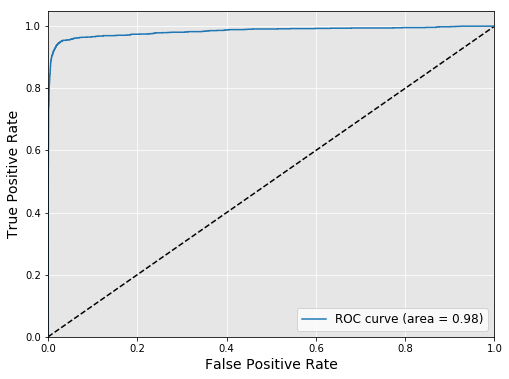
\includegraphics[width=80mm]{imagenes/ROC_Exp3_1.png}} &
				\addheight{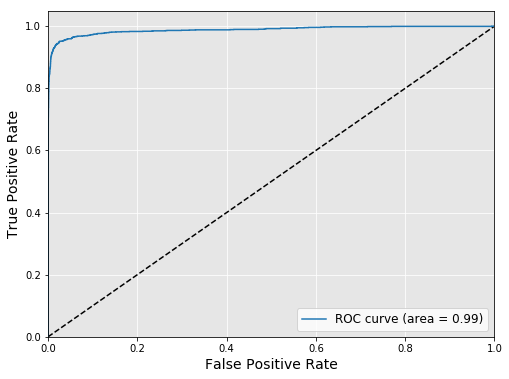
\includegraphics[width=80mm]{imagenes/ROC_Exp3_2.png}}              \\
				\small Segmento 1                                                 & Segmento 2 \\

				\addheight{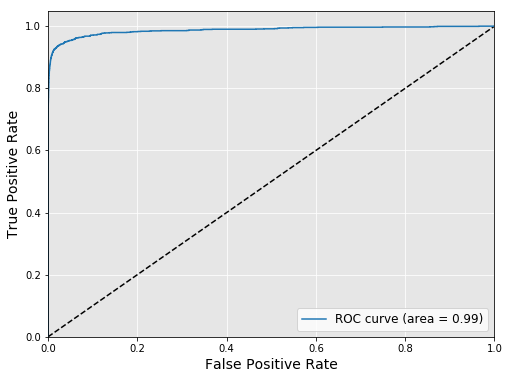
\includegraphics[width=80mm]{imagenes/ROC_Exp3_3.png}} &
				\addheight{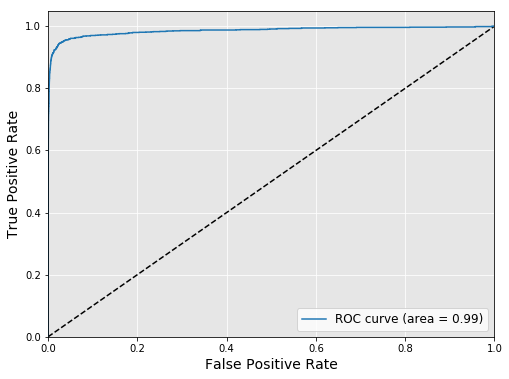
\includegraphics[width=80mm]{imagenes/ROC_Exp3_4.png}}              \\
				\small Segmento 3                                                 & Segmento 4 \\

				\addheight{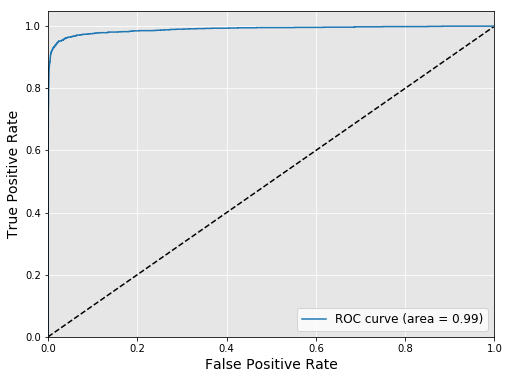
\includegraphics[width=80mm]{imagenes/ROC_Exp3_5.png}} &
				\\
				\small Segmento 5                                                 &            \\
			\end{tabular}
		}

	\end{table}
	\caption{Gráficas ROC de los segmentos en que se dividió el corpus. Tercer experimento por caracteres n-gram  es 2. Se puede notar una mejora sutíl con respecto al segundo experimento. Cabe destacar que el segmento 1 tiene una desarrollo más accidentado, el cuál puede notarse igualmente en experimento dos; esto puede deberse a que la distribución de las muestras es más desfavorable para ese segmento. El área bajo la curva se mantiene en 0.99 y sólo la del segmento 1 es 0.98.}
	\label{fig:Roc3}
\end{figure}



\subsection{Análisis}
\par En este experimento se pudo notar una mejora leve con respecto a los resultados previos. Se pudo ver que los resultados de \textit{accuracy}, \textit{recall} y \textit{f-score} mejoran con respecto al segundo experimento, lo que indica directamente que es un mejor modelo. Sin embargo, la única métrica que no mejora es la \textit{precision} lo que indica que de las muestras que reconoce como irónicas el segundo experimento tiene menores probabilidades de equivocarse. Sin embargo, también tiene menores probabilidades de encontrar las muestras irónicas (\textit{recall}). Y si consideramos el promedio de las dos métricas, se comporta mejor este modelo que el primero.

\par Como propuesta para siguientes experimentos, puede aumentarse el tamaño del n-gram para tratar de encontrar un punto medio que mejore estas métricas, aunque probablemente ya se haya encontrado o esté por encontrarse.

\begin{figure}
	\centering
	
\includegraphics[width=0.7\textwidth]{imagenes/ironia1.png}
	\caption{Texto irónico tomado a prueba. En esta muestra se obtuvo un 0.997028 de porcentaje de ironía. Para el experimento 3.} %%%ACTUALIZAR
	\label{fig:ironyTest1}
\end{figure}

\begin{figure}
	\centering
	
\includegraphics[width=0.7\textwidth]{imagenes/ironia2.png}
	\caption{Texto no irónico tomado a prueba. En esta muestra se obtuvo un 0.0135374 de porcentaje de ironía. Para el experimento 3} %%%ACTUALIZAR
	\label{fig:ironyTest2}
\end{figure}

\par En la figura \ref{fig:ironyTest1} se puede ver que es una muestra irónica que tiene un alto porcentaje de predicción y en la segunda figura \ref{fig:ironyTest2} se puede ver que no es un texto irónico y presenta un bajo porcentaje de predicción. En estas ejemplos se puede ver como se la predicción que hace el sistema.

\section{Cuarto Experimento}

\par En este experimento se probo aumentar el tamaño de la palabra de n-gram, esto con el fin de obtener una mayor flexibilidad que usando como tokens las palabras y una mayor rigidez que cuando se usa n-gram de dos.

\subsection{Evaluación}

\begin{center}
	\begin{table}[h]
	\centering
	\caption{Tabla de métricas experimento 4, por tuplas de 3 caracteres. En esta tabla se puede ver una disminución considerable del F-score, pero un aumente en el recall, además de una disminución en la desviación estándar, lo cual indica que es más estable, en cuando a recall. La precisión cae abruptamente y aumenta considerablemente su desviación estándar.}
\begin{tabular}{|l|llll|}
\hline
& Exactitud &     Precisión &     Recall  &   F-score \\ \hline
              
Subdivisión1            &       0.9754  &       0.8687  &       0.8895  &       0.8790  \\ 
Subdivisión2            &       0.9294  &       0.5959  &       0.9110  &       0.7205  \\ 
Subdivisión3            &       0.8768  &       0.4436  &       0.9409  &       0.6029  \\ 
Subdivisión4            &       0.9364  &       0.6259  &       0.9080  &       0.7410  \\ 
Subdivisión5            &       0.9507  &       0.7014  &       0.8837  &       0.7821  \\ \hline
Promedio                &       0.9338  &       0.6471  &       0.9066  &       0.7451  \\ \hline
Desviación estándar     &       0.0325  &       0.1389  &       0.0200  &       0.0896  \\ \hline



% Subdivisión 1 & 0.9800 & 0.9450 & 0.8479 & 0.8938  \\
% Subdivisión 2 & 0.9787 & 0.9340 & 0.8457 & 0.8877  \\
% Subdivisión 3 & 0.9788 & 0.9414 & 0.8443 & 0.8902  \\
% Subdivisión 4 & 0.9720 & 0.8247 & 0.9093 & 0.8650  \\
% Subdivisión 5 & 0.9743 & 0.8452 & 0.9116 & 0.8771  \\ \hline
% Promedio      & 0.9768 & 0.8718 & 0.8981 & 0.8828  \\ \hline
\end{tabular}
		     \label{tab:exp4}
\end{table}
\end{center}

\par Se puede notar en la tabla \ref{tab:exp4} que el \textit{f-score} es el peor de todos los experimentos, lo cual indica que el equilibrio que se buscaba al aumentar el n-gram ya se había alcanzado con el tercer experimento.

\par Sin embargo, un punto a recalcar en este experimento es que su medida de \textit{recall} es la mejor de los 4 experimentos. Lo cual sería importante si fuera uno de esos problemas en lo que es más importante predecir la mayor parte de las muestras positivas aunque haya muchas veces falsas alarmas, como en sismos, desastres naturales, etc.

\par A continuación en la figura \ref{fig:Roc4}  se muestran algunas de las gráficas ROC que muestran qué tan bien se desempeña este algoritmo. En estas gráficas se puede ver que son peores que la de cualquier experimento, pero siguen teniendo una buena área bajo la curva, lo que indica que es un experimento bastante bueno.

\begin{figure}

	\begin{table}[H]
		\centering
		\makebox[10pt][c]{
			\begin{tabular}{cc}

				\addheight{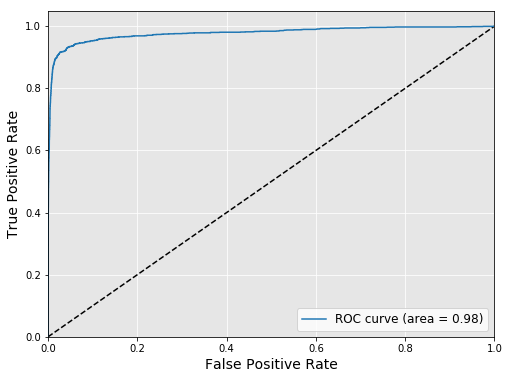
\includegraphics[width=80mm]{imagenes/ROC_Exp4_1.png}} &
				\addheight{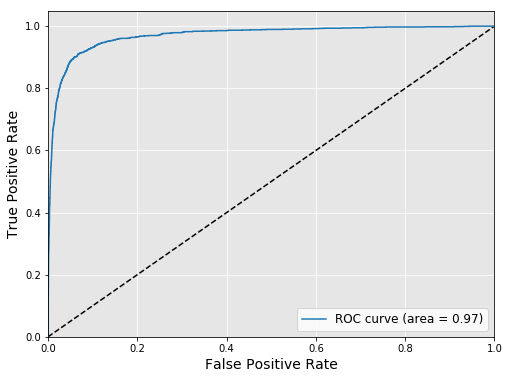
\includegraphics[width=80mm]{imagenes/ROC_Exp4_2.png}}              \\
				\small Segmento 1                                                 & Segmento 2 \\

				\addheight{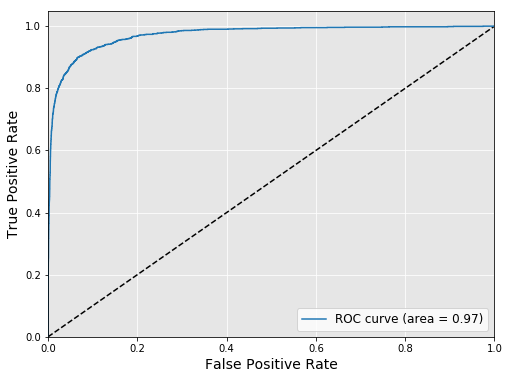
\includegraphics[width=80mm]{imagenes/ROC_Exp4_3.png}} &
				\addheight{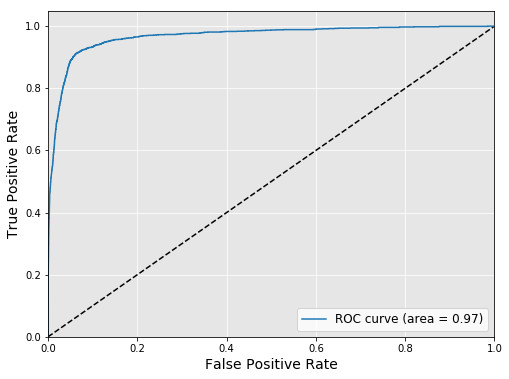
\includegraphics[width=80mm]{imagenes/ROC_Exp4_4.png}}              \\
				\small Segmento 3                                                 & Segmento 4 \\

				\addheight{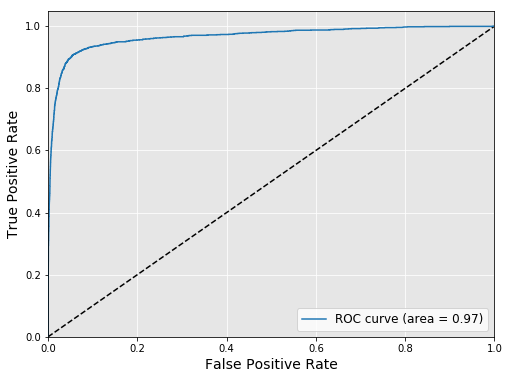
\includegraphics[width=80mm]{imagenes/ROC_Exp4_5.png}} &
				\\
				\small Segmento 5                                                 &            \\
			\end{tabular}
		}

	\end{table}
	\caption{Gráficas ROC de los segmentos en que se dividió el corpus. Cuarto experimento por caracteres n-gram  es 3. Se puede notar una desmejora, general con respecto a los dos experimentos anteriores. Comparado con el experimento 1, este tiene un desarrollo de la recta más suave, lo qué indica que tiene un comportamiento más estable, si se mueve el umbral. El área bajo la curva alcanza a lo más 0.98.}
	\label{fig:Roc4}
\end{figure}

\par En la figura \ref{fig:ironyTest3} y \ref{fig:ironyTest4} se pueden ver ejemplos de cómo el modelo del experimento 4 detecta una muestra irónica y otra que no es irónica.

\begin{figure}[h]
	\centering
	
\includegraphics[width=0.6\textwidth]{imagenes/ironia3.png}
	\caption{Texto medianamente irónico tomado a prueba. En esta muestra se obtuvo un 0.87694 de porcentaje de ironía. Para el experimento 4.} %%%ACTUALIZAR
	\label{fig:ironyTest3}
\end{figure}

\begin{figure}[h]
	\centering
	
\includegraphics[width=0.6\textwidth]{imagenes/ironia4.png}
	\caption{Texto no irónico tomado a prueba. En esta muestra se obtuvo un 0.00296568 de porcentaje de ironía. Para el experimento 4} %%%ACTUALIZAR
	\label{fig:ironyTest4}
\end{figure}

% \begin{figure}[h]
% 	\centering
% 	
\includegraphics[width=0.6\textwidth]{imagenes/ironia1.png}
% 	\caption{Texto irónico tomado a prueba. En esta muestra se obtuvo un 0.998463 de porcentaje de ironía. Para el experimento 4} %%%ACTUALIZAR
% 	\label{fig:ironyTest5}
% \end{figure}
\section{Análisis}
\par Para concluir este capítulo se muestra una tabla que compara directamente las diferentes medidas obtenidas en esta fase de experimentos.

\begin{center}
	\begin{table}[H]
		\centering
		
\begin{tabular}{|l|llll|}
\hline
\# Experimento & Accuracy &     Precision &     Recall  &   F1-score \\ \hline
Experimento 1 (palabras) &       0.9687  &       0.9092  &       0.7669  &       0.8304  \\ \hline
Experimento 2 (1-gram) &       0.9825  &       {\color{OliveGreen} 0.9552}  &       0.8662  &       0.9084  \\ \hline
Experimento 3 (2-gram) &       {\color{OliveGreen} 0.9835}  &       0.9371  &       0.8958  &       {\color{OliveGreen} 0.9157}  \\ \hline
Experimento 4 (3-gram) &       0.9338  &       0.6471  &      {\color{OliveGreen}  0.9066}  &       0.7451  \\ \hline
\end{tabular}
\caption{Tabla total de métricas.}

		\label{tab:total}
	\end{table}
\end{center}

\par En esta tabla se puede notar que el tercer experimento de 2-gram tiene dos métricas mejor que cualquier otro experimento, la primera es el \textit{accuracy} con un 98.35\% y el \textit{F-score} de 91.57\% lo cual está indicando se comporta en general como un mejor modelo que cualquiera de los otros 3. Sin embargo, en el \textit{recall} se puede ver que es mejor el del cuarto experimento, llegando a 90.66\% lo cual como se mencionó puede ser mejor en algunos casos que sea muy importante encontrar la mayor parte de las muestras positivas; sin embargo, su \textit{precision} cae abruptamente. Hablando del \textit{precision} se puede ver que es mejor el segundo experimento, sin dejar caer tanto el \textit{recall} por lo que sería un mejor modelo en un caso en el que se requiera obtener una gran parte de muestras positivas sin disparar tantas falsas alarmas.



\chapter{Conclusiones y trabajo a futuro}\label{cap.conclusiones}

\par Como se mencionó en el capítulo \ref{cap.introduccion} el objetivo era obtener resultados aceptables en la clasificación de la ironía en textos cortos, y por lo visto en el capítulo \ref{cap.experimentos} los resultados descritos se asemejan a los de la bibliografía y en algunos casos superan lo esperado, por lo que el objetivo puede considerarse cumplido. En este proyecto se usa una arquitectura del modelo que ha reportado buen desempeño en la clasificación de reseñas de películas de IMDB. La cual es una tarea que se acerca bastante a la clasificación de la ironía, ya que se trata de extraer una opinión en ambas tareas, la cual puede ser positiva o negativa, en este caso irónica o no irónica.


\begin{table}[H]
	\centering
	
\begin{tabular}{|l|llll|}
\hline
\# Experimento & Accuracy &     Precision &     Recall  &   F1-score \\ \hline
Experimento 1 (palabras) &       0.9687  &       0.9092  &       0.7669  &       0.8304  \\ \hline
Experimento 2 (1-gram) &       0.9825  &       {\color{OliveGreen} 0.9552}  &       0.8662  &       0.9084  \\ \hline
Experimento 3 (2-gram) &       {\color{OliveGreen} 0.9835}  &       0.9371  &       0.8958  &       {\color{OliveGreen} 0.9157}  \\ \hline
Experimento 4 (3-gram) &       0.9338  &       0.6471  &      {\color{OliveGreen}  0.9066}  &       0.7451  \\ \hline
\end{tabular}
\caption{Tabla total de métricas.}

	\label{tab:total2}
\end{table}


\par La tarea de clasificación  de la ironía se ha llevado a cabo por diferentes centros de estudio, con diferentes enfoques y justificaciones, desde los sistemas de reglas que propuso \textcite{utsumi1996unified} a las técnicas modernas como árboles aleatorios \textcite{lopez2016character}. Como se explicó brevemente en el capítulo \ref{cap.experimentos} la tesis presente se enfoca principalmente en definir cual de los 3 enfoques de preprocesamiento se adaptan mejor a la clasificación de la ironía, y resultó que en promedio de \textit{F-score} el mejor modelo fue el del tercer experimento. 

\par A lo largo de los experimentos se pudo ver que sus métricas cambiaban bastante, debido principalmente a como se llevaba a cabo el preprocesamiento. Este preprocesamiento indicó que fue mucho mejor realizar un preprocesamiento por n-gram de dos, debido a que el \textit{F-score} es mejor que en cualquiera de los experimentos. Para retomar un poco el análisis que se realizó en los diferentes experimentos, se describirá brevemente cual fue el preprocesamiento, la configuración de la red neuronal y los resultados.

\par En el primer experimento se tomaron las palabras separadas por signos de puntuación o espacios, como tokens. A estos se les aplicó una discretización, transformándolos a un entero, el cual fue su índice en un diccionario. De este preprocesamiento se extrajeron vectores por tweet, los cuales se pasaron por una red neuronal con una configuración de una capa de embeddings, una de \gls{bi-lstm} y por último una capa totalmente conectada, de la cual se obtenía un 1 si la sentencia fue irónica y un 0 si no lo era. Sus resultados fueron relativamente buenos, ya que obtuvo un promedio de \textit{F-score} de 83.04 \%. Respecto a sus medidas de \textit{precision} y \textit{recall}, este experimento tuvo 90.92 \% y 76.69 \% respectivamente.

\par En el segundo experimento se hizo un preprocesamiento llamado n-gram de 1, por carácter. En este experimento no se excluyeron los caracteres especiales. Se tuvo una configuración similar en la red neuronal, con excepción que la entrada ahora fueron vectores de 200 elementos. Sus resultados fueron significativamente mejores que los del primer experimento ya que sube a 90.84 \% de \textit{F-score}. Tanto el \textit{precision} como el \textit{recall} mejoraron teniendo 95.52 \% y 86.62 \% respectivamente. Este segundo modelo se considera por los resultados mejor que el anterior en todo sentido.

\par En el tercer experimento se aumento el n-gram a 2 y se uso la misma red neuronal que la del segundo experimento. Sus resultados fueron ligeramente mejores que el anterior, llegando a tener un 91.57 \% de \textit{F-score}. Sin embargo, el \textit{precision}
disminuye a 93.71 \%, pero aumenta el \textit{recall} a 89.58 \%. Por estas pequeñas diferencias se podría considerar un mejor modelo el del tercer experimento. No obstante, si se desea un modelo que reporte una menor cantidad de falsos positivos, el primer modelo sería mejor.

\par En el cuarto experimento se aumento el n-gram a 3 y se uso la misma configuración de red neuronal. En cuanto a sus resultados fueron los peores de los 4 experimentos. Cayó el \textit{F-score} a 74.51 \%. Su \textit{precision} cayó a 64.71 \%. Sin embargo, su \textit{recall} aumento respecto a cualquier experimento a 90.66 \% lo cual lo hace el experimento con mejor \textit{recall}. Este modelo es el peor de todos en promedio, sin embargo, si lo que se quiere es un sistema que encuentre la mayor cantidad de muestras positivas este es el mejor de todos, aunque terminará prediciendo también una gran cantidad de falsos positivos.

\par El modelo más confiable respecto a las métricas es el tercero por su  promedio de \textit{F-score}, el cual indica que es el mejor equilibrado y que aunque  no es el que tiene el mejor \textit{recall} o \textit{precision} tiene la mayor confiabilidad de los tres ya que se equivocará menos veces.

\par Cabe recalcar que estas son medidas que describen el comportamiento del modelo. Sin embargo, es posible que en algunos problemas sea mucho más importante tener un mejor \textit{precision} o un mejor \textit{recall}. Esto dependerá del uso que tenga el modelo.

\par Por todas estas razones se puede ver que el objetivo de proponer un modelo de red neuronal que pueda identificar la ironía, se ha cumplido. Debido a lo descrito el capítulo \ref{cap.experimentos} se encuentra que el \textit{F-score} promedio del experimento 3, es el mejor del los cuatro experimentos que se realizaron. A pesar de que los resultados son superiores a los reportados en el capítulo \ref{cap.introduccion}, estos no se puede comparar directamente debido a que los corpus usados en la bibliografía confiaban enteramente en que los usuarios etiquetaban correctamente los textos irónicos; no obstante, esto no es así siempre. Si los cálculos reportan que el porcentaje de muestras irónicas es de alrededor del 10\% se debe tener en cuenta que también este porcentaje de muestras etiquetadas como irónicas, pueden no ser irónicas, y pueden aportar información confusa que impactará directamente en el desempeño, y las métricas después no serán fidedignas ya que no se toma en cuenta que no es la ironía lo que se está detectando, sino cuando los usuarios usarán la etiqueta de \#ironía. Como se puede ver en el ejemplo de la figura \ref{fig:ejemploNoironia}.
\begin{figure}
	\centering
	
\includegraphics[width=0.6\linewidth]{imagenes/ejemploIroniaNoironia.png}
	\caption{Ejemplo de una muestra que no esta bien etiquetada.}
	\label{fig:ejemploNoironia}
\end{figure}

\par Por esta razón no se pueden comparar los resultados extraídos en esta ocasión, ya que no hay trabajo previo con el que se puedan comparar directamente. Aún así el modelo aquí propuesto  tiene un desempeño con un 98.35\% de accuracy, 93.71\% de \textit{precision}, 89.58\% de \textit{recall} y 91.57\% de \textit{F-score}, lo cual significa que el 98.35\% de las ocasiones acertará en la clasificación asignada, el 93.71\% de las muestras detectadas como irónicas son de verdad irónicas y el modelo encontrará el 89.58\% de las muestras irónicas. Dicho desempeño puede considerarse bueno ya que su \textit{F-score} supera el 80\% promedio.

\par Como sugerencia para trabajos posteriores se puede establecer una metodología de exploración entre los diferentes modelos que podrían dar mejores resultados. Como la combinación de la arquitectura CNN y la LSTM. Incluso se podrían explorar los nuevos algoritmos de optimación como el Artifitial Plant Optimization o algoritmos genéticos.

\par Por otro lado se pueden implementar o aumentar el preprocesamiento que se usó en este trabajo, tal vez añadiendo etiquetas POS para que éstas aporten diferentes características a la clasificación. Además de esto mi sugerencia es aumentar el tamaño del corpus para obtener una muestra más significativa de la ironía. También puede considerarse una revisión a fondo de los tweets que componen el corpus con el fin de depurar errores de concepto de ironía.

\par Además podría realizarse un estudio en el que se extraigan más clases de ironía como sarcasmo o sátira. Para obtener esto se deben tener claros los conceptos de ironía, sarcasmo y sátira, por lo que se sugiere antes de hacer un modelo que distinga de estos tres, realizar un modelo que distinga el sarcasmo de lo que no lo es, y otro que distinga la sátira de lo que no lo es. Esto sugiero se lleve a cabo en un corpus con muestras irónicas y sarcásticas/satíricas con el fin de que el modelo también pueda distinguir el sarcasmo/sátira de la ironía.

\par Los textos usados en este trabajo proceden de diferentes países. Sin embargo, el idioma no se comporta de la misma manera en todos los lugares donde se habla. Por lo que otro factor a tomar en cuenta para realizar un mejor modelo que detecte mejor la ironía en español es recabar datos de igual tamaño de todos los países donde se hable este idioma. Entonces se tienen dos opciones: realizar el modelo por cada uno de los países realizar otro modelo que detecte de que país es el texto, un problema bastante complejo, y de este modo redirigir el texto al modelo que detecte la ironía para ese país; la otra opción es crear un modelo que tome todo el corpus de todos los países y se entrene para detectar la ironía. Si se realiza de la primera forma se tendrá una forma más certera de encontrar la ironía ya que se adaptaría el modelo a la forma de hablar en ese país. De la segunda forma se ahorraría el primer modelo que clasifique la nación, y solo se tendría que entrenar un modelo, por lo que se ahorraría tiempo. Sin embargo, dado que se usaría la misma arquitectura para detectar la ironía en diferentes países, el modelo tendería a tener un peor desempeño debido a que se entrenaría para un dialecto universal del español, el cual en la realidad no existe. Esto provocaría que se contradiga algunas veces debido a que las mismas palabras tienen diferentes significados en diferentes países.



\newpage

\nocite{*}
\printbibliography[title=Referencias]
\printglossary[type=\acronymtype,title=Abreviaturas]

\newpage
\printglossary[type=main]
\appendix

%     \chapter{Preprocesamiento por palabra}
% 	\lstinputlisting[language=Python,breaklines,numbers=left,
%     stepnumber=1]{codigos/Preprocesamiento.py}

% 	\chapter{Experimento por palabra}
% 	\lstinputlisting[language=Python,breaklines,numbers=left,
%     stepnumber=1]{codigos/experimento1_porpalabras.py}

%     \chapter{Preprocesamiento por caracter}
% 	\lstinputlisting[language=Python,breaklines,numbers=left,
%     stepnumber=1]{codigos/Preprocesamiento2.py}

% 	\chapter{Experimento por caracter}
% 	\lstinputlisting[language=Python,breaklines,numbers=left,
%     stepnumber=1]{codigos/experimento1_porpalabras.py}


%     \chapter{Modelo.json}
%     \lstinputlisting[language=json,firstnumber=1,breaklines,numbers=left]{codigos/modelo.json}


\end{document}